\documentclass[10pt,aspectratio=169]{beamer}
\usetheme{Singapore}%{Frankfurt} %{Madrid}
%\usecolortheme{seahorse}
%!TeX TXS-program:compile = txs:///pdflatex/[--shell-escape]

\usepackage[english]{babel}
\usepackage[utf8]{inputenc}
%\usefonttheme{professionalfonts} % using non standard fonts for beamer
\usepackage{minted}
\usemintedstyle{emacs}
\usepackage{array}
\usefonttheme{serif}     % Font theme: serif
\usepackage{venturis2}
\usepackage[T1]{fontenc}
\usepackage{amssymb}
\usepackage{times}
\usepackage{color}
\usepackage{xcolor} % helps to change color to fbox
\usepackage{hyperref}


\usepackage{float}
\usepackage{graphicx} % Allows including images
\usepackage{svg}
\usepackage{cite}
\usepackage{lipsum}
\usepackage{multirow}
\usepackage{verbatimbox} % As verbatim but takes arguments, for ex fontsize

%---------------------------------------------------------------------------------------------------------------
\renewcommand\fbox{\fcolorbox{red}{white}}
%---------------------------------------------------------------------------------------------------------------
\usepackage{pst-all}	
\usepackage{auto-pst-pdf}
\ifpdf
  \usepackage{tikz}
\else
    \usepackage{pst-all}	
\fi
\usepackage{pstricks} % For current config of Dia psfigures
\setbeamertemplate{caption}[numbered] % For numbering figures
%---------------------------------------------------------------------------------------------------------------
\usepackage{multimedia} % to add videos
\usepackage{media9}
%--------------------------------------------------------------

\mode<presentation> {
\usecolortheme{whale} % Best one
%\setbeamertemplate{footline} % To remove the footer line in all slides uncomment this line
%\setbeamertemplate{footline}[page number] % To replace the footer line in all slides with a simple slide count uncomment this line
%\setbeamertemplate{navigation symbols}{} % To remove the navigation symbols from the bottom of all slides uncomment this line
}

\setbeamercovered{transparent}
\setbeamertemplate{bibliography item}[text]
\setbeamertemplate{theorems}[numbered]
\setbeamerfont{title}{size=\Large}%\miniscule,command,tiny, scriptsize,footnotesize,small,normalsize,large,Large,LARGE,huge,Huge,HUGE
\setbeamerfont{date}{size=\tiny}%{\fontsize{40}{48} \selectfont Text}

\setbeamertemplate{itemize items}[triangle] % if you want a ball
\setbeamertemplate{itemize subitem}[circle] % if you wnat a circle
\setbeamertemplate{itemize subsubitem}[triangle] % if you want a triangle

\newcommand{\bi}{\begin{itemize}\setlength\itemsep{1em}}
\newcommand{\ei}{\end{itemize}}
\newcommand{\bis}{\begin{itemize}}
\newcommand{\eis}{\end{itemize}}

%===============================================
%  COLORS
%===============================================
\definecolor{teal}{RGB}{0,128,128}
\definecolor{magenta}{RGB}{255, 0, 255}
\definecolor{ligthblue}{RGB}{80, 161, 225}
\definecolor{red}{rgb}{0.8, 0, 0}
\definecolor{green}{rgb}{0.0, 0.4, 0.0}
\definecolor{vert}{RGB}{95,190,0}
%\definecolor{vert}{rgb}{0.13,0.545,0.13}
\definecolor{vert2}{rgb}{0.08,0.4,0.}
\definecolor{cement}{RGB}{140,141,135}
\definecolor{lgreyblue}{RGB}{220,230,240}
\definecolor{dgreyblue}{RGB}{110,115,200}
\definecolor{background}{gray}{0.9}
\definecolor{dpipe}{RGB}{0,128,128}
\definecolor{dnode}{RGB}{255, 0, 255}
\definecolor{lbound}{rgb}{0.882353, 0.825071, 0.686107}
\definecolor{dbound}{rgb}{0.582353, 0.525071, 0.386107}
\definecolor{pollito}{RGB}{255, 170, 0.}
\definecolor{vinotinto}{rgb}{0.403922, 0.047059, 0.274510}
\definecolor{tealgreen}{rgb}{0.000000, 0.317647, 0.317647}
\definecolor{lpipe}{rgb}{0.847059, 0.898039, 0.898039}
\definecolor{lnode}{rgb}{0.882353, 0.803922, 0.882353}

\newcommand{\lblue}[1]{\textcolor{ligthblue}{#1}}
\newcommand{\cmag}[1]{\textcolor{magenta}{#1}}
\newcommand{\cgreen}[1]{\textcolor{vert}{#1}}
\newcommand{\cblue}[1]{\textcolor{blue}{#1}}
\newcommand{\bluebf}[1]{\textcolor{blue}{\bf #1}}
\newcommand{\bluebm}[1]{\textcolor{blue}{\bm #1}}
\newcommand{\dgreen}[1]{\textcolor{vert}{#1}}
%\newcommand{\red}[1]{\textcolor{red}{#1}}
\newcommand{\cred}[1]{\textcolor{red}{{#1}}}
\newcommand{\DISMA}[1]{\textcolor{ligthblue}{\textbf{#1}}}
\newcommand{\DENERG}[1]{\textcolor{vert2}{#1}}
\newcommand{\cpipes}[1]{\textcolor{dpipe}{#1}}
\newcommand{\cnodes}[1]{\textcolor{dnode}{#1}}
\newcommand{\cbound}[1]{\textcolor{pollito}{#1}}

%===============================================
% Fontsize def:  between tiny and scriptsize
%===============================================
\makeatletter
\newcommand\notsotiny{\@setfontsize\notsotiny\@vipt\@viipt}
\makeatother

%===============================================
%	TITLE PAGE
%===============================================
\title[Shimmer update]{SHIMMER - Update} 

%\author[AKS]{Ajit Kumar Sahoo \texorpdfstring{\scriptsize Regd No: 16MCPC03}{}}
\author[KC]{
	 \underline{Karol Cascavita}
}
\institute[DISMA]{DISMA - PoliTO} 
\titlegraphic{
%\includesvg[height=1.25 cm]{img_title/unal.svg} \quad

\includegraphics[scale=0.2]{img_other/polito_logo.png}
%\includegraphics[height=1.25 cm]{img_title/saintvenant.png}  \quad
} 


%===============================================
%  INPUT
%===============================================
\input{Macros}

\includeonly{
Intro,
Code_in_memory,
Code_numerical,
Conclusions,
}
%%%%%%%%%%%%%%%%%%%%%%%%%%%%%%%%%%%%%%%%%%%%%%%%%%%%%%%%%%%%%%%%%%
%        DOCUMENT
%%%%%%%%%%%%%%%%%%%%%%%%%%%%%%%%%%%%%%%%%%%%%%%%%%%%%%%%%%%%%%%%%%
 
\begin{document}

%----------------------------------------------------------------
\begin{frame}
\titlepage 
\end{frame}
%----------------------------------------------------------------
%\begin{frame}{TODO}
%\begin{itemize}
%\item explain how the graph it is used 
%	\begin{itemize}
%	\item Computation of volumes
%	\end{itemize}
%\item Fabio's contribution
%\item Gas law template => flexibility with equation of state
%\end{itemize}

%Check Issues for help
%Ideas: Maybe use a sparse matrix for gas mixture, so it is only save the ones in an efficient way. 
%\end{frame}

%----------------------------------------------------------------

\begin{frame}{SHIMMER project requirements (recall)}
\begin{itemize}
\item General description (Page 122)
	\begin{itemize}
    		\item To expand the capabilities of the existent network models available within the consortium and to prepare them for \cblue{open-source release}. 
    		\item \cblue{Validation} and \cblue{benchmarking} of the models against available data and commercial models
	\end{itemize}
\item Requirements for the open-source "model" \DISMA{task 4.2.4} (Page 157)
	\begin{itemize}		
	     \item \cblue{Multi-component} description of gas 
	     \item High-pressure transmission networks
	     \item Highly meshed distribution networks 
	     \item Non-pipe elements
   	\end{itemize}
\item Schedule (Page 135, Fig 6) 
	\begin{itemize}
    \item WP4.2 runs from 1st year to the middle of the last one. 
	\end{itemize}

\item Deliverable (Page 147)
	\begin{itemize}
    \item  Open-source fluid-dynamic "model" with gas quality tracking with \cblue{handbook} and \cblue{tutorials} (Table 7)
    \item \cred{Due date} MS8 Open-source "model" validated \cred{month 18} (Table 8)
	\end{itemize}
\end{itemize}

\red{Publications needed}

\end{frame}
\begin{frame}{Introduction}

\begin{itemize}
\item Develop an \cred{efficient} \cblue{open-source} library in \cblue{C++} for the numerical modelling of natural gas transport through a long-distance network. 
\item Additional requirements: 
	\begin{itemize}
	\item \cred{Steady} and \cred{unsteady} state simulations
	\item Complex \cred{mixture} of gases: hydrogen blending
	\end{itemize}
\item Previous open-source tools in the literature: 
%\begin{itemize}
%    \item SINCAL
%    \item SAInt 
%    \item MYNTS 
%\end{itemize}
    \begin{itemize}
    	\item \textit{GasNetSim} [1]: Steady-regime. Complex mixture composition of gases. \cmag{Python}.
    	\item \textit{Pandapipes} [2]: Steady and quasi-steady regimes in pipes.  Gas mixture evaluated globally (no-varying nodal gas prop).  \cmag{Python}.
    	\item \textit{MORGEN}: Research software for Model Order Reduction order. \cmag{Matlab}.
    \end{itemize} 
\end{itemize}


\href{https://ieeexplore.ieee.org/document/9769148} {[1]  \scriptsize Y. Lu, T. Pesch and A. Benigni, "GasNetSim: An Open-Source Package for Gas Network Simulation with Complex Gas Mixture Compositions," 2022 Open Source Modelling and Simulation of Energy Systems (OSMSES), Aachen, Germany, 2022.} \\
{[2] \scriptsize Lohmeier D, Cronbach D, Drauz SR, Braun M, Kneiske TM. Pandapipes: An Open-Source Piping Grid Calculation Package for Multi-Energy Grid Simulations. Sustainability. 2020; 12(23):9899}
%where authors argued GasNetSim is the first open-source tool that allows complex mixture composition of gases. 
%This salient advantage can be only exploited for steady regime till now. The second library has less model flexibility and, as the former, is written in python. The latter stands for Model Reduction for Gas and Energy Networks, being an academic tool developed in Matlab based on the Euler equations, but rich ... models.  
\end{frame}
%----------------------------------------------------------------

%----------------------------------------------------------------

\begin{frame}{Contributions and meetings}
\begin{itemize}
    \item Contributions
    \begin{itemize}
        \item Karol: main shimmer++ developer
        \item Matteo: supervision, shimmer++ developer
        \item Fabio: supervision, GERG developer
        \item Luisa and Marco: theory and code assistance
    \end{itemize}
    
\item Meetings
\small
\begin{table}[H]
\begin{tabular}{lll}
\hline
Date & Attendance & Goal \\
\hline
\small
$16/11/2023$ &	$\DISMA{Fabio}, \DISMA{Karol}, \DISMA{Matteo}$	& \\
$23/11/2023$ &	$\DENERG{Luisa}, \DISMA{Karol}, \DENERG{Marco}$ 	& Questions session\\
$27/11/2023$ &	$\DISMA{Fabio}, \DISMA{Karol}, \DISMA{Matteo}$ &	Study of the theory\\
$\cred{28/11/2023}$ &	$\DISMA{Fabio}, \DISMA{Karol}, \DENERG{Luisa}, \DENERG{Marco}, \DISMA{Matteo}$  &	Questions session \\
$07/12/2023$ &	$\DISMA{Karol}, \DISMA{Matteo}$	& Supervision session \\
$22/12/2024$ &	$\DISMA{Fabio}, \DISMA{Karol}, \DISMA{Matteo}$	& Supervision session: first code presentation \\
$27/12/2024$ &	$\DISMA{Fabio}, \DISMA{Karol}$	&  Help session: matlab and c++ interface\\
$03/01/0024$ & $\DISMA{Fabio}, \DISMA{Karol}$ &	Help session: matlab and c++ interface\\
$16/01/2024$ &	$\DISMA{Karol},\DENERG{Luisa}$  & 	Questions session \\
\hline
\end{tabular}
\end{table}
\end{itemize}

\end{frame}

%----------------------------------------------------------------
\begin{frame}{Repository}
\begin{itemize}
    \item Repository in \url{https://github.com/datafl4sh/shimmer}
\begin{itemize}
    \item Matlab code by \DENERG{DENERG} 
    \item C++ library developed by \DISMA{DISMA}
    \item Tracking of the development campaign in devoted Issues
    \item Documentation of thesis, slides and shimmer project docs
\end{itemize}
\begin{figure}
	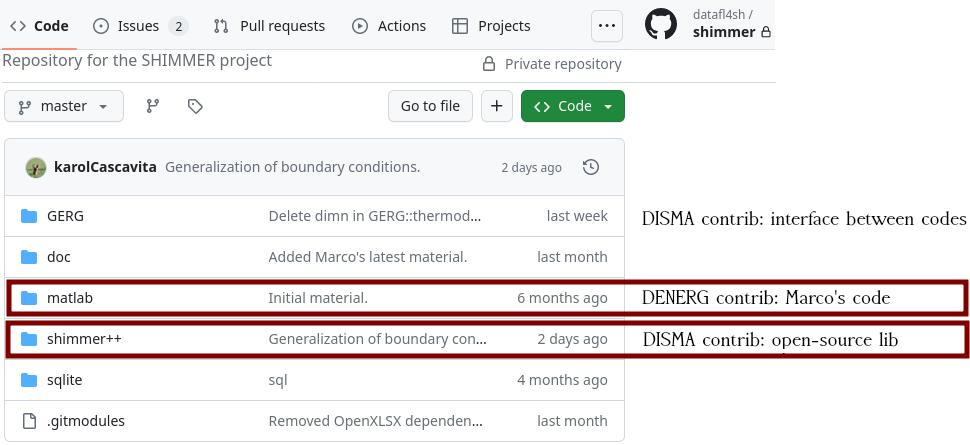
\includegraphics[scale=0.35]{img_other/repo.jpg}
\end{figure}
\item Recommendations:
\begin{itemize}
    \item Do not write in master. Make your branch and make a pull request.
\end{itemize}    
\end{itemize}   
\end{frame}
%----------------------------------------------------------------
\begin{frame}{System boundaries}
\begin{itemize}
    \item Efforts in the in-memory representation and in the numerical methods stages.
\end{itemize}


\begin{figure}[H]
    \centering
    %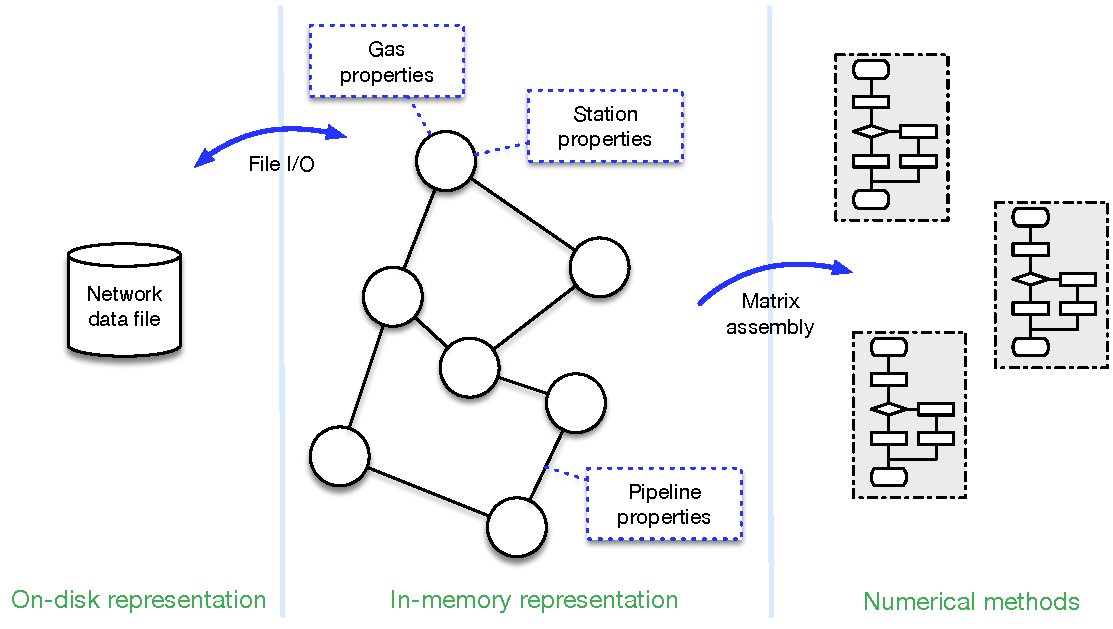
\includegraphics[scale = 0.4]{img_intro/system_arch.pdf}
    \begin{tikzpicture}
    \node[anchor=south west,inner sep=0] (X) at (2, -3) 
    {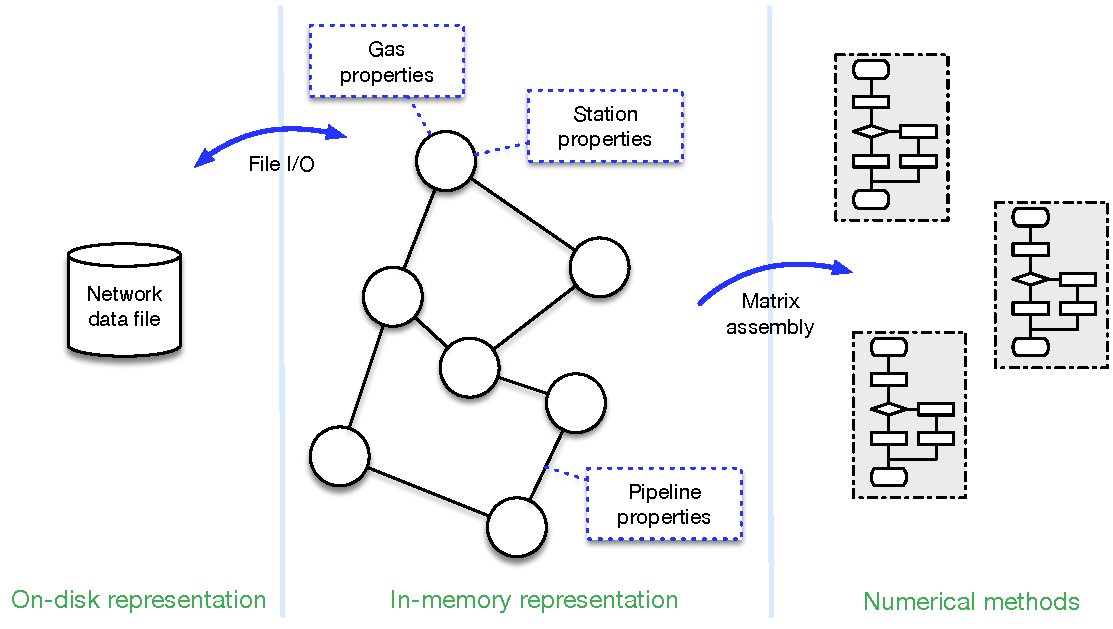
\includegraphics[scale = 0.5]{img_intro/system_arch.pdf}};
    \node [blue, ultra thick] at ($(X.south west)!0.5!(X.north east)$) {};
    % Square for scale 0.4
    %\draw[red] (9.75,-3) -- (9.75,1.25) -- (4.0,1.25) -- (4.0,-3) -- cycle;
    % Square for scale 0.5
    \draw[red] (11.75,-3) -- (11.75,2.25) -- (4.5,2.25) -- (4.5,-3) -- cycle;
    \pgfsetfillcolor{vinotinto}
    \pgfsetfillopacity{0.25}
    \only<2>\fill(8.5,-3) -- (8.5,2.25) -- (4.5,2.25) -- (4.5,-3) -- cycle;   
    \end{tikzpicture}
    \caption{Taken from architecture proposal (Matteo's presentation).}
\end{figure}
   
\end{frame}

%----------------------------------------------------------------
\begin{frame}[fragile]{In-memory representation stage}
\begin{itemize}
\setlength{\itemindent}{-1.0em}
    \item We use a \cred{Boost Graph} Library:  \cblue{generic programming},  \cblue{open-source} and \cblue{header-only} library {
\begin{minted}[linenos=false, frame=single, framesep=2mm,fontsize=\scriptsize]{cpp}
adjacency_list<OutEdgeList, VertexList, Directed, 
               VertexProperties, EdgeProperties, GraphProperties, EdgeList>
\end{minted}      
    }
\item We use an \cred{undirected graph} with values in \cpipes{pipes}/\cnodes{nodes} assigned via the graph properties

% FORKAROL: read for the generic explanation and to open the talk about the given caractheristics of the pipes and nodes by suing boost::graph
% https://www.boost.org/doc/libs/1_82_0/libs/graph/doc/index.html

\begin{center}

\begin{minipage}{0.51\textwidth}
\vspace{-0.25cm}
\begin{minted}[linenos=true,numbersep=1pt,frame=lines,framesep=0.5mm,fontsize=\notsotiny, bgcolor=background]{cpp}
 using namespace boost;
 using graph_type = adjacency_list< listS, vecS,  
                                    undirectedS,
            vertex_properties, edge_properties>;
           
 graph_type graph;
\end{minted}  
\vspace{-0.75cm}
\begin{minted}[linenos=true,numbersep=1pt,frame=lines,framesep=0.5mm,fontsize=\notsotiny]{cpp}
 enum class edge_type {
     pipe,
     resistor,
     compressor,
     regulator,
     valve,
};
 \end{minted}
\vfill
\end{minipage}%
\hfill
\begin{minipage}{0.38\textwidth}
    \begin{minted}[linenos=true,numbersep=1pt,frame=lines,framesep=1.1 mm,fontsize=\notsotiny, bgcolor=background]{cpp}
 struct vertex_properties {
     std::string     name;
     int             number;
     double          height;
     vector_t        gas_mixture;   
 };

 struct edge_properties {
     edge_type   type;
     int         number;
     double      length;
     double      diameter;
     double      friction_factor;
 };  
\end{minted}    
\end{minipage}%    
\end{center}

\item Matrices directly built from graph: Incidence matrix, Resistance matrix, Inertia term
\end{itemize}
\end{frame}

%----------------------------------------------------------------
\begin{frame}[fragile]{Graph initialization}
\begin{itemize}
    \item Graph representation and \cnodes{nodes} specification

    \begin{center}       
    \begin{minipage}{0.25\textwidth}
            \begin{center}
            % Graphic for TeX using PGF
% Title: /home/karol/Documents/UNIVERSITA/POLITO/PRESENTATIONS/SHIMMER_2024_01/img_code/pipe_network.dia
% Creator: Dia v0.97.3
% CreationDate: Mon Jan 22 14:43:56 2024
% For: karol
% \usepackage{tikz}
% The following commands are not supported in PSTricks at present
% We define them conditionally, so when they are implemented,
% this pgf file will use them.
\ifx\du\undefined
  \newlength{\du}
\fi
\setlength{\du}{11\unitlength}
\begin{tikzpicture}[even odd rule]
\pgftransformxscale{1.000000}
\pgftransformyscale{-1.000000}
\definecolor{dialinecolor}{rgb}{0.000000, 0.000000, 0.000000}
\pgfsetstrokecolor{dnode}
\pgfsetstrokeopacity{1.000000}
\definecolor{diafillcolor}{rgb}{1.000000, 1.000000, 1.000000}
\pgfsetfillcolor{diafillcolor}
\pgfsetfillopacity{1.000000}
\pgfsetlinewidth{0.100000\du}
\pgfsetdash{}{0pt}
\pgfsetmiterjoin
\definecolor{diafillcolor}{rgb}{1.000000, 1.000000, 1.000000}
\pgfsetfillcolor{diafillcolor}
\pgfsetfillopacity{1.000000}
\pgfpathellipse{\pgfpoint{8.693572\du}{5.676288\du}}{\pgfpoint{0.693572\du}{0\du}}{\pgfpoint{0\du}{0.676288\du}}
\pgfusepath{fill}
\definecolor{dialinecolor}{rgb}{0.937255, 0.000000, 0.701961}
\pgfsetstrokecolor{dnode}
\pgfsetstrokeopacity{1.000000}
\pgfpathellipse{\pgfpoint{8.693572\du}{5.676288\du}}{\pgfpoint{0.693572\du}{0\du}}{\pgfpoint{0\du}{0.676288\du}}
\pgfusepath{stroke}
% setfont left to latex
% setfont left to latex
\definecolor{dialinecolor}{rgb}{0.000000, 0.000000, 0.000000}
\pgfsetstrokecolor{dnode}
\pgfsetstrokeopacity{1.000000}
\definecolor{diafillcolor}{rgb}{0.000000, 0.000000, 0.000000}
\pgfsetfillcolor{diafillcolor}
\pgfsetfillopacity{1.000000}
\node[anchor=base,inner sep=0pt, outer sep=0pt,color=dnode] at (8.693572\du,5.961288\du){0};
\pgfsetlinewidth{0.100000\du}
\pgfsetdash{}{0pt}
\pgfsetmiterjoin
\definecolor{diafillcolor}{rgb}{1.000000, 1.000000, 1.000000}
\pgfsetfillcolor{diafillcolor}
\pgfsetfillopacity{1.000000}
\pgfpathellipse{\pgfpoint{8.693572\du}{9.676288\du}}{\pgfpoint{0.693572\du}{0\du}}{\pgfpoint{0\du}{0.676288\du}}
\pgfusepath{fill}
\definecolor{dialinecolor}{rgb}{0.937255, 0.000000, 0.701961}
\pgfsetstrokecolor{dnode}
\pgfsetstrokeopacity{1.000000}
\pgfpathellipse{\pgfpoint{8.693572\du}{9.676288\du}}{\pgfpoint{0.693572\du}{0\du}}{\pgfpoint{0\du}{0.676288\du}}
\pgfusepath{stroke}
% setfont left to latex
% setfont left to latex
\definecolor{dialinecolor}{rgb}{0.000000, 0.000000, 0.000000}
\pgfsetstrokecolor{dialinecolor}
\pgfsetstrokeopacity{1.000000}
\definecolor{diafillcolor}{rgb}{0.000000, 0.000000, 0.000000}
\pgfsetfillcolor{diafillcolor}
\pgfsetfillopacity{1.000000}
\node[anchor=base,inner sep=0pt, outer sep=0pt,color=dnode] at (8.693572\du,9.961288\du){1};
\pgfsetlinewidth{0.100000\du}
\pgfsetdash{}{0pt}
\pgfsetmiterjoin
\definecolor{diafillcolor}{rgb}{1.000000, 1.000000, 1.000000}
\pgfsetfillcolor{diafillcolor}
\pgfsetfillopacity{1.000000}
\pgfpathellipse{\pgfpoint{6.753572\du}{13.676288\du}}{\pgfpoint{0.753572\du}{0\du}}{\pgfpoint{0\du}{0.676288\du}}
\pgfusepath{fill}
\definecolor{dialinecolor}{rgb}{0.937255, 0.000000, 0.701961}
\pgfsetstrokecolor{dnode}
\pgfsetstrokeopacity{1.000000}
\pgfpathellipse{\pgfpoint{6.753572\du}{13.676288\du}}{\pgfpoint{0.753572\du}{0\du}}{\pgfpoint{0\du}{0.676288\du}}
\pgfusepath{stroke}
% setfont left to latex
% setfont left to latex
\definecolor{dialinecolor}{rgb}{0.000000, 0.000000, 0.000000}
\pgfsetstrokecolor{dialinecolor}
\pgfsetstrokeopacity{1.000000}
\definecolor{diafillcolor}{rgb}{0.000000, 0.000000, 0.000000}
\pgfsetfillcolor{diafillcolor}
\pgfsetfillopacity{1.000000}
\node[anchor=base,inner sep=0pt, outer sep=0pt,color=dnode] at (6.753572\du,13.961288\du){2};
\pgfsetlinewidth{0.100000\du}
\pgfsetdash{}{0pt}
\pgfsetmiterjoin
\definecolor{diafillcolor}{rgb}{1.000000, 1.000000, 1.000000}
\pgfsetfillcolor{diafillcolor}
\pgfsetfillopacity{1.000000}
\pgfpathellipse{\pgfpoint{14.693572\du}{13.676288\du}}{\pgfpoint{0.693572\du}{0\du}}{\pgfpoint{0\du}{0.676288\du}}
\pgfusepath{fill}
\definecolor{dialinecolor}{rgb}{0.937255, 0.000000, 0.701961}
\pgfsetstrokecolor{dnode}
\pgfsetstrokeopacity{1.000000}
\pgfpathellipse{\pgfpoint{14.693572\du}{13.676288\du}}{\pgfpoint{0.693572\du}{0\du}}{\pgfpoint{0\du}{0.676288\du}}
\pgfusepath{stroke}
% setfont left to latex
% setfont left to latex
\definecolor{dialinecolor}{rgb}{0.000000, 0.000000, 0.000000}
\pgfsetstrokecolor{dialinecolor}
\pgfsetstrokeopacity{1.000000}
\definecolor{diafillcolor}{rgb}{0.000000, 0.000000, 0.000000}
\pgfsetfillcolor{diafillcolor}
\pgfsetfillopacity{1.000000}
\node[anchor=base,inner sep=0pt, outer sep=0pt,color=dnode] at (14.693572\du,13.961288\du){4};
\pgfsetlinewidth{0.100000\du}
\pgfsetdash{}{0pt}
\pgfsetmiterjoin
\definecolor{diafillcolor}{rgb}{1.000000, 1.000000, 1.000000}
\pgfsetfillcolor{diafillcolor}
\pgfsetfillopacity{1.000000}
\pgfpathellipse{\pgfpoint{10.693572\du}{13.676288\du}}{\pgfpoint{0.693572\du}{0\du}}{\pgfpoint{0\du}{0.676288\du}}
\pgfusepath{fill}
\definecolor{dialinecolor}{rgb}{0.937255, 0.000000, 0.701961}
\pgfsetstrokecolor{dnode}
\pgfsetstrokeopacity{1.000000}
\pgfpathellipse{\pgfpoint{10.693572\du}{13.676288\du}}{\pgfpoint{0.693572\du}{0\du}}{\pgfpoint{0\du}{0.676288\du}}
\pgfusepath{stroke}
% setfont left to latex
% setfont left to latex
\definecolor{dialinecolor}{rgb}{0.000000, 0.000000, 0.000000}
\pgfsetstrokecolor{dialinecolor}
\pgfsetstrokeopacity{1.000000}
\definecolor{diafillcolor}{rgb}{0.000000, 0.000000, 0.000000}
\pgfsetfillcolor{diafillcolor}
\pgfsetfillopacity{1.000000}
\node[anchor=base,inner sep=0pt, outer sep=0pt,color=dnode] at (10.693572\du,13.961288\du){3};
\pgfsetlinewidth{0.050000\du}
\pgfsetdash{}{0pt}
\pgfsetbuttcap
{
\definecolor{diafillcolor}{rgb}{0.000000, 0.501961, 0.501961}
\pgfsetfillcolor{diafillcolor}
\pgfsetfillopacity{1.000000}
% was here!!!
\definecolor{dialinecolor}{rgb}{0.000000, 0.501961, 0.501961}
\pgfsetstrokecolor{dpipe}
\pgfsetstrokeopacity{1.000000}
\draw (8.693572\du,6.351417\du)--(8.693570\du,9.000000\du);
}
\pgfsetlinewidth{0.050000\du}
\pgfsetdash{}{0pt}
\pgfsetbuttcap
{
\definecolor{diafillcolor}{rgb}{0.000000, 0.501961, 0.501961}
\pgfsetfillcolor{diafillcolor}
\pgfsetfillopacity{1.000000}
% was here!!!
\definecolor{dialinecolor}{rgb}{0.000000, 0.501961, 0.501961}
\pgfsetstrokecolor{dpipe}
\pgfsetstrokeopacity{1.000000}
\draw (8.693570\du,10.352600\du)--(6.753570\du,13.000000\du);
}
\pgfsetlinewidth{0.050000\du}
\pgfsetdash{}{0pt}
\pgfsetbuttcap
{
\definecolor{diafillcolor}{rgb}{0.000000, 0.501961, 0.501961}
\pgfsetfillcolor{diafillcolor}
\pgfsetfillopacity{1.000000}
% was here!!!
\definecolor{dialinecolor}{rgb}{0.000000, 0.501961, 0.501961}
\pgfsetstrokecolor{dpipe}
\pgfsetstrokeopacity{1.000000}
\draw (8.693570\du,10.352600\du)--(10.693600\du,13.000000\du);
}
\pgfsetlinewidth{0.050000\du}
\pgfsetdash{}{0pt}
\pgfsetbuttcap
{
\definecolor{diafillcolor}{rgb}{0.000000, 0.501961, 0.501961}
\pgfsetfillcolor{diafillcolor}
\pgfsetfillopacity{1.000000}
% was here!!!
\definecolor{dialinecolor}{rgb}{0.000000, 0.501961, 0.501961}
\pgfsetstrokecolor{dpipe}
\pgfsetstrokeopacity{1.000000}
\draw (10.000000\du,13.676300\du)--(7.507140\du,13.676300\du);
}
\pgfsetlinewidth{0.050000\du}
\pgfsetdash{}{0pt}
\pgfsetbuttcap
{
\definecolor{diafillcolor}{rgb}{0.000000, 0.501961, 0.501961}
\pgfsetfillcolor{diafillcolor}
\pgfsetfillopacity{1.000000}
% was here!!!
\definecolor{dialinecolor}{rgb}{0.000000, 0.501961, 0.501961}
\pgfsetstrokecolor{dpipe}
\pgfsetstrokeopacity{1.000000}
\draw (11.387100\du,13.676300\du)--(14.000000\du,13.676300\du);
}
% setfont left to latex
% setfont left to latex
\definecolor{dialinecolor}{rgb}{0.000000, 0.501961, 0.501961}
\pgfsetstrokecolor{dialinecolor}
\pgfsetstrokeopacity{1.000000}
\definecolor{diafillcolor}{rgb}{0.000000, 0.501961, 0.501961}
\pgfsetfillcolor{diafillcolor}
\pgfsetfillopacity{1.000000}
\node[anchor=base west,inner sep=0pt,outer sep=0pt,color=dpipe] at (7.5000000\du,8.000000\du){0};
% setfont left to latex
% setfont left to latex
\definecolor{dialinecolor}{rgb}{0.000000, 0.501961, 0.501961}
\pgfsetstrokecolor{dialinecolor}
\pgfsetstrokeopacity{1.000000}
\definecolor{diafillcolor}{rgb}{0.000000, 0.501961, 0.501961}
\pgfsetfillcolor{diafillcolor}
\pgfsetfillopacity{1.000000}
\node[anchor=base west,inner sep=0pt,outer sep=0pt,color=dpipe] at (6.5000000\du,12.000000\du){3};
% setfont left to latex
% setfont left to latex
\definecolor{dialinecolor}{rgb}{0.000000, 0.501961, 0.501961}
\pgfsetstrokecolor{dialinecolor}
\pgfsetstrokeopacity{1.000000}
\definecolor{diafillcolor}{rgb}{0.000000, 0.501961, 0.501961}
\pgfsetfillcolor{diafillcolor}
\pgfsetfillopacity{1.000000}
\node[anchor=base west,inner sep=0pt,outer sep=0pt,color=dpipe] at (10.5000000\du,12.000000\du){1};
% setfont left to latex
% setfont left to latex
\definecolor{dialinecolor}{rgb}{0.000000, 0.501961, 0.501961}
\pgfsetstrokecolor{dialinecolor}
\pgfsetstrokeopacity{1.000000}
\definecolor{diafillcolor}{rgb}{0.000000, 0.501961, 0.501961}
\pgfsetfillcolor{diafillcolor}
\pgfsetfillopacity{1.000000}
\node[anchor=base west,inner sep=0pt,outer sep=0pt,color=dpipe] at (8.450000\du,14.900000\du){2};
% setfont left to latex
% setfont left to latex
\definecolor{dialinecolor}{rgb}{0.000000, 0.501961, 0.501961}
\pgfsetstrokecolor{dialinecolor}
\pgfsetstrokeopacity{1.000000}
\definecolor{diafillcolor}{rgb}{0.000000, 0.501961, 0.501961}
\pgfsetfillcolor{diafillcolor}
\pgfsetfillopacity{1.000000}
\node[anchor=base west,inner sep=0pt,outer sep=0pt,color=dpipe] at (12.590000\du,14.895000\du){4};
\end{tikzpicture}
    
            \end{center}
    \end{minipage}
    \hfill
    \begin{minipage}{0.65\textwidth}
        \begin{table}
        \footnotesize
        \begin{tabular}{ccrrrcccc}
        &&&&&&&&\\
        \hline 
        &  & \multicolumn{3}{c}{Node properties}  & & \multicolumn{3}{c}{Mixture composition} \\ \cline{3-5} \cline{7-9}     
        \multirow{5}{*}{\rotatebox[origin=c]{90}{\cnodes{Nodes}}} 
        &           & G[kg/s] &p[Pa] &H[m]  && CH4 & N2& \dots \\ \hline
        &\cnodes{0} &	5000  & -60  &10.0  && -& -& -\\
        &\cnodes{1} &	0	  &  20  &20.0  && -& - & -\\
        &\cnodes{2} &	0	  &  25  &30.0  && -& - & -\\ 
        &\cnodes{3} &	0	  &  35  &40.0  && -& - & -\\ 
        &\cnodes{4} &	0	  &  50  &50.0  && -& - & -\\
        \hline
        &&&&&&&&\\
        \end{tabular}
        \end{table}
    \end{minipage}
   \end{center}
\item Insertion of vertices using the $boost::add\_vertex$ function
    \begin{center}
    \begin{minted}[linenos=true,numbersep=1pt,frame=lines,framesep=2mm,fontsize=\scriptsize, bgcolor=background]{cpp}
    // Insert station config (name, no., pressure, flux, height)
    auto v0 = add_vertex( { "Station 0", 0, 5e3,-60, 10}, graph) );
    auto v1 = add_vertex( { "Station 1", 1,  0,  20, 20}, graph) );
    auto v2 = add_vertex( { "Station 2", 2,  0,  25, 30}, graph) );
    auto v3 = add_vertex( { "Station 3", 3,  0,  35, 40}, graph) );
    auto v4 = add_vertex( { "Station 4", 4,  0,  50, 50}, graph) );

    std::vector<vertex_descriptor> vds = {v0,v1,v2,v3,v4};  
    \end{minted}
        
    \end{center}

\end{itemize}

\end{frame}
%----------------------------------------------------------------
\begin{frame}[fragile]{Graph initialization}
\begin{itemize}
    \item Graph representation and \cpipes{pipes} specification   
        \begin{center}
        \begin{minipage}{0.25\textwidth}
            \begin{center}
            % Graphic for TeX using PGF
% Title: /home/karol/Documents/UNIVERSITA/POLITO/PRESENTATIONS/SHIMMER_2024_01/img_code/pipe_network.dia
% Creator: Dia v0.97.3
% CreationDate: Mon Jan 22 14:43:56 2024
% For: karol
% \usepackage{tikz}
% The following commands are not supported in PSTricks at present
% We define them conditionally, so when they are implemented,
% this pgf file will use them.
\ifx\du\undefined
  \newlength{\du}
\fi
\setlength{\du}{11\unitlength}
\begin{tikzpicture}[even odd rule]
\pgftransformxscale{1.000000}
\pgftransformyscale{-1.000000}
\definecolor{dialinecolor}{rgb}{0.000000, 0.000000, 0.000000}
\pgfsetstrokecolor{dnode}
\pgfsetstrokeopacity{1.000000}
\definecolor{diafillcolor}{rgb}{1.000000, 1.000000, 1.000000}
\pgfsetfillcolor{diafillcolor}
\pgfsetfillopacity{1.000000}
\pgfsetlinewidth{0.100000\du}
\pgfsetdash{}{0pt}
\pgfsetmiterjoin
\definecolor{diafillcolor}{rgb}{1.000000, 1.000000, 1.000000}
\pgfsetfillcolor{diafillcolor}
\pgfsetfillopacity{1.000000}
\pgfpathellipse{\pgfpoint{8.693572\du}{5.676288\du}}{\pgfpoint{0.693572\du}{0\du}}{\pgfpoint{0\du}{0.676288\du}}
\pgfusepath{fill}
\definecolor{dialinecolor}{rgb}{0.937255, 0.000000, 0.701961}
\pgfsetstrokecolor{dnode}
\pgfsetstrokeopacity{1.000000}
\pgfpathellipse{\pgfpoint{8.693572\du}{5.676288\du}}{\pgfpoint{0.693572\du}{0\du}}{\pgfpoint{0\du}{0.676288\du}}
\pgfusepath{stroke}
% setfont left to latex
% setfont left to latex
\definecolor{dialinecolor}{rgb}{0.000000, 0.000000, 0.000000}
\pgfsetstrokecolor{dnode}
\pgfsetstrokeopacity{1.000000}
\definecolor{diafillcolor}{rgb}{0.000000, 0.000000, 0.000000}
\pgfsetfillcolor{diafillcolor}
\pgfsetfillopacity{1.000000}
\node[anchor=base,inner sep=0pt, outer sep=0pt,color=dnode] at (8.693572\du,5.961288\du){0};
\pgfsetlinewidth{0.100000\du}
\pgfsetdash{}{0pt}
\pgfsetmiterjoin
\definecolor{diafillcolor}{rgb}{1.000000, 1.000000, 1.000000}
\pgfsetfillcolor{diafillcolor}
\pgfsetfillopacity{1.000000}
\pgfpathellipse{\pgfpoint{8.693572\du}{9.676288\du}}{\pgfpoint{0.693572\du}{0\du}}{\pgfpoint{0\du}{0.676288\du}}
\pgfusepath{fill}
\definecolor{dialinecolor}{rgb}{0.937255, 0.000000, 0.701961}
\pgfsetstrokecolor{dnode}
\pgfsetstrokeopacity{1.000000}
\pgfpathellipse{\pgfpoint{8.693572\du}{9.676288\du}}{\pgfpoint{0.693572\du}{0\du}}{\pgfpoint{0\du}{0.676288\du}}
\pgfusepath{stroke}
% setfont left to latex
% setfont left to latex
\definecolor{dialinecolor}{rgb}{0.000000, 0.000000, 0.000000}
\pgfsetstrokecolor{dialinecolor}
\pgfsetstrokeopacity{1.000000}
\definecolor{diafillcolor}{rgb}{0.000000, 0.000000, 0.000000}
\pgfsetfillcolor{diafillcolor}
\pgfsetfillopacity{1.000000}
\node[anchor=base,inner sep=0pt, outer sep=0pt,color=dnode] at (8.693572\du,9.961288\du){1};
\pgfsetlinewidth{0.100000\du}
\pgfsetdash{}{0pt}
\pgfsetmiterjoin
\definecolor{diafillcolor}{rgb}{1.000000, 1.000000, 1.000000}
\pgfsetfillcolor{diafillcolor}
\pgfsetfillopacity{1.000000}
\pgfpathellipse{\pgfpoint{6.753572\du}{13.676288\du}}{\pgfpoint{0.753572\du}{0\du}}{\pgfpoint{0\du}{0.676288\du}}
\pgfusepath{fill}
\definecolor{dialinecolor}{rgb}{0.937255, 0.000000, 0.701961}
\pgfsetstrokecolor{dnode}
\pgfsetstrokeopacity{1.000000}
\pgfpathellipse{\pgfpoint{6.753572\du}{13.676288\du}}{\pgfpoint{0.753572\du}{0\du}}{\pgfpoint{0\du}{0.676288\du}}
\pgfusepath{stroke}
% setfont left to latex
% setfont left to latex
\definecolor{dialinecolor}{rgb}{0.000000, 0.000000, 0.000000}
\pgfsetstrokecolor{dialinecolor}
\pgfsetstrokeopacity{1.000000}
\definecolor{diafillcolor}{rgb}{0.000000, 0.000000, 0.000000}
\pgfsetfillcolor{diafillcolor}
\pgfsetfillopacity{1.000000}
\node[anchor=base,inner sep=0pt, outer sep=0pt,color=dnode] at (6.753572\du,13.961288\du){2};
\pgfsetlinewidth{0.100000\du}
\pgfsetdash{}{0pt}
\pgfsetmiterjoin
\definecolor{diafillcolor}{rgb}{1.000000, 1.000000, 1.000000}
\pgfsetfillcolor{diafillcolor}
\pgfsetfillopacity{1.000000}
\pgfpathellipse{\pgfpoint{14.693572\du}{13.676288\du}}{\pgfpoint{0.693572\du}{0\du}}{\pgfpoint{0\du}{0.676288\du}}
\pgfusepath{fill}
\definecolor{dialinecolor}{rgb}{0.937255, 0.000000, 0.701961}
\pgfsetstrokecolor{dnode}
\pgfsetstrokeopacity{1.000000}
\pgfpathellipse{\pgfpoint{14.693572\du}{13.676288\du}}{\pgfpoint{0.693572\du}{0\du}}{\pgfpoint{0\du}{0.676288\du}}
\pgfusepath{stroke}
% setfont left to latex
% setfont left to latex
\definecolor{dialinecolor}{rgb}{0.000000, 0.000000, 0.000000}
\pgfsetstrokecolor{dialinecolor}
\pgfsetstrokeopacity{1.000000}
\definecolor{diafillcolor}{rgb}{0.000000, 0.000000, 0.000000}
\pgfsetfillcolor{diafillcolor}
\pgfsetfillopacity{1.000000}
\node[anchor=base,inner sep=0pt, outer sep=0pt,color=dnode] at (14.693572\du,13.961288\du){4};
\pgfsetlinewidth{0.100000\du}
\pgfsetdash{}{0pt}
\pgfsetmiterjoin
\definecolor{diafillcolor}{rgb}{1.000000, 1.000000, 1.000000}
\pgfsetfillcolor{diafillcolor}
\pgfsetfillopacity{1.000000}
\pgfpathellipse{\pgfpoint{10.693572\du}{13.676288\du}}{\pgfpoint{0.693572\du}{0\du}}{\pgfpoint{0\du}{0.676288\du}}
\pgfusepath{fill}
\definecolor{dialinecolor}{rgb}{0.937255, 0.000000, 0.701961}
\pgfsetstrokecolor{dnode}
\pgfsetstrokeopacity{1.000000}
\pgfpathellipse{\pgfpoint{10.693572\du}{13.676288\du}}{\pgfpoint{0.693572\du}{0\du}}{\pgfpoint{0\du}{0.676288\du}}
\pgfusepath{stroke}
% setfont left to latex
% setfont left to latex
\definecolor{dialinecolor}{rgb}{0.000000, 0.000000, 0.000000}
\pgfsetstrokecolor{dialinecolor}
\pgfsetstrokeopacity{1.000000}
\definecolor{diafillcolor}{rgb}{0.000000, 0.000000, 0.000000}
\pgfsetfillcolor{diafillcolor}
\pgfsetfillopacity{1.000000}
\node[anchor=base,inner sep=0pt, outer sep=0pt,color=dnode] at (10.693572\du,13.961288\du){3};
\pgfsetlinewidth{0.050000\du}
\pgfsetdash{}{0pt}
\pgfsetbuttcap
{
\definecolor{diafillcolor}{rgb}{0.000000, 0.501961, 0.501961}
\pgfsetfillcolor{diafillcolor}
\pgfsetfillopacity{1.000000}
% was here!!!
\definecolor{dialinecolor}{rgb}{0.000000, 0.501961, 0.501961}
\pgfsetstrokecolor{dpipe}
\pgfsetstrokeopacity{1.000000}
\draw (8.693572\du,6.351417\du)--(8.693570\du,9.000000\du);
}
\pgfsetlinewidth{0.050000\du}
\pgfsetdash{}{0pt}
\pgfsetbuttcap
{
\definecolor{diafillcolor}{rgb}{0.000000, 0.501961, 0.501961}
\pgfsetfillcolor{diafillcolor}
\pgfsetfillopacity{1.000000}
% was here!!!
\definecolor{dialinecolor}{rgb}{0.000000, 0.501961, 0.501961}
\pgfsetstrokecolor{dpipe}
\pgfsetstrokeopacity{1.000000}
\draw (8.693570\du,10.352600\du)--(6.753570\du,13.000000\du);
}
\pgfsetlinewidth{0.050000\du}
\pgfsetdash{}{0pt}
\pgfsetbuttcap
{
\definecolor{diafillcolor}{rgb}{0.000000, 0.501961, 0.501961}
\pgfsetfillcolor{diafillcolor}
\pgfsetfillopacity{1.000000}
% was here!!!
\definecolor{dialinecolor}{rgb}{0.000000, 0.501961, 0.501961}
\pgfsetstrokecolor{dpipe}
\pgfsetstrokeopacity{1.000000}
\draw (8.693570\du,10.352600\du)--(10.693600\du,13.000000\du);
}
\pgfsetlinewidth{0.050000\du}
\pgfsetdash{}{0pt}
\pgfsetbuttcap
{
\definecolor{diafillcolor}{rgb}{0.000000, 0.501961, 0.501961}
\pgfsetfillcolor{diafillcolor}
\pgfsetfillopacity{1.000000}
% was here!!!
\definecolor{dialinecolor}{rgb}{0.000000, 0.501961, 0.501961}
\pgfsetstrokecolor{dpipe}
\pgfsetstrokeopacity{1.000000}
\draw (10.000000\du,13.676300\du)--(7.507140\du,13.676300\du);
}
\pgfsetlinewidth{0.050000\du}
\pgfsetdash{}{0pt}
\pgfsetbuttcap
{
\definecolor{diafillcolor}{rgb}{0.000000, 0.501961, 0.501961}
\pgfsetfillcolor{diafillcolor}
\pgfsetfillopacity{1.000000}
% was here!!!
\definecolor{dialinecolor}{rgb}{0.000000, 0.501961, 0.501961}
\pgfsetstrokecolor{dpipe}
\pgfsetstrokeopacity{1.000000}
\draw (11.387100\du,13.676300\du)--(14.000000\du,13.676300\du);
}
% setfont left to latex
% setfont left to latex
\definecolor{dialinecolor}{rgb}{0.000000, 0.501961, 0.501961}
\pgfsetstrokecolor{dialinecolor}
\pgfsetstrokeopacity{1.000000}
\definecolor{diafillcolor}{rgb}{0.000000, 0.501961, 0.501961}
\pgfsetfillcolor{diafillcolor}
\pgfsetfillopacity{1.000000}
\node[anchor=base west,inner sep=0pt,outer sep=0pt,color=dpipe] at (7.5000000\du,8.000000\du){0};
% setfont left to latex
% setfont left to latex
\definecolor{dialinecolor}{rgb}{0.000000, 0.501961, 0.501961}
\pgfsetstrokecolor{dialinecolor}
\pgfsetstrokeopacity{1.000000}
\definecolor{diafillcolor}{rgb}{0.000000, 0.501961, 0.501961}
\pgfsetfillcolor{diafillcolor}
\pgfsetfillopacity{1.000000}
\node[anchor=base west,inner sep=0pt,outer sep=0pt,color=dpipe] at (6.5000000\du,12.000000\du){3};
% setfont left to latex
% setfont left to latex
\definecolor{dialinecolor}{rgb}{0.000000, 0.501961, 0.501961}
\pgfsetstrokecolor{dialinecolor}
\pgfsetstrokeopacity{1.000000}
\definecolor{diafillcolor}{rgb}{0.000000, 0.501961, 0.501961}
\pgfsetfillcolor{diafillcolor}
\pgfsetfillopacity{1.000000}
\node[anchor=base west,inner sep=0pt,outer sep=0pt,color=dpipe] at (10.5000000\du,12.000000\du){1};
% setfont left to latex
% setfont left to latex
\definecolor{dialinecolor}{rgb}{0.000000, 0.501961, 0.501961}
\pgfsetstrokecolor{dialinecolor}
\pgfsetstrokeopacity{1.000000}
\definecolor{diafillcolor}{rgb}{0.000000, 0.501961, 0.501961}
\pgfsetfillcolor{diafillcolor}
\pgfsetfillopacity{1.000000}
\node[anchor=base west,inner sep=0pt,outer sep=0pt,color=dpipe] at (8.450000\du,14.900000\du){2};
% setfont left to latex
% setfont left to latex
\definecolor{dialinecolor}{rgb}{0.000000, 0.501961, 0.501961}
\pgfsetstrokecolor{dialinecolor}
\pgfsetstrokeopacity{1.000000}
\definecolor{diafillcolor}{rgb}{0.000000, 0.501961, 0.501961}
\pgfsetfillcolor{diafillcolor}
\pgfsetfillopacity{1.000000}
\node[anchor=base west,inner sep=0pt,outer sep=0pt,color=dpipe] at (12.590000\du,14.895000\du){4};
\end{tikzpicture}
    
            \end{center}
        \end{minipage}
        \hfill
        \begin{minipage}{0.65\textwidth}
            \begin{table}
            \footnotesize
            \begin{tabular}{cccccrrr}
            &&&&&&& \\
            \hline
            &  & \multicolumn{2}{c}{Nodes}&&\multicolumn{3}{c}{Pipe properties} \\ \cline{3-4} \cline{6-8}    
            &  & In	&Out	&&L[m]	&D[m]	&epsi[m] \\ \hline
            \multirow{5}{*}{\rotatebox[origin=c]{90}{\cpipes{Pipes}}}
            &\cpipes{0} &	\cnodes{0} &	\cnodes{1} &&	80.0  &0.6	&1.2e-5 \\
            &\cpipes{1} &	\cnodes{1} &	\cnodes{3} &&	90.0  &0.6	&1.2e-5 \\
            &\cpipes{2} &	\cnodes{3} &	\cnodes{2} &&	100.0 &0.6	&1.2e-5 \\ 
            &\cpipes{3} &	\cnodes{1} &	\cnodes{2} &&	110.0 &0.6	&1.2e-5 \\ 
            &\cpipes{4} &	\cnodes{3} &	\cnodes{4} &&	120.0 &0.6	&1.2e-5 \\ \hline 
            &&&&&&& \\
            \end{tabular}
            \end{table}
        \end{minipage}
        \end{center}
    \item Insertion of pipes using the $boost::add\_edges$ function 
        \begin{center}
        \begin{minted}[linenos=true,numbersep=1pt,frame=lines,framesep=2mm,fontsize=\scriptsize, bgcolor=background]{cpp}
    using pipe_t = edge_type::pipe;

    add_edge( vds[0], vds[1], edge_properties({pipe_t, 0,   80, 0.6, 1.2e-5), graph});
    add_edge( vds[1], vds[3], edge_properties({pipe_t, 1,   90, 0.6, 1.2e-5), graph});
    add_edge( vds[3], vds[2], edge_properties({pipe_t, 2,  100, 0.6, 1.2e-5), graph});
    add_edge( vds[1], vds[2], edge_properties({pipe_t, 3,  110, 0.6, 1.2e-5), graph});
    add_edge( vds[3], vds[4], edge_properties({pipe_t, 4,  120, 0.6, 1.2e-5), graph});
        \end{minted}
        \end{center}
\end{itemize}
\end{frame}
%----------------------------------------------------------------
\begin{frame}[fragile]{Incidence matrix}

\begin{itemize}
    \setlength{\itemindent}{-1.5em}
    \item The incidence matrix establish the connection between nodes and pipes
\end{itemize}

%\hspace{-0.1 cm}
\begin{minipage}{0.35\textwidth}
\begin{minted}[linenos=true,numbersep=1pt,frame=lines,framesep=2mm,fontsize=\notsotiny, bgcolor=background]{cpp}

 class incidence
 {
     sparse_matrix_t mat_;
     sparse_matrix_t mat_in_;
     sparse_matrix_t mat_out_; 
    
     void 
     compute(const graph_type& g);
    
 public:

     incidence(){};
     incidence(const graph_type& g)    
     { 
        compute(g);
     };
    
     const sparse_matrix_t& mat();     
     const sparse_matrix_t& mat_in();   
     const sparse_matrix_t& mat_out();   
 };
 
\end{minted}
\end{minipage}%
\hfill
\hspace{0.2 cm}
\begin{minipage}{0.55\textwidth}

    \begin{minipage}{0.3\textwidth}
         \resizebox{\textwidth}{!}{% Graphic for TeX using PGF
% Title: /home/karol/Documents/UNIVERSITA/POLITO/PRESENTATIONS/SHIMMER_2024_01/img_code/pipe_network.dia
% Creator: Dia v0.97.3
% CreationDate: Mon Jan 22 14:43:56 2024
% For: karol
% \usepackage{tikz}
% The following commands are not supported in PSTricks at present
% We define them conditionally, so when they are implemented,
% this pgf file will use them.
\ifx\du\undefined
  \newlength{\du}
\fi
\setlength{\du}{11\unitlength}
\begin{tikzpicture}[even odd rule]
\pgftransformxscale{1.000000}
\pgftransformyscale{-1.000000}
\definecolor{dialinecolor}{rgb}{0.000000, 0.000000, 0.000000}
\pgfsetstrokecolor{dnode}
\pgfsetstrokeopacity{1.000000}
\definecolor{diafillcolor}{rgb}{1.000000, 1.000000, 1.000000}
\pgfsetfillcolor{diafillcolor}
\pgfsetfillopacity{1.000000}
\pgfsetlinewidth{0.100000\du}
\pgfsetdash{}{0pt}
\pgfsetmiterjoin
\definecolor{diafillcolor}{rgb}{1.000000, 1.000000, 1.000000}
\pgfsetfillcolor{diafillcolor}
\pgfsetfillopacity{1.000000}
\pgfpathellipse{\pgfpoint{8.693572\du}{5.676288\du}}{\pgfpoint{0.693572\du}{0\du}}{\pgfpoint{0\du}{0.676288\du}}
\pgfusepath{fill}
\definecolor{dialinecolor}{rgb}{0.937255, 0.000000, 0.701961}
\pgfsetstrokecolor{dnode}
\pgfsetstrokeopacity{1.000000}
\pgfpathellipse{\pgfpoint{8.693572\du}{5.676288\du}}{\pgfpoint{0.693572\du}{0\du}}{\pgfpoint{0\du}{0.676288\du}}
\pgfusepath{stroke}
% setfont left to latex
% setfont left to latex
\definecolor{dialinecolor}{rgb}{0.000000, 0.000000, 0.000000}
\pgfsetstrokecolor{dnode}
\pgfsetstrokeopacity{1.000000}
\definecolor{diafillcolor}{rgb}{0.000000, 0.000000, 0.000000}
\pgfsetfillcolor{diafillcolor}
\pgfsetfillopacity{1.000000}
\node[anchor=base,inner sep=0pt, outer sep=0pt,color=dnode] at (8.693572\du,5.961288\du){0};
\pgfsetlinewidth{0.100000\du}
\pgfsetdash{}{0pt}
\pgfsetmiterjoin
\definecolor{diafillcolor}{rgb}{1.000000, 1.000000, 1.000000}
\pgfsetfillcolor{diafillcolor}
\pgfsetfillopacity{1.000000}
\pgfpathellipse{\pgfpoint{8.693572\du}{9.676288\du}}{\pgfpoint{0.693572\du}{0\du}}{\pgfpoint{0\du}{0.676288\du}}
\pgfusepath{fill}
\definecolor{dialinecolor}{rgb}{0.937255, 0.000000, 0.701961}
\pgfsetstrokecolor{dnode}
\pgfsetstrokeopacity{1.000000}
\pgfpathellipse{\pgfpoint{8.693572\du}{9.676288\du}}{\pgfpoint{0.693572\du}{0\du}}{\pgfpoint{0\du}{0.676288\du}}
\pgfusepath{stroke}
% setfont left to latex
% setfont left to latex
\definecolor{dialinecolor}{rgb}{0.000000, 0.000000, 0.000000}
\pgfsetstrokecolor{dialinecolor}
\pgfsetstrokeopacity{1.000000}
\definecolor{diafillcolor}{rgb}{0.000000, 0.000000, 0.000000}
\pgfsetfillcolor{diafillcolor}
\pgfsetfillopacity{1.000000}
\node[anchor=base,inner sep=0pt, outer sep=0pt,color=dnode] at (8.693572\du,9.961288\du){1};
\pgfsetlinewidth{0.100000\du}
\pgfsetdash{}{0pt}
\pgfsetmiterjoin
\definecolor{diafillcolor}{rgb}{1.000000, 1.000000, 1.000000}
\pgfsetfillcolor{diafillcolor}
\pgfsetfillopacity{1.000000}
\pgfpathellipse{\pgfpoint{6.753572\du}{13.676288\du}}{\pgfpoint{0.753572\du}{0\du}}{\pgfpoint{0\du}{0.676288\du}}
\pgfusepath{fill}
\definecolor{dialinecolor}{rgb}{0.937255, 0.000000, 0.701961}
\pgfsetstrokecolor{dnode}
\pgfsetstrokeopacity{1.000000}
\pgfpathellipse{\pgfpoint{6.753572\du}{13.676288\du}}{\pgfpoint{0.753572\du}{0\du}}{\pgfpoint{0\du}{0.676288\du}}
\pgfusepath{stroke}
% setfont left to latex
% setfont left to latex
\definecolor{dialinecolor}{rgb}{0.000000, 0.000000, 0.000000}
\pgfsetstrokecolor{dialinecolor}
\pgfsetstrokeopacity{1.000000}
\definecolor{diafillcolor}{rgb}{0.000000, 0.000000, 0.000000}
\pgfsetfillcolor{diafillcolor}
\pgfsetfillopacity{1.000000}
\node[anchor=base,inner sep=0pt, outer sep=0pt,color=dnode] at (6.753572\du,13.961288\du){2};
\pgfsetlinewidth{0.100000\du}
\pgfsetdash{}{0pt}
\pgfsetmiterjoin
\definecolor{diafillcolor}{rgb}{1.000000, 1.000000, 1.000000}
\pgfsetfillcolor{diafillcolor}
\pgfsetfillopacity{1.000000}
\pgfpathellipse{\pgfpoint{14.693572\du}{13.676288\du}}{\pgfpoint{0.693572\du}{0\du}}{\pgfpoint{0\du}{0.676288\du}}
\pgfusepath{fill}
\definecolor{dialinecolor}{rgb}{0.937255, 0.000000, 0.701961}
\pgfsetstrokecolor{dnode}
\pgfsetstrokeopacity{1.000000}
\pgfpathellipse{\pgfpoint{14.693572\du}{13.676288\du}}{\pgfpoint{0.693572\du}{0\du}}{\pgfpoint{0\du}{0.676288\du}}
\pgfusepath{stroke}
% setfont left to latex
% setfont left to latex
\definecolor{dialinecolor}{rgb}{0.000000, 0.000000, 0.000000}
\pgfsetstrokecolor{dialinecolor}
\pgfsetstrokeopacity{1.000000}
\definecolor{diafillcolor}{rgb}{0.000000, 0.000000, 0.000000}
\pgfsetfillcolor{diafillcolor}
\pgfsetfillopacity{1.000000}
\node[anchor=base,inner sep=0pt, outer sep=0pt,color=dnode] at (14.693572\du,13.961288\du){4};
\pgfsetlinewidth{0.100000\du}
\pgfsetdash{}{0pt}
\pgfsetmiterjoin
\definecolor{diafillcolor}{rgb}{1.000000, 1.000000, 1.000000}
\pgfsetfillcolor{diafillcolor}
\pgfsetfillopacity{1.000000}
\pgfpathellipse{\pgfpoint{10.693572\du}{13.676288\du}}{\pgfpoint{0.693572\du}{0\du}}{\pgfpoint{0\du}{0.676288\du}}
\pgfusepath{fill}
\definecolor{dialinecolor}{rgb}{0.937255, 0.000000, 0.701961}
\pgfsetstrokecolor{dnode}
\pgfsetstrokeopacity{1.000000}
\pgfpathellipse{\pgfpoint{10.693572\du}{13.676288\du}}{\pgfpoint{0.693572\du}{0\du}}{\pgfpoint{0\du}{0.676288\du}}
\pgfusepath{stroke}
% setfont left to latex
% setfont left to latex
\definecolor{dialinecolor}{rgb}{0.000000, 0.000000, 0.000000}
\pgfsetstrokecolor{dialinecolor}
\pgfsetstrokeopacity{1.000000}
\definecolor{diafillcolor}{rgb}{0.000000, 0.000000, 0.000000}
\pgfsetfillcolor{diafillcolor}
\pgfsetfillopacity{1.000000}
\node[anchor=base,inner sep=0pt, outer sep=0pt,color=dnode] at (10.693572\du,13.961288\du){3};
\pgfsetlinewidth{0.050000\du}
\pgfsetdash{}{0pt}
\pgfsetbuttcap
{
\definecolor{diafillcolor}{rgb}{0.000000, 0.501961, 0.501961}
\pgfsetfillcolor{diafillcolor}
\pgfsetfillopacity{1.000000}
% was here!!!
\definecolor{dialinecolor}{rgb}{0.000000, 0.501961, 0.501961}
\pgfsetstrokecolor{dpipe}
\pgfsetstrokeopacity{1.000000}
\draw (8.693572\du,6.351417\du)--(8.693570\du,9.000000\du);
}
\pgfsetlinewidth{0.050000\du}
\pgfsetdash{}{0pt}
\pgfsetbuttcap
{
\definecolor{diafillcolor}{rgb}{0.000000, 0.501961, 0.501961}
\pgfsetfillcolor{diafillcolor}
\pgfsetfillopacity{1.000000}
% was here!!!
\definecolor{dialinecolor}{rgb}{0.000000, 0.501961, 0.501961}
\pgfsetstrokecolor{dpipe}
\pgfsetstrokeopacity{1.000000}
\draw (8.693570\du,10.352600\du)--(6.753570\du,13.000000\du);
}
\pgfsetlinewidth{0.050000\du}
\pgfsetdash{}{0pt}
\pgfsetbuttcap
{
\definecolor{diafillcolor}{rgb}{0.000000, 0.501961, 0.501961}
\pgfsetfillcolor{diafillcolor}
\pgfsetfillopacity{1.000000}
% was here!!!
\definecolor{dialinecolor}{rgb}{0.000000, 0.501961, 0.501961}
\pgfsetstrokecolor{dpipe}
\pgfsetstrokeopacity{1.000000}
\draw (8.693570\du,10.352600\du)--(10.693600\du,13.000000\du);
}
\pgfsetlinewidth{0.050000\du}
\pgfsetdash{}{0pt}
\pgfsetbuttcap
{
\definecolor{diafillcolor}{rgb}{0.000000, 0.501961, 0.501961}
\pgfsetfillcolor{diafillcolor}
\pgfsetfillopacity{1.000000}
% was here!!!
\definecolor{dialinecolor}{rgb}{0.000000, 0.501961, 0.501961}
\pgfsetstrokecolor{dpipe}
\pgfsetstrokeopacity{1.000000}
\draw (10.000000\du,13.676300\du)--(7.507140\du,13.676300\du);
}
\pgfsetlinewidth{0.050000\du}
\pgfsetdash{}{0pt}
\pgfsetbuttcap
{
\definecolor{diafillcolor}{rgb}{0.000000, 0.501961, 0.501961}
\pgfsetfillcolor{diafillcolor}
\pgfsetfillopacity{1.000000}
% was here!!!
\definecolor{dialinecolor}{rgb}{0.000000, 0.501961, 0.501961}
\pgfsetstrokecolor{dpipe}
\pgfsetstrokeopacity{1.000000}
\draw (11.387100\du,13.676300\du)--(14.000000\du,13.676300\du);
}
% setfont left to latex
% setfont left to latex
\definecolor{dialinecolor}{rgb}{0.000000, 0.501961, 0.501961}
\pgfsetstrokecolor{dialinecolor}
\pgfsetstrokeopacity{1.000000}
\definecolor{diafillcolor}{rgb}{0.000000, 0.501961, 0.501961}
\pgfsetfillcolor{diafillcolor}
\pgfsetfillopacity{1.000000}
\node[anchor=base west,inner sep=0pt,outer sep=0pt,color=dpipe] at (7.5000000\du,8.000000\du){0};
% setfont left to latex
% setfont left to latex
\definecolor{dialinecolor}{rgb}{0.000000, 0.501961, 0.501961}
\pgfsetstrokecolor{dialinecolor}
\pgfsetstrokeopacity{1.000000}
\definecolor{diafillcolor}{rgb}{0.000000, 0.501961, 0.501961}
\pgfsetfillcolor{diafillcolor}
\pgfsetfillopacity{1.000000}
\node[anchor=base west,inner sep=0pt,outer sep=0pt,color=dpipe] at (6.5000000\du,12.000000\du){3};
% setfont left to latex
% setfont left to latex
\definecolor{dialinecolor}{rgb}{0.000000, 0.501961, 0.501961}
\pgfsetstrokecolor{dialinecolor}
\pgfsetstrokeopacity{1.000000}
\definecolor{diafillcolor}{rgb}{0.000000, 0.501961, 0.501961}
\pgfsetfillcolor{diafillcolor}
\pgfsetfillopacity{1.000000}
\node[anchor=base west,inner sep=0pt,outer sep=0pt,color=dpipe] at (10.5000000\du,12.000000\du){1};
% setfont left to latex
% setfont left to latex
\definecolor{dialinecolor}{rgb}{0.000000, 0.501961, 0.501961}
\pgfsetstrokecolor{dialinecolor}
\pgfsetstrokeopacity{1.000000}
\definecolor{diafillcolor}{rgb}{0.000000, 0.501961, 0.501961}
\pgfsetfillcolor{diafillcolor}
\pgfsetfillopacity{1.000000}
\node[anchor=base west,inner sep=0pt,outer sep=0pt,color=dpipe] at (8.450000\du,14.900000\du){2};
% setfont left to latex
% setfont left to latex
\definecolor{dialinecolor}{rgb}{0.000000, 0.501961, 0.501961}
\pgfsetstrokecolor{dialinecolor}
\pgfsetstrokeopacity{1.000000}
\definecolor{diafillcolor}{rgb}{0.000000, 0.501961, 0.501961}
\pgfsetfillcolor{diafillcolor}
\pgfsetfillopacity{1.000000}
\node[anchor=base west,inner sep=0pt,outer sep=0pt,color=dpipe] at (12.590000\du,14.895000\du){4};
\end{tikzpicture}
 } 
    \end{minipage}%
    \hfill
    \begin{minipage}{0.65\textwidth} 
      \begin{table}
        \scriptsize
        \begin{tabular}{rrrrrrr}
        \hline
        &   & \multicolumn{5}{c}{\cpipes{PIPES}} \\ 
         &  &  \cpipes{0}&  \cpipes{1}&  \cpipes{2}&  \cpipes{3}&  \cpipes{4} \\ \hline
        \multirow{5}{*}{\rotatebox[origin=c]{90}{\cnodes{NODES}}}
         & \cnodes{0}&  1&   &   &   &   \\
         & \cnodes{1}& -1&  1&   &  1&   \\
         & \cnodes{2}&   &   & -1& -1&   \\
         & \cnodes{3}&   & -1&  1&   & 1 \\
         & \cnodes{4}&   &   &   &   &-1 \\ \hline
        \end{tabular}        
        \end{table}
    \end{minipage}    
\begin{minted}[autogobble,escapeinside=||, linenos=true,numbersep=1pt,frame=lines,framesep=2mm,fontsize=\notsotiny, bgcolor=background]{cpp}
   incidence::compute(const graph_type& g)
   { 
      auto range = edges(g);
      for(auto it = range.first;it! = range.second; it++){
          auto pipe = g[*it];   
          auto node_in  = g[source(*it, g)];
          auto node_out = g[target(*it, g)];

          mat_in_( node_in.number,  pipe.number) = 1;
          mat_out_(node_out.number, pipe.number) = 1;       
      }
     mat_ = mat_in_ - mat_out_; 
   }
\end{minted}
\end{minipage}%
 \begin{tikzpicture}[remember picture,overlay]
\only<2>\draw[red] (-3.7,-2.48) -- (-3.7,-2.2) -- (-7.5,-2.2) -- (-7.5,-2.48) -- cycle;
 \end{tikzpicture}
\end{frame}


%----------------------------------------------------------------
\begin{frame}{Numerical methods stage}
\begin{itemize}
    \item Efforts in the in-memory representation and in the numerical methods stages.
\end{itemize}


\begin{figure}[H]
    \centering
    %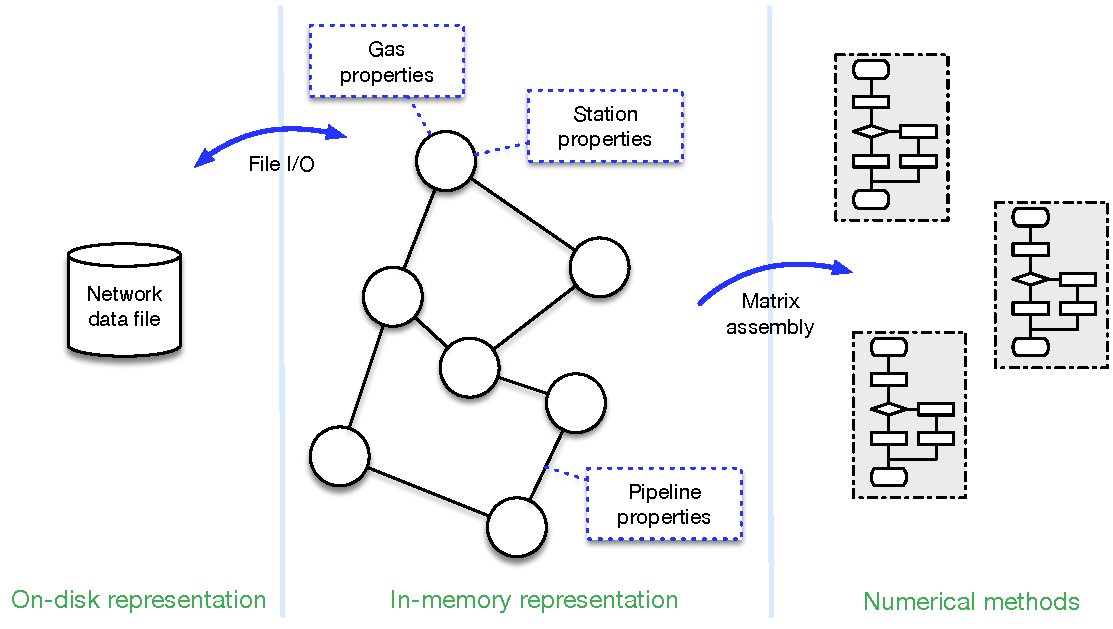
\includegraphics[scale = 0.4]{img_intro/system_arch.pdf}
    \begin{tikzpicture}
    \node[anchor=south west,inner sep=0] (X) at (2, -3) 
    {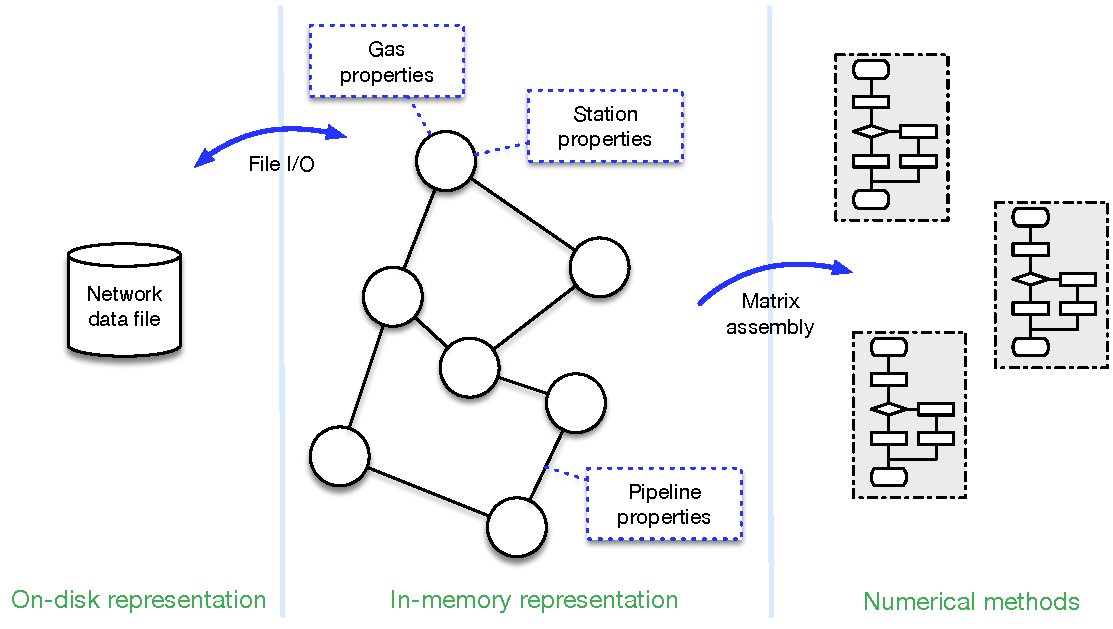
\includegraphics[scale = 0.5]{img_intro/system_arch.pdf}};
    \node [blue, ultra thick] at ($(X.south west)!0.5!(X.north east)$) {};
    % Square for scale 0.4
    %\draw[red] (9.75,-3) -- (9.75,1.25) -- (4.0,1.25) -- (4.0,-3) -- cycle;
    % Square for scale 0.5
    \draw[red] (11.75,-3) -- (11.75,2.25) -- (4.5,2.25) -- (4.5,-3) -- cycle;
    \pgfsetfillcolor{vinotinto}
    \pgfsetfillopacity{0.25}
    \only<2>\fill(8.5,-3) -- (8.5,2.25) -- (4.5,2.25) -- (4.5,-3) -- cycle;
    \only<3>\fill(8.5,-3) -- (8.5,2.25) -- (11.75,2.25) -- (11.75,-3) -- cycle;
    
    \end{tikzpicture}
    \caption{Taken from architecture proposal (Matteo's presentation).}
\end{figure}
   
\end{frame}

%----------------------------------------------------------------
%----------------------------------------------------------------

\begin{frame}{Numerical methods stage}
\noindent
%\psframe[fillstyle=solid,fillcolor=blue!20,linewidth=3pt,linecolor=black](0,0)(21,16)


\begin{minipage}{0.25\textwidth}
% Graphic for TeX using PGF
% Title: /home/karol/Documents/UNIVERSITA/POLITO/PRESENTATIONS/SHIMMER_2024_01/img_code/numerical_methods_algorithm.dia
% Creator: Dia v0.97.3
% CreationDate: Mon Jan 22 14:41:21 2024
% For: karol
% \usepackage{tikz}
% The following commands are not supported in PSTricks at present
% We define them conditionally, so when they are implemented,
% this pgf file will use them.
\ifx\du\undefined
  \newlength{\du}
\fi
\setlength{\du}{7.5\unitlength}
\begin{tikzpicture}[even odd rule]
\pgftransformxscale{1.000000}
\pgftransformyscale{-1.000000}
\definecolor{dialinecolor}{rgb}{0.000000, 0.000000, 0.000000}
\pgfsetstrokecolor{dialinecolor}
\pgfsetstrokeopacity{1.000000}
\definecolor{diafillcolor}{rgb}{1.000000, 1.000000, 1.000000}
\pgfsetfillcolor{diafillcolor}
\pgfsetfillopacity{1.000000}
\pgfsetlinewidth{0.100000\du}
\pgfsetdash{{\pgflinewidth}{0.200000\du}}{0cm}
\pgfsetmiterjoin
\pgfsetbuttcap
{
%\pgfsetcornersarced{\pgfpoint{0.000000\du}{0.000000\du}}\definecolor{diafillcolor}{rgb}{0.898039, 0.898039, 0.898039}
\pgfsetcornersarced{\pgfpoint{0.000000\du}{0.000000\du}}
\pgfsetfillcolor{lgreyblue}
\pgfsetfillopacity{1.000000}
\fill (5.263771\du,-6.474566\du)--(5.263771\du,15.452514\du)--(19.576450\du,15.452514\du)--(19.576450\du,-6.474566\du)--cycle;
}{\pgfsetcornersarced{\pgfpoint{0.000000\du}{0.000000\du}}\definecolor{dialinecolor}{rgb}{0.000000, 0.000000, 0.000000}
% Time stroke
\only<1-2>{\pgfsetstrokecolor{diafillcolor}}
\only<3->{\pgfsetstrokecolor{red}}

\pgfsetstrokeopacity{1.000000}
\draw (5.263771\du,-6.474566\du)--(5.263771\du,15.452514\du)--(19.576450\du,15.452514\du)--(19.576450\du,-6.474566\du)--cycle;
}\pgfsetlinewidth{0.100000\du}
\pgfsetdash{{\pgflinewidth}{0.200000\du}}{0cm}
\pgfsetmiterjoin
\pgfsetbuttcap
{\pgfsetcornersarced{\pgfpoint{0.000000\du}{0.000000\du}}\definecolor{diafillcolor}{rgb}{0.945098, 0.882353, 0.921569}
\pgfsetfillcolor{diafillcolor}
\pgfsetfillopacity{1.000000}
\fill (6.382560\du,-3.393932\du)--(6.382560\du,10.487096\du)--(17.858929\du,10.487096\du)--(17.858929\du,-3.393932\du)--cycle;
}{\pgfsetcornersarced{\pgfpoint{0.000000\du}{0.000000\du}}\definecolor{dialinecolor}{rgb}{0.403922, 0.047059, 0.274510}
\only<1>{\pgfsetstrokecolor{dialinecolor}}
\only<2->{\pgfsetstrokecolor{red}}
\pgfsetstrokeopacity{1.000000}
\draw (6.382560\du,-3.393932\du)--(6.382560\du,10.487096\du)--(17.858929\du,10.487096\du)--(17.858929\du,-3.393932\du)--cycle;
}\pgfsetlinewidth{0.100000\du}
\pgfsetdash{{\pgflinewidth}{0.200000\du}}{0cm}
\pgfsetmiterjoin
\pgfsetbuttcap
{\pgfsetcornersarced{\pgfpoint{0.000000\du}{0.000000\du}}\definecolor{diafillcolor}{rgb}{0.847059, 0.898039, 0.898039}
\pgfsetfillcolor{diafillcolor}
\pgfsetfillopacity{1.000000}
\fill (7.111444\du,-0.032868\du)--(7.111444\du,7.295393\du)--(13.953260\du,7.295393\du)--(13.953260\du,-0.032868\du)--cycle;
}{\pgfsetcornersarced{\pgfpoint{0.000000\du}{0.000000\du}}\definecolor{dialinecolor}{rgb}{0.003876, 0.318700, 0.318700}
\pgfsetstrokecolor{dialinecolor}
\pgfsetstrokeopacity{1.000000}
\draw (7.111444\du,-0.032868\du)--(7.111444\du,7.295393\du)--(13.953260\du,7.295393\du)--(13.953260\du,-0.032868\du)--cycle;
}\pgfsetlinewidth{0.100000\du}
\pgfsetdash{}{0pt}
\pgfsetbuttcap
\pgfsetmiterjoin
\pgfsetlinewidth{0.100000\du}
\pgfsetbuttcap
\pgfsetmiterjoin
\pgfsetdash{}{0pt}
\definecolor{diafillcolor}{rgb}{1.000000, 1.000000, 1.000000}
\pgfsetfillcolor{diafillcolor}
\pgfsetfillopacity{1.000000}
\definecolor{dialinecolor}{rgb}{0.000000, 0.000000, 0.000000}
\pgfsetstrokecolor{dialinecolor}
\pgfsetstrokeopacity{1.000000}
\pgfpathmoveto{\pgfpoint{8.300000\du}{0.200000\du}}
\pgfpathlineto{\pgfpoint{9.900000\du}{0.200000\du}}
\pgfpathcurveto{\pgfpoint{10.120914\du}{0.200000\du}}{\pgfpoint{10.300000\du}{0.401472\du}}{\pgfpoint{10.300000\du}{0.650000\du}}
\pgfpathcurveto{\pgfpoint{10.300000\du}{0.898528\du}}{\pgfpoint{10.120914\du}{1.100000\du}}{\pgfpoint{9.900000\du}{1.100000\du}}
\pgfpathlineto{\pgfpoint{8.300000\du}{1.100000\du}}
\pgfpathcurveto{\pgfpoint{8.079086\du}{1.100000\du}}{\pgfpoint{7.900000\du}{0.898528\du}}{\pgfpoint{7.900000\du}{0.650000\du}}
\pgfpathcurveto{\pgfpoint{7.900000\du}{0.401472\du}}{\pgfpoint{8.079086\du}{0.200000\du}}{\pgfpoint{8.300000\du}{0.200000\du}}
\pgfpathclose
\pgfusepath{fill,stroke}
% setfont left to latex
% setfont left to latex
\definecolor{dialinecolor}{rgb}{0.000000, 0.000000, 0.000000}
\pgfsetstrokecolor{dialinecolor}
\pgfsetstrokeopacity{1.000000}
\definecolor{diafillcolor}{rgb}{0.000000, 0.000000, 0.000000}
\pgfsetfillcolor{diafillcolor}
\pgfsetfillopacity{1.000000}
\node[anchor=base,inner sep=0pt, outer sep=0pt,color=dialinecolor] at (9.100000\du,0.950000\du){};
\pgfsetlinewidth{0.100000\du}
\pgfsetdash{}{0pt}
\pgfsetbuttcap
{
\definecolor{diafillcolor}{rgb}{0.000000, 0.000000, 0.000000}
\pgfsetfillcolor{diafillcolor}
\pgfsetfillopacity{1.000000}
% was here!!!
\definecolor{dialinecolor}{rgb}{0.000000, 0.000000, 0.000000}
\pgfsetstrokecolor{dialinecolor}
\pgfsetstrokeopacity{1.000000}
\draw (9.100000\du,1.100000\du)--(9.100000\du,1.550000\du);
}
\pgfsetlinewidth{0.100000\du}
\pgfsetdash{}{0pt}
\pgfsetmiterjoin
{\pgfsetcornersarced{\pgfpoint{0.000000\du}{0.000000\du}}\definecolor{diafillcolor}{rgb}{1.000000, 1.000000, 1.000000}
\pgfsetfillcolor{diafillcolor}
\pgfsetfillopacity{1.000000}
\fill (7.600000\du,1.550000\du)--(7.600000\du,2.323485\du)--(10.600000\du,2.323485\du)--(10.600000\du,1.550000\du)--cycle;
}{\pgfsetcornersarced{\pgfpoint{0.000000\du}{0.000000\du}}\definecolor{dialinecolor}{rgb}{0.000000, 0.000000, 0.000000}
\pgfsetstrokecolor{dialinecolor}
\pgfsetstrokeopacity{1.000000}
\draw (7.600000\du,1.550000\du)--(7.600000\du,2.323485\du)--(10.600000\du,2.323485\du)--(10.600000\du,1.550000\du)--cycle;
}% setfont left to latex
% setfont left to latex
\definecolor{dialinecolor}{rgb}{0.000000, 0.000000, 0.000000}
\pgfsetstrokecolor{dialinecolor}
\pgfsetstrokeopacity{1.000000}
\definecolor{diafillcolor}{rgb}{0.000000, 0.000000, 0.000000}
\pgfsetfillcolor{diafillcolor}
\pgfsetfillopacity{1.000000}
\node[anchor=base,inner sep=0pt, outer sep=0pt,color=dialinecolor] at (9.100000\du,2.191526\du){};
\pgfsetlinewidth{0.100000\du}
\pgfsetdash{}{0pt}
\pgfsetmiterjoin
\definecolor{diafillcolor}{rgb}{1.000000, 1.000000, 1.000000}
\pgfsetfillcolor{diafillcolor}
\pgfsetfillopacity{1.000000}
\fill (9.099017\du,2.996875\du)--(10.616784\du,3.496875\du)--(9.099017\du,3.996875\du)--(7.581250\du,3.496875\du)--cycle;
\definecolor{dialinecolor}{rgb}{0.000000, 0.000000, 0.000000}
\pgfsetstrokecolor{dialinecolor}
\pgfsetstrokeopacity{1.000000}
\draw (9.099017\du,2.996875\du)--(10.616784\du,3.496875\du)--(9.099017\du,3.996875\du)--(7.581250\du,3.496875\du)--cycle;
% setfont left to latex
% setfont left to latex
\definecolor{dialinecolor}{rgb}{0.000000, 0.000000, 0.000000}
\pgfsetstrokecolor{dialinecolor}
\pgfsetstrokeopacity{1.000000}
\definecolor{diafillcolor}{rgb}{0.000000, 0.000000, 0.000000}
\pgfsetfillcolor{diafillcolor}
\pgfsetfillopacity{1.000000}
\node[anchor=base,inner sep=0pt, outer sep=0pt,color=dialinecolor] at (9.099017\du,3.781875\du){};
\pgfsetlinewidth{0.100000\du}
\pgfsetdash{}{0pt}
\pgfsetbuttcap
{
\definecolor{diafillcolor}{rgb}{0.000000, 0.000000, 0.000000}
\pgfsetfillcolor{diafillcolor}
\pgfsetfillopacity{1.000000}
% was here!!!
\definecolor{dialinecolor}{rgb}{0.000000, 0.000000, 0.000000}
\pgfsetstrokecolor{dialinecolor}
\pgfsetstrokeopacity{1.000000}
\draw (9.099017\du,3.996875\du)--(9.102774\du,4.529549\du);
}
\pgfsetlinewidth{0.100000\du}
\pgfsetdash{}{0pt}
\pgfsetmiterjoin
{\pgfsetcornersarced{\pgfpoint{0.000000\du}{0.000000\du}}\definecolor{diafillcolor}{rgb}{1.000000, 1.000000, 1.000000}
\pgfsetfillcolor{diafillcolor}
\pgfsetfillopacity{1.000000}
\fill (7.602774\du,4.529549\du)--(7.602774\du,5.346335\du)--(10.602774\du,5.346335\du)--(10.602774\du,4.529549\du)--cycle;
}{\pgfsetcornersarced{\pgfpoint{0.000000\du}{0.000000\du}}\definecolor{dialinecolor}{rgb}{0.000000, 0.000000, 0.000000}
\pgfsetstrokecolor{dialinecolor}
\pgfsetstrokeopacity{1.000000}
\draw (7.602774\du,4.529549\du)--(7.602774\du,5.346335\du)--(10.602774\du,5.346335\du)--(10.602774\du,4.529549\du)--cycle;
}% setfont left to latex
% setfont left to latex
\definecolor{dialinecolor}{rgb}{0.000000, 0.000000, 0.000000}
\pgfsetstrokecolor{dialinecolor}
\pgfsetstrokeopacity{1.000000}
\definecolor{diafillcolor}{rgb}{0.000000, 0.000000, 0.000000}
\pgfsetfillcolor{diafillcolor}
\pgfsetfillopacity{1.000000}
\node[anchor=base,inner sep=0pt, outer sep=0pt,color=dialinecolor] at (9.102774\du,5.192725\du){};
\pgfsetlinewidth{0.100000\du}
\pgfsetdash{}{0pt}
\pgfsetbuttcap
{
\definecolor{diafillcolor}{rgb}{0.000000, 0.000000, 0.000000}
\pgfsetfillcolor{diafillcolor}
\pgfsetfillopacity{1.000000}
% was here!!!
\definecolor{dialinecolor}{rgb}{0.000000, 0.000000, 0.000000}
\pgfsetstrokecolor{dialinecolor}
\pgfsetstrokeopacity{1.000000}
\draw (9.100000\du,2.323485\du)--(9.099017\du,2.996875\du);
}
\pgfsetlinewidth{0.100000\du}
\pgfsetdash{}{0pt}
\pgfsetbuttcap
{
\definecolor{diafillcolor}{rgb}{0.000000, 0.000000, 0.000000}
\pgfsetfillcolor{diafillcolor}
\pgfsetfillopacity{1.000000}
% was here!!!
\definecolor{dialinecolor}{rgb}{0.000000, 0.000000, 0.000000}
\pgfsetstrokecolor{dialinecolor}
\pgfsetstrokeopacity{1.000000}
\draw (10.616784\du,3.496875\du)--(11.080431\du,3.494330\du);
}
\pgfsetlinewidth{0.100000\du}
\pgfsetdash{}{0pt}
\pgfsetmiterjoin
{\pgfsetcornersarced{\pgfpoint{0.000000\du}{0.000000\du}}\definecolor{diafillcolor}{rgb}{1.000000, 1.000000, 1.000000}
\pgfsetfillcolor{diafillcolor}
\pgfsetfillopacity{1.000000}
\fill (11.080431\du,3.085936\du)--(11.080431\du,3.902723\du)--(13.643775\du,3.902723\du)--(13.643775\du,3.085936\du)--cycle;
}{\pgfsetcornersarced{\pgfpoint{0.000000\du}{0.000000\du}}\definecolor{dialinecolor}{rgb}{0.000000, 0.000000, 0.000000}
\pgfsetstrokecolor{dialinecolor}
\pgfsetstrokeopacity{1.000000}
\draw (11.080431\du,3.085936\du)--(11.080431\du,3.902723\du)--(13.643775\du,3.902723\du)--(13.643775\du,3.085936\du)--cycle;
}% setfont left to latex
% setfont left to latex
\definecolor{dialinecolor}{rgb}{0.000000, 0.000000, 0.000000}
\pgfsetstrokecolor{dialinecolor}
\pgfsetstrokeopacity{1.000000}
\definecolor{diafillcolor}{rgb}{0.000000, 0.000000, 0.000000}
\pgfsetfillcolor{diafillcolor}
\pgfsetfillopacity{1.000000}
\node[anchor=base,inner sep=0pt, outer sep=0pt,color=dialinecolor] at (12.362103\du,3.749113\du){};
\pgfsetlinewidth{0.100000\du}
\pgfsetdash{}{0pt}
\pgfsetmiterjoin
\pgfsetbuttcap
{
\definecolor{diafillcolor}{rgb}{0.000000, 0.000000, 0.000000}
\pgfsetfillcolor{diafillcolor}
\pgfsetfillopacity{1.000000}
% was here!!!
{\pgfsetcornersarced{\pgfpoint{0.000000\du}{0.000000\du}}\definecolor{dialinecolor}{rgb}{0.000000, 0.000000, 0.000000}
\pgfsetstrokecolor{dialinecolor}
\pgfsetstrokeopacity{1.000000}
\draw (10.602774\du,5.142139\du)--(12.362103\du,5.142139\du)--(12.362103\du,3.902723\du);
}}
\pgfsetlinewidth{0.100000\du}
\pgfsetdash{}{0pt}
\pgfsetbuttcap
\pgfsetmiterjoin
\pgfsetlinewidth{0.100000\du}
\pgfsetbuttcap
\pgfsetmiterjoin
\pgfsetdash{}{0pt}
\definecolor{diafillcolor}{rgb}{1.000000, 1.000000, 1.000000}
\pgfsetfillcolor{diafillcolor}
\pgfsetfillopacity{1.000000}
\definecolor{dialinecolor}{rgb}{0.000000, 0.000000, 0.000000}
\pgfsetstrokecolor{dialinecolor}
\pgfsetstrokeopacity{1.000000}
\pgfpathmoveto{\pgfpoint{8.304290\du}{5.979312\du}}
\pgfpathlineto{\pgfpoint{9.904290\du}{5.979312\du}}
\pgfpathcurveto{\pgfpoint{10.125204\du}{5.979312\du}}{\pgfpoint{10.304290\du}{6.180783\du}}{\pgfpoint{10.304290\du}{6.429312\du}}
\pgfpathcurveto{\pgfpoint{10.304290\du}{6.677840\du}}{\pgfpoint{10.125204\du}{6.879312\du}}{\pgfpoint{9.904290\du}{6.879312\du}}
\pgfpathlineto{\pgfpoint{8.304290\du}{6.879312\du}}
\pgfpathcurveto{\pgfpoint{8.083376\du}{6.879312\du}}{\pgfpoint{7.904290\du}{6.677840\du}}{\pgfpoint{7.904290\du}{6.429312\du}}
\pgfpathcurveto{\pgfpoint{7.904290\du}{6.180783\du}}{\pgfpoint{8.083376\du}{5.979312\du}}{\pgfpoint{8.304290\du}{5.979312\du}}
\pgfpathclose
\pgfusepath{fill,stroke}
% setfont left to latex
% setfont left to latex
\definecolor{dialinecolor}{rgb}{0.000000, 0.000000, 0.000000}
\pgfsetstrokecolor{dialinecolor}
\pgfsetstrokeopacity{1.000000}
\definecolor{diafillcolor}{rgb}{0.000000, 0.000000, 0.000000}
\pgfsetfillcolor{diafillcolor}
\pgfsetfillopacity{1.000000}
\node[anchor=base,inner sep=0pt, outer sep=0pt,color=dialinecolor] at (9.104290\du,6.729312\du){};
\pgfsetlinewidth{0.100000\du}
\pgfsetdash{}{0pt}
\pgfsetbuttcap
{
\definecolor{diafillcolor}{rgb}{0.000000, 0.000000, 0.000000}
\pgfsetfillcolor{diafillcolor}
\pgfsetfillopacity{1.000000}
% was here!!!
\definecolor{dialinecolor}{rgb}{0.000000, 0.000000, 0.000000}
\pgfsetstrokecolor{dialinecolor}
\pgfsetstrokeopacity{1.000000}
\draw (9.102774\du,5.346335\du)--(9.104290\du,5.979312\du);
}
% setfont left to latex
% setfont left to latex
\definecolor{dialinecolor}{rgb}{0.000000, 0.000000, 0.000000}
\pgfsetstrokecolor{dialinecolor}
\pgfsetstrokeopacity{1.000000}
\definecolor{diafillcolor}{rgb}{0.000000, 0.000000, 0.000000}
\pgfsetfillcolor{diafillcolor}
\pgfsetfillopacity{1.000000}
\node[anchor=base west,inner sep=0pt,outer sep=0pt,color=dialinecolor] at (11.506559\du,-0.738088\du){};
% setfont left to latex
% setfont left to latex

\pgfsetstrokecolor{dialinecolor}
\pgfsetstrokeopacity{1.000000}
\pgfsetfillcolor{diafillcolor}
\pgfsetfillopacity{1.000000}
\node[anchor=base west,inner sep=0pt,outer sep=0pt,color=tealgreen] at (11.5\du,0.8 \du){\scriptsize {\textbf{Fluid}}};
\node[anchor=base west,inner sep=0pt,outer sep=0pt,color=tealgreen] at (11.5\du,1.55\du){\scriptsize {\textbf{solver}}};


\definecolor{dialinecolor}{rgb}{0.000000, 0.317647, 0.317647}
\pgfsetstrokecolor{dialinecolor}
\pgfsetstrokeopacity{1.000000}
\definecolor{diafillcolor}{rgb}{0.000000, 0.317647, 0.317647}
\pgfsetfillcolor{red}
\pgfsetfillopacity{1.000000}
% setfont left to latex
% setfont left to latex
\definecolor{dialinecolor}{rgb}{0.000000, 0.317647, 0.317647}
\pgfsetstrokecolor{dialinecolor}
\pgfsetstrokeopacity{1.000000}
\definecolor{diafillcolor}{rgb}{0.000000, 0.317647, 0.317647}
\pgfsetfillcolor{red}
\pgfsetfillopacity{1.000000}
\node[anchor=base west,inner sep=0pt,outer sep=0pt,color=dialinecolor] at (11.178222\du,1.315313\du){};
% setfont left to latex
% setfont left to latex
\definecolor{dialinecolor}{rgb}{0.000000, 0.000000, 0.000000}
\pgfsetstrokecolor{dialinecolor}
\pgfsetstrokeopacity{1.000000}
\definecolor{diafillcolor}{rgb}{0.000000, 0.000000, 0.000000}
\pgfsetfillcolor{diafillcolor}
\pgfsetfillopacity{1.000000}
\node[anchor=base west,inner sep=0pt,outer sep=0pt,color=dialinecolor] at (9.691002\du,-1.143346\du){};
% setfont left to latex
% setfont left to latex
\definecolor{dialinecolor}{rgb}{0.000000, 0.000000, 0.000000}
\pgfsetstrokecolor{dialinecolor}
\pgfsetstrokeopacity{1.000000}
\definecolor{diafillcolor}{rgb}{0.000000, 0.000000, 0.000000}
\pgfsetfillcolor{diafillcolor}
\pgfsetfillopacity{1.000000}
\node[anchor=base west,inner sep=0pt,outer sep=0pt,color=dialinecolor] at (9.766373\du,10.513799\du){};
% setfont left to latex
% setfont left to latex

\pgfsetstrokecolor{red}
\pgfsetstrokeopacity{1.000000}

\only<1>{\node[anchor=base west,inner sep=0pt,outer sep=0pt,color=vinotinto] at (11\du,-1.5\du){\scriptsize \textbf{Quality cycle}}};
\only<2->{\node[anchor=base west,inner sep=0pt,outer sep=0pt,color=red] at (11\du,-1.5\du){\scriptsize \textbf{Quality cycle}};}
\pgfsetlinewidth{0.100000\du}
\pgfsetdash{}{0pt}
\pgfsetbuttcap
{
\definecolor{diafillcolor}{rgb}{0.000000, 0.000000, 0.000000}
\pgfsetfillcolor{diafillcolor}
\pgfsetfillopacity{1.000000}
% was here!!!
\definecolor{dialinecolor}{rgb}{0.000000, 0.000000, 0.000000}
\pgfsetstrokecolor{dialinecolor}
\pgfsetstrokeopacity{1.000000}
\draw (9.099526\du,6.929167\du)--(9.090757\du,7.849149\du);
}
\pgfsetlinewidth{0.100000\du}
\pgfsetdash{}{0pt}
\pgfsetmiterjoin
{\pgfsetcornersarced{\pgfpoint{0.000000\du}{0.000000\du}}\definecolor{diafillcolor}{rgb}{1.000000, 1.000000, 1.000000}
\pgfsetfillcolor{diafillcolor}
\pgfsetfillopacity{1.000000}
\fill (7.590757\du,7.849149\du)--(7.590757\du,8.622634\du)--(10.590757\du,8.622634\du)--(10.590757\du,7.849149\du)--cycle;
}{\pgfsetcornersarced{\pgfpoint{0.000000\du}{0.000000\du}}\definecolor{dialinecolor}{rgb}{0.000000, 0.000000, 0.000000}
\pgfsetstrokecolor{dialinecolor}
\pgfsetstrokeopacity{1.000000}
\draw (7.590757\du,7.849149\du)--(7.590757\du,8.622634\du)--(10.590757\du,8.622634\du)--(10.590757\du,7.849149\du)--cycle;
}% setfont left to latex
% setfont left to latex
\definecolor{dialinecolor}{rgb}{0.000000, 0.000000, 0.000000}
\pgfsetstrokecolor{dialinecolor}
\pgfsetstrokeopacity{1.000000}
\definecolor{diafillcolor}{rgb}{0.000000, 0.000000, 0.000000}
\pgfsetfillcolor{diafillcolor}
\pgfsetfillopacity{1.000000}
\node[anchor=base,inner sep=0pt, outer sep=0pt,color=dialinecolor] at (9.090757\du,8.490675\du){};
\pgfsetlinewidth{0.100000\du}
\pgfsetdash{}{0pt}
\pgfsetmiterjoin
\definecolor{diafillcolor}{rgb}{1.000000, 1.000000, 1.000000}
\pgfsetfillcolor{diafillcolor}
\pgfsetfillopacity{1.000000}
\fill (9.089775\du,8.996139\du)--(10.607542\du,9.496139\du)--(9.089775\du,9.996139\du)--(7.572008\du,9.496139\du)--cycle;
\definecolor{dialinecolor}{rgb}{0.000000, 0.000000, 0.000000}
\pgfsetstrokecolor{dialinecolor}
\pgfsetstrokeopacity{1.000000}
\draw (9.089775\du,8.996139\du)--(10.607542\du,9.496139\du)--(9.089775\du,9.996139\du)--(7.572008\du,9.496139\du)--cycle;
% setfont left to latex
% setfont left to latex
\definecolor{dialinecolor}{rgb}{0.000000, 0.000000, 0.000000}
\pgfsetstrokecolor{dialinecolor}
\pgfsetstrokeopacity{1.000000}
\definecolor{diafillcolor}{rgb}{0.000000, 0.000000, 0.000000}
\pgfsetfillcolor{diafillcolor}
\pgfsetfillopacity{1.000000}
\node[anchor=base,inner sep=0pt, outer sep=0pt,color=dialinecolor] at (9.089775\du,9.781139\du){};
\pgfsetlinewidth{0.100000\du}
\pgfsetdash{}{0pt}
\pgfsetbuttcap
{
\definecolor{diafillcolor}{rgb}{0.000000, 0.000000, 0.000000}
\pgfsetfillcolor{diafillcolor}
\pgfsetfillopacity{1.000000}
% was here!!!
\definecolor{dialinecolor}{rgb}{0.000000, 0.000000, 0.000000}
\pgfsetstrokecolor{dialinecolor}
\pgfsetstrokeopacity{1.000000}
\draw (9.090757\du,8.622634\du)--(9.089775\du,8.996139\du);
}
\pgfsetlinewidth{0.100000\du}
\pgfsetdash{}{0pt}
\pgfsetmiterjoin
{\pgfsetcornersarced{\pgfpoint{0.000000\du}{0.000000\du}}\definecolor{diafillcolor}{rgb}{1.000000, 1.000000, 1.000000}
\pgfsetfillcolor{diafillcolor}
\pgfsetfillopacity{1.000000}
\fill (14.966081\du,7.491214\du)--(14.966081\du,8.308000\du)--(17.529425\du,8.308000\du)--(17.529425\du,7.491214\du)--cycle;
}{\pgfsetcornersarced{\pgfpoint{0.000000\du}{0.000000\du}}\definecolor{dialinecolor}{rgb}{0.000000, 0.000000, 0.000000}
\pgfsetstrokecolor{dialinecolor}
\pgfsetstrokeopacity{1.000000}
\draw (14.966081\du,7.491214\du)--(14.966081\du,8.308000\du)--(17.529425\du,8.308000\du)--(17.529425\du,7.491214\du)--cycle;
}% setfont left to latex
% setfont left to latex
\definecolor{dialinecolor}{rgb}{0.000000, 0.000000, 0.000000}
\pgfsetstrokecolor{dialinecolor}
\pgfsetstrokeopacity{1.000000}
\definecolor{diafillcolor}{rgb}{0.000000, 0.000000, 0.000000}
\pgfsetfillcolor{diafillcolor}
\pgfsetfillopacity{1.000000}
\node[anchor=base,inner sep=0pt, outer sep=0pt,color=dialinecolor] at (16.247753\du,8.154390\du){};
\pgfsetlinewidth{0.100000\du}
\pgfsetdash{}{0pt}
\pgfsetmiterjoin
\pgfsetbuttcap
{
\definecolor{diafillcolor}{rgb}{0.000000, 0.000000, 0.000000}
\pgfsetfillcolor{diafillcolor}
\pgfsetfillopacity{1.000000}
% was here!!!
{\pgfsetcornersarced{\pgfpoint{0.000000\du}{0.000000\du}}\definecolor{dialinecolor}{rgb}{0.000000, 0.000000, 0.000000}
\pgfsetstrokecolor{dialinecolor}
\pgfsetstrokeopacity{1.000000}
\draw (10.607542\du,9.496139\du)--(16.250456\du,9.496139\du)--(16.250456\du,8.308000\du)--(16.247753\du,8.308000\du);
}}
\pgfsetlinewidth{0.100000\du}
\pgfsetdash{}{0pt}
\pgfsetmiterjoin
\pgfsetbuttcap
{
\definecolor{diafillcolor}{rgb}{0.000000, 0.000000, 0.000000}
\pgfsetfillcolor{diafillcolor}
\pgfsetfillopacity{1.000000}
% was here!!!
{\pgfsetcornersarced{\pgfpoint{0.000000\du}{0.000000\du}}\definecolor{dialinecolor}{rgb}{0.000000, 0.000000, 0.000000}
\pgfsetstrokecolor{dialinecolor}
\pgfsetstrokeopacity{1.000000}
\draw (16.247753\du,7.491214\du)--(16.247753\du,-1.240844\du)--(10.609252\du,-1.240844\du)--(10.609252\du,-1.258752\du);
}}
\pgfsetlinewidth{0.100000\du}
\pgfsetdash{}{0pt}
\pgfsetbuttcap
{
\definecolor{diafillcolor}{rgb}{0.000000, 0.000000, 0.000000}
\pgfsetfillcolor{diafillcolor}
\pgfsetfillopacity{1.000000}
% was here!!!
\definecolor{dialinecolor}{rgb}{0.000000, 0.000000, 0.000000}
\pgfsetstrokecolor{dialinecolor}
\pgfsetstrokeopacity{1.000000}
\draw (9.089775\du,9.996139\du)--(9.078930\du,11.105818\du);
}
\pgfsetlinewidth{0.100000\du}
\pgfsetdash{}{0pt}
\pgfsetmiterjoin
{\pgfsetcornersarced{\pgfpoint{0.000000\du}{0.000000\du}}\definecolor{diafillcolor}{rgb}{1.000000, 1.000000, 1.000000}
\pgfsetfillcolor{diafillcolor}
\pgfsetfillopacity{1.000000}
\fill (7.578930\du,11.105818\du)--(7.578930\du,11.879303\du)--(10.578930\du,11.879303\du)--(10.578930\du,11.105818\du)--cycle;
}{\pgfsetcornersarced{\pgfpoint{0.000000\du}{0.000000\du}}\definecolor{dialinecolor}{rgb}{0.000000, 0.000000, 0.000000}
\pgfsetstrokecolor{dialinecolor}
\pgfsetstrokeopacity{1.000000}
\draw (7.578930\du,11.105818\du)--(7.578930\du,11.879303\du)--(10.578930\du,11.879303\du)--(10.578930\du,11.105818\du)--cycle;
}% setfont left to latex
% setfont left to latex
\definecolor{dialinecolor}{rgb}{0.000000, 0.000000, 0.000000}
\pgfsetstrokecolor{dialinecolor}
\pgfsetstrokeopacity{1.000000}
\definecolor{diafillcolor}{rgb}{0.000000, 0.000000, 0.000000}
\pgfsetfillcolor{diafillcolor}
\pgfsetfillopacity{1.000000}
\node[anchor=base,inner sep=0pt, outer sep=0pt,color=dialinecolor] at (9.078930\du,11.747344\du){};
\pgfsetlinewidth{0.100000\du}
\pgfsetdash{}{0pt}
\pgfsetmiterjoin
\definecolor{diafillcolor}{rgb}{1.000000, 1.000000, 1.000000}
\pgfsetfillcolor{diafillcolor}
\pgfsetfillopacity{1.000000}
\fill (9.077947\du,12.443644\du)--(10.595714\du,12.943644\du)--(9.077947\du,13.443644\du)--(7.560180\du,12.943644\du)--cycle;
\definecolor{dialinecolor}{rgb}{0.000000, 0.000000, 0.000000}
\pgfsetstrokecolor{dialinecolor}
\pgfsetstrokeopacity{1.000000}
\draw (9.077947\du,12.443644\du)--(10.595714\du,12.943644\du)--(9.077947\du,13.443644\du)--(7.560180\du,12.943644\du)--cycle;
% setfont left to latex
% setfont left to latex
\definecolor{dialinecolor}{rgb}{0.000000, 0.000000, 0.000000}
\pgfsetstrokecolor{dialinecolor}
\pgfsetstrokeopacity{1.000000}
\definecolor{diafillcolor}{rgb}{0.000000, 0.000000, 0.000000}
\pgfsetfillcolor{diafillcolor}
\pgfsetfillopacity{1.000000}
\node[anchor=base,inner sep=0pt, outer sep=0pt,color=dialinecolor] at (9.077947\du,13.228644\du){};
\pgfsetlinewidth{0.100000\du}
\pgfsetdash{}{0pt}
\pgfsetbuttcap
{
\definecolor{diafillcolor}{rgb}{0.000000, 0.000000, 0.000000}
\pgfsetfillcolor{diafillcolor}
\pgfsetfillopacity{1.000000}
% was here!!!
\definecolor{dialinecolor}{rgb}{0.000000, 0.000000, 0.000000}
\pgfsetstrokecolor{dialinecolor}
\pgfsetstrokeopacity{1.000000}
\draw (9.078930\du,11.879303\du)--(9.077947\du,12.443644\du);
}
\pgfsetlinewidth{0.100000\du}
\pgfsetdash{}{0pt}
\pgfsetmiterjoin
{\pgfsetcornersarced{\pgfpoint{0.000000\du}{0.000000\du}}
\definecolor{diafillcolor}{rgb}{1.000000, 1.000000, 1.000000}
\pgfsetfillcolor{diafillcolor}
\pgfsetfillopacity{1.000000}
\fill (14.790680\du,12.574453\du)--(14.790680\du,13.391240\du)--(17.354023\du,13.391240\du)--(17.354023\du,12.574453\du)--cycle;
}{\pgfsetcornersarced{\pgfpoint{0.000000\du}{0.000000\du}}\definecolor{dialinecolor}{rgb}{0.000000, 0.000000, 0.000000}
\pgfsetstrokecolor{dialinecolor}
\pgfsetstrokeopacity{1.000000}
\draw (14.790680\du,12.574453\du)--(14.790680\du,13.391240\du)--(17.354023\du,13.391240\du)--(17.354023\du,12.574453\du)--cycle;
}% setfont left to latex
% setfont left to latex
\definecolor{dialinecolor}{rgb}{0.000000, 0.000000, 0.000000}
\pgfsetstrokecolor{dialinecolor}
\pgfsetstrokeopacity{1.000000}
\definecolor{diafillcolor}{rgb}{0.000000, 0.000000, 0.000000}
\pgfsetfillcolor{diafillcolor}
\pgfsetfillopacity{1.000000}
\node[anchor=base,inner sep=0pt, outer sep=0pt,color=dialinecolor] at (16.072352\du,13.237630\du){};
\pgfsetlinewidth{0.100000\du}
\pgfsetdash{}{0pt}
\pgfsetmiterjoin
% Quality square
{\pgfsetcornersarced{\pgfpoint{0.000000\du}{0.000000\du}}\definecolor{diafillcolor}{rgb}{1.000000, 1.000000, 1.000000}
\pgfsetfillcolor{diafillcolor}
\pgfsetfillopacity{1.000000}
\fill (7.609252\du,-1.645494\du)--(7.609252\du,-0.872009\du)--(10.609252\du,-0.872009\du)--(10.609252\du,-1.645494\du)--cycle;
}{\pgfsetcornersarced{\pgfpoint{0.000000\du}{0.000000\du}}\definecolor{dialinecolor}{rgb}{0.000000, 0.000000, 0.000000}
\pgfsetstrokecolor{dialinecolor}
\pgfsetstrokeopacity{1.000000}
\draw (7.609252\du,-1.645494\du)--(7.609252\du,-0.872009\du)--(10.609252\du,-0.872009\du)--(10.609252\du,-1.645494\du)--cycle;
}% setfont left to latex
% setfont left to latex
\definecolor{dialinecolor}{rgb}{0.000000, 0.000000, 0.000000}
\pgfsetstrokecolor{dialinecolor}
\pgfsetstrokeopacity{1.000000}
\definecolor{diafillcolor}{rgb}{0.000000, 0.000000, 0.000000}
\pgfsetfillcolor{diafillcolor}
\pgfsetfillopacity{1.000000}
\node[anchor=base,inner sep=0pt, outer sep=0pt,color=dialinecolor] at (9.109252\du,-1.003968\du){};
\pgfsetlinewidth{0.100000\du}
\pgfsetdash{}{0pt}
\pgfsetbuttcap
{
\definecolor{diafillcolor}{rgb}{0.000000, 0.000000, 0.000000}
\pgfsetfillcolor{diafillcolor}
\pgfsetfillopacity{1.000000}
% was here!!!
\definecolor{dialinecolor}{rgb}{0.000000, 0.000000, 0.000000}
\pgfsetstrokecolor{dialinecolor}
\pgfsetstrokeopacity{1.000000}
\draw (10.595714\du,12.943644\du)--(14.790680\du,12.982847\du);
}
\pgfsetlinewidth{0.100000\du}
\pgfsetdash{}{0pt}
\pgfsetmiterjoin
\pgfsetbuttcap
{
\definecolor{diafillcolor}{rgb}{0.000000, 0.000000, 0.000000}
\pgfsetfillcolor{diafillcolor}
\pgfsetfillopacity{1.000000}
% was here!!!
{\pgfsetcornersarced{\pgfpoint{0.000000\du}{0.000000\du}}\definecolor{dialinecolor}{rgb}{0.000000, 0.000000, 0.000000}
\pgfsetstrokecolor{dialinecolor}
\pgfsetstrokeopacity{1.000000}
\draw (17.354023\du,12.982847\du)--(18.785845\du,12.982847\du)--(18.785845\du,-4.157275\du)--(10.600000\du,-4.157275\du)--(10.600000\du,-4.213258\du);
}}
\pgfsetlinewidth{0.100000\du}
\pgfsetdash{}{0pt}
\pgfsetbuttcap
\pgfsetmiterjoin
\pgfsetlinewidth{0.100000\du}
\pgfsetbuttcap
\pgfsetmiterjoin
\pgfsetdash{}{0pt}
\definecolor{diafillcolor}{rgb}{1.000000, 1.000000, 1.000000}
\pgfsetfillcolor{diafillcolor}
\pgfsetfillopacity{1.000000}
\definecolor{dialinecolor}{rgb}{0.000000, 0.000000, 0.000000}
\pgfsetstrokecolor{dialinecolor}
\pgfsetstrokeopacity{1.000000}
\pgfpathmoveto{\pgfpoint{8.304612\du}{-3.013131\du}}
\pgfpathlineto{\pgfpoint{9.904612\du}{-3.013131\du}}
\pgfpathcurveto{\pgfpoint{10.125526\du}{-3.013131\du}}{\pgfpoint{10.304612\du}{-2.811659\du}}{\pgfpoint{10.304612\du}{-2.563131\du}}
\pgfpathcurveto{\pgfpoint{10.304612\du}{-2.314603\du}}{\pgfpoint{10.125526\du}{-2.113131\du}}{\pgfpoint{9.904612\du}{-2.113131\du}}
\pgfpathlineto{\pgfpoint{8.304612\du}{-2.113131\du}}
\pgfpathcurveto{\pgfpoint{8.083698\du}{-2.113131\du}}{\pgfpoint{7.904612\du}{-2.314603\du}}{\pgfpoint{7.904612\du}{-2.563131\du}}
\pgfpathcurveto{\pgfpoint{7.904612\du}{-2.811659\du}}{\pgfpoint{8.083698\du}{-3.013131\du}}{\pgfpoint{8.304612\du}{-3.013131\du}}
\pgfpathclose
\pgfusepath{fill,stroke}
% setfont left to latex
% setfont left to latex
\definecolor{dialinecolor}{rgb}{0.000000, 0.000000, 0.000000}
\pgfsetstrokecolor{dialinecolor}
\pgfsetstrokeopacity{1.000000}
\definecolor{diafillcolor}{rgb}{0.000000, 0.000000, 0.000000}
\pgfsetfillcolor{diafillcolor}
\pgfsetfillopacity{1.000000}
\node[anchor=base,inner sep=0pt, outer sep=0pt,color=dialinecolor] at (9.104612\du,-2.263131\du){};
\pgfsetlinewidth{0.100000\du}
\pgfsetdash{}{0pt}
\pgfsetbuttcap
{
\definecolor{diafillcolor}{rgb}{0.000000, 0.000000, 0.000000}
\pgfsetfillcolor{diafillcolor}
\pgfsetfillopacity{1.000000}
% was here!!!
\definecolor{dialinecolor}{rgb}{0.000000, 0.000000, 0.000000}
\pgfsetstrokecolor{dialinecolor}
\pgfsetstrokeopacity{1.000000}
\draw (9.109252\du,-0.872009\du)--(9.100000\du,0.200000\du);
}
\pgfsetlinewidth{0.100000\du}
\pgfsetdash{}{0pt}
\pgfsetbuttcap
{
\definecolor{diafillcolor}{rgb}{0.000000, 0.000000, 0.000000}
\pgfsetfillcolor{diafillcolor}
\pgfsetfillopacity{1.000000}
% was here!!!
\definecolor{dialinecolor}{rgb}{0.000000, 0.000000, 0.000000}
\pgfsetstrokecolor{dialinecolor}
\pgfsetstrokeopacity{1.000000}
\draw (9.104612\du,-2.113131\du)--(9.109252\du,-1.645494\du);
}
% setfont left to latex
% setfont left to latex
\definecolor{dialinecolor}{rgb}{0.000000, 0.000000, 0.000000}
\pgfsetstrokecolor{dialinecolor}
\pgfsetstrokeopacity{1.000000}
\definecolor{diafillcolor}{rgb}{0.000000, 0.000000, 0.000000}
\pgfsetfillcolor{diafillcolor}
\pgfsetfillopacity{1.000000}
\only<1-2>{\node[anchor=base west,inner sep=0pt,outer sep=0pt,color=dialinecolor] at (14.5\du,-4.35\du){\scriptsize \textbf{Time cycle}}};
\only<3->{\node[anchor=base west,inner sep=0pt,outer sep=0pt,color=red] at (14.5\du,-4.35\du){\scriptsize  \textbf{Time cycle}}};

\pgfsetlinewidth{0.100000\du}
\pgfsetdash{}{0pt}
\pgfsetmiterjoin
{\pgfsetcornersarced{\pgfpoint{0.000000\du}{0.000000\du}}\definecolor{diafillcolor}{rgb}{1.000000, 1.000000, 1.000000}

% Time square 
\pgfsetfillcolor{diafillcolor}
%\only<3->{\pgfsetfillcolor{red}}
\pgfsetfillopacity{1.000000}
\fill (7.600000\du,-4.600000\du)--(7.600000\du,-3.826515\du)--(10.600000\du,-3.826515\du)--(10.600000\du,-4.600000\du)--cycle;
}{\pgfsetcornersarced{\pgfpoint{0.000000\du}{0.000000\du}}\definecolor{dialinecolor}{rgb}{0.000000, 0.000000, 0.000000}
\pgfsetstrokecolor{dialinecolor}
\pgfsetstrokeopacity{1.000000}
\draw (7.600000\du,-4.600000\du)--(7.600000\du,-3.826515\du)--(10.600000\du,-3.826515\du)--(10.600000\du,-4.600000\du)--cycle;
}% setfont left to latex
% setfont left to latex
\definecolor{dialinecolor}{rgb}{0.000000, 0.000000, 0.000000}
\pgfsetstrokecolor{dialinecolor}
\pgfsetstrokeopacity{1.000000}
\definecolor{diafillcolor}{rgb}{0.000000, 0.000000, 0.000000}
\pgfsetfillcolor{diafillcolor}
\pgfsetfillopacity{1.000000}
\node[anchor=base,inner sep=0pt, outer sep=0pt,color=dialinecolor] at (9.100000\du,-3.958474\du){};
\pgfsetlinewidth{0.100000\du}
\pgfsetdash{}{0pt}
\pgfsetbuttcap
\pgfsetmiterjoin
\pgfsetlinewidth{0.100000\du}
\pgfsetbuttcap
\pgfsetmiterjoin
\pgfsetdash{}{0pt}
\definecolor{diafillcolor}{rgb}{1.000000, 1.000000, 1.000000}

% Time init
\only<4>{\pgfsetfillcolor{red}}
\only<1-3>{\pgfsetfillcolor{diafillcolor}}

\pgfsetfillopacity{1.000000}
\definecolor{dialinecolor}{rgb}{0.000000, 0.000000, 0.000000}
\pgfsetstrokecolor{dialinecolor}
\pgfsetstrokeopacity{1.000000}
\pgfpathmoveto{\pgfpoint{8.295946\du}{-6.000000\du}}
\pgfpathlineto{\pgfpoint{9.895946\du}{-6.000000\du}}
\pgfpathcurveto{\pgfpoint{10.116860\du}{-6.000000\du}}{\pgfpoint{10.295946\du}{-5.798528\du}}{\pgfpoint{10.295946\du}{-5.550000\du}}
\pgfpathcurveto{\pgfpoint{10.295946\du}{-5.301472\du}}{\pgfpoint{10.116860\du}{-5.100000\du}}{\pgfpoint{9.895946\du}{-5.100000\du}}
\pgfpathlineto{\pgfpoint{8.295946\du}{-5.100000\du}}
\pgfpathcurveto{\pgfpoint{8.075032\du}{-5.100000\du}}{\pgfpoint{7.895946\du}{-5.301472\du}}{\pgfpoint{7.895946\du}{-5.550000\du}}
\pgfpathcurveto{\pgfpoint{7.895946\du}{-5.798528\du}}{\pgfpoint{8.075032\du}{-6.000000\du}}{\pgfpoint{8.295946\du}{-6.000000\du}}
\pgfpathclose
\pgfusepath{fill,stroke}
% setfont left to latex
% setfont left to latex
\definecolor{dialinecolor}{rgb}{0.000000, 0.000000, 0.000000}
\pgfsetstrokecolor{dialinecolor}
\pgfsetstrokeopacity{1.000000}
\definecolor{diafillcolor}{rgb}{0.000000, 0.000000, 0.000000}
\pgfsetfillcolor{diafillcolor}
\pgfsetfillopacity{1.000000}
\node[anchor=base,inner sep=0pt, outer sep=0pt,color=dialinecolor] at (9.095946\du,-5.250000\du){};
\pgfsetlinewidth{0.100000\du}
\pgfsetdash{}{0pt}
\pgfsetbuttcap
{
\definecolor{diafillcolor}{rgb}{0.000000, 0.000000, 0.000000}
\pgfsetfillcolor{diafillcolor}
\pgfsetfillopacity{1.000000}
% was here!!!
\definecolor{dialinecolor}{rgb}{0.000000, 0.000000, 0.000000}
\pgfsetstrokecolor{dialinecolor}
\pgfsetstrokeopacity{1.000000}
\draw (9.100000\du,-3.826515\du)--(9.104612\du,-3.013131\du);
}
\pgfsetlinewidth{0.100000\du}
\pgfsetdash{}{0pt}
\pgfsetbuttcap
{
\definecolor{diafillcolor}{rgb}{0.000000, 0.000000, 0.000000}
\pgfsetfillcolor{diafillcolor}
\pgfsetfillopacity{1.000000}
% was here!!!
\definecolor{dialinecolor}{rgb}{0.000000, 0.000000, 0.000000}
\pgfsetstrokecolor{dialinecolor}
\pgfsetstrokeopacity{1.000000}
\draw (9.095946\du,-5.100000\du)--(9.100000\du,-4.600000\du);
}
\pgfsetlinewidth{0.100000\du}
\pgfsetdash{}{0pt}
\pgfsetbuttcap
\pgfsetmiterjoin
\pgfsetlinewidth{0.100000\du}
\pgfsetbuttcap
\pgfsetmiterjoin
\pgfsetdash{}{0pt}
\definecolor{diafillcolor}{rgb}{1.000000, 1.000000, 1.000000}
\pgfsetfillcolor{diafillcolor}
\pgfsetfillopacity{1.000000}
\definecolor{dialinecolor}{rgb}{0.000000, 0.000000, 0.000000}
\pgfsetstrokecolor{dialinecolor}
\pgfsetstrokeopacity{1.000000}
\pgfpathmoveto{\pgfpoint{8.260330\du}{14.133201\du}}
\pgfpathlineto{\pgfpoint{9.860330\du}{14.133201\du}}
\pgfpathcurveto{\pgfpoint{10.081244\du}{14.133201\du}}{\pgfpoint{10.260330\du}{14.334672\du}}{\pgfpoint{10.260330\du}{14.583201\du}}
\pgfpathcurveto{\pgfpoint{10.260330\du}{14.831729\du}}{\pgfpoint{10.081244\du}{15.033201\du}}{\pgfpoint{9.860330\du}{15.033201\du}}
\pgfpathlineto{\pgfpoint{8.260330\du}{15.033201\du}}
\pgfpathcurveto{\pgfpoint{8.039416\du}{15.033201\du}}{\pgfpoint{7.860330\du}{14.831729\du}}{\pgfpoint{7.860330\du}{14.583201\du}}
\pgfpathcurveto{\pgfpoint{7.860330\du}{14.334672\du}}{\pgfpoint{8.039416\du}{14.133201\du}}{\pgfpoint{8.260330\du}{14.133201\du}}
\pgfpathclose
\pgfusepath{fill,stroke}
% setfont left to latex
% setfont left to latex
\definecolor{dialinecolor}{rgb}{0.000000, 0.000000, 0.000000}
\pgfsetstrokecolor{dialinecolor}
\pgfsetstrokeopacity{1.000000}
\definecolor{diafillcolor}{rgb}{0.000000, 0.000000, 0.000000}
\pgfsetfillcolor{diafillcolor}
\pgfsetfillopacity{1.000000}
\node[anchor=base,inner sep=0pt, outer sep=0pt,color=dialinecolor] at (9.060330\du,14.883201\du){};
\pgfsetlinewidth{0.100000\du}
\pgfsetdash{}{0pt}
\pgfsetbuttcap
{
\definecolor{diafillcolor}{rgb}{0.000000, 0.000000, 0.000000}
\pgfsetfillcolor{diafillcolor}
\pgfsetfillopacity{1.000000}
% was here!!!
\definecolor{dialinecolor}{rgb}{0.000000, 0.000000, 0.000000}
\pgfsetstrokecolor{dialinecolor}
\pgfsetstrokeopacity{1.000000}
\draw (9.077947\du,13.443644\du)--(9.060330\du,14.133201\du);
}
\end{tikzpicture}

\end{minipage}%
\hfill
\begin{minipage}{0.65\textwidth}
\begin{itemize}
    \item<1->{\textcolor{tealgreen}{Linearized Fluid Solver}
        \begin{itemize}
            \item Computation of the equation of state (GERG)
            \item Friction factor average computation
                \begin{itemize}
                    \item Viscosity calculator
                    \item Infrastructure for complex gas composition
                \end{itemize}
            \item Matrix system of the iterative solver
                \begin{itemize}
                    \item Incidence matrix and its modified version referred to pressures
                    \item Resistance matrix
                    \item $\Phi$ matrix
                    \item Boundary condition treatment
                \end{itemize}
        \end{itemize}
    }
    \item<2-> \textcolor{vinotinto}{Quality Tracking Cycle}
    \item<3-> \textcolor{dgreyblue}{Time Cycle}
    \item<4-> Initialization
\end{itemize}

\end{minipage}%

\end{frame}
%----------------------------------------------------------------

%----------------------------------------------------------------
%----------------------------------------------------------------
\begin{frame}{Gas network model (recall)}   
\begin{figure}
    \begin{tikzpicture}
    \node[anchor=south west,inner sep=0] (X) at (-2, -3) 
    {\resizebox{0.95\textwidth}{!}{
    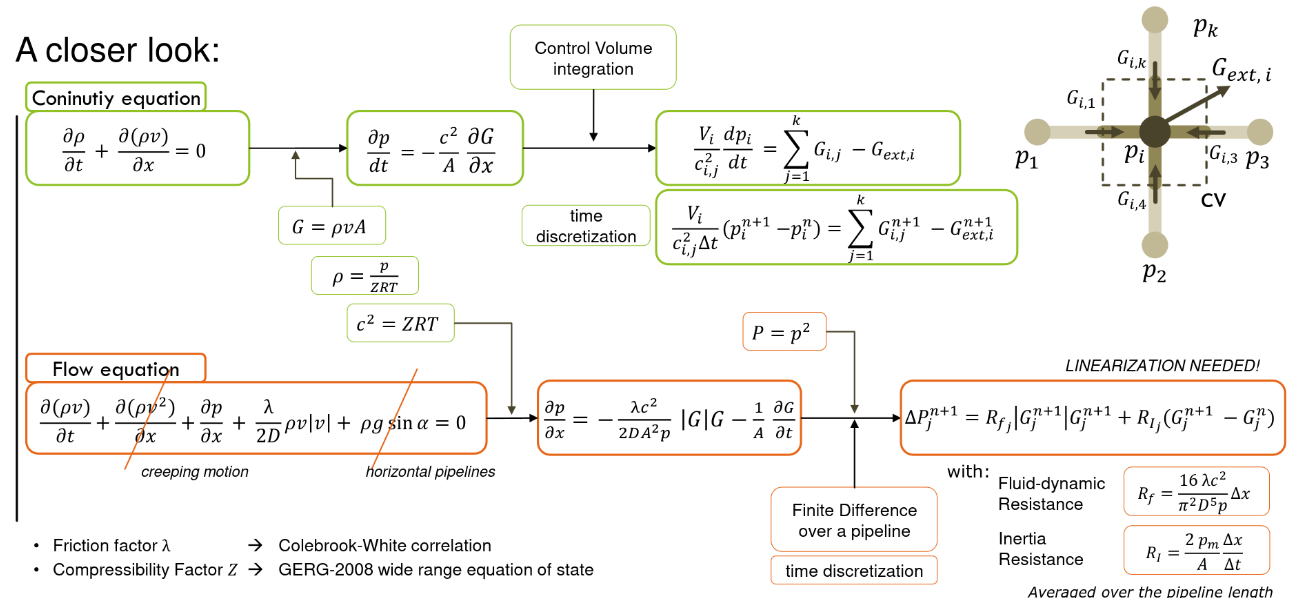
\includegraphics[scale = 1]{img_code/Marco_network_model.png}
    }};
    \node [blue, ultra thick] at ($(X.south west)!0.5!(X.north east)$) {};
    % Square for scale 0.4
    %\draw[red] (9.75,-3) -- (9.75,1.25) -- (4.0,1.25) -- (4.0,-3) -- cycle;
    % Square for scale 0.5
    \pgfsetfillcolor{lnode}
    \pgfsetfillopacity{0.5}
    \only<2->\fill(8.35,0.41) -- (8.35,1.15) -- (4.7,1.15) -- (4.7,0.41) -- cycle;
    \pgfsetfillcolor{lpipe}
    \pgfsetfillopacity{0.5}
    \only<3>\fill(7.2,-1.52) -- (7.2,-0.748) -- (11.1,-0.748) -- (11.1,-1.52) -- cycle;
    \end{tikzpicture}
    \caption{Taken from Marco's presentation.}
\end{figure}   
\end{frame}
%----------------------------------------------------------------
%----------------------------------------------------------------
\begin{frame}[fragile]{Linearized fluid-dynamic solver}

\begin{itemize}
    \item Code implementation mimics the system

\begin{minipage}{0.43\textwidth}
\begin{minted}[linenos=true,numbersep=1pt,frame=lines,framesep=2mm,fontsize=\notsotiny, escapeinside=||, bgcolor=background]{cpp}
void linearized_fluid_solver(){
 for(size_t iter=0;iter<=MAX_ITERS;iter++){    
    auto mass_system = |\cnodes{continuity}|( dt, ...);
    auto mom_system  = |\cpipes{momentum}|(dt, ...);
    auto bnd_system  = |\cbound{boundary}|(...);
        
    auto [LHS, rhs]= assemble(mass_system,
                               mom_system,
                       bnd_system, graph);

    solver.compute(LHS);
    vector_t sol = solver.solve(rhs);

    if(residual < tolerance)
       return;
 }}
\end{minted}
\end{minipage}%
\hfill
\begin{minipage}{0.45\textwidth}
    % Graphic for TeX using PGF
% Title: /home/karol/Documents/UNIVERSITA/POLITO/PRESENTATIONS/SHIMMER_2024_01/img_code/fluid_system.dia
% Creator: Dia v0.97.3
% CreationDate: Wed Jan 24 00:09:28 2024
% For: karol
% \usepackage{tikz}
% The following commands are not supported in PSTricks at present
% We define them conditionally, so when they are implemented,
% this pgf file will use them.
\ifx\du\undefined
  \newlength{\du}
\fi
\setlength{\du}{12\unitlength}
\begin{tikzpicture}[even odd rule]
\pgftransformxscale{1.000000}
\pgftransformyscale{-1.000000}
\definecolor{dialinecolor}{rgb}{0.000000, 0.000000, 0.000000}
\pgfsetstrokecolor{dialinecolor}
\pgfsetstrokeopacity{1.000000}
\definecolor{diafillcolor}{rgb}{1.000000, 1.000000, 1.000000}
\pgfsetfillcolor{diafillcolor}
\pgfsetfillopacity{1.000000}
\pgfsetlinewidth{0.050000\du}
\pgfsetdash{}{0pt}
\pgfsetmiterjoin
\pgfsetbuttcap
{\pgfsetcornersarced{\pgfpoint{0.000000\du}{0.000000\du}}\definecolor{dialinecolor}{rgb}{0.749020, 0.749020, 0.749020}
\pgfsetstrokecolor{dialinecolor}
\pgfsetstrokeopacity{1.000000}
\draw (25.200000\du,6.600000\du)--(25.200000\du,16.600000\du)--(27.500000\du,16.600000\du)--(27.500000\du,6.600000\du)--cycle;
}\pgfsetlinewidth{0.050000\du}
\pgfsetdash{}{0pt}
\pgfsetmiterjoin
\pgfsetbuttcap
{\pgfsetcornersarced{\pgfpoint{0.000000\du}{0.000000\du}}\definecolor{dialinecolor}{rgb}{0.749020, 0.749020, 0.749020}
\pgfsetstrokecolor{dialinecolor}
\pgfsetstrokeopacity{1.000000}
\draw (21.800000\du,6.600000\du)--(21.800000\du,16.600000\du)--(24.100000\du,16.600000\du)--(24.100000\du,6.600000\du)--cycle;
}\pgfsetlinewidth{0.050000\du}
\pgfsetdash{}{0pt}
\pgfsetmiterjoin
\pgfsetbuttcap
{\pgfsetcornersarced{\pgfpoint{0.000000\du}{0.000000\du}}\definecolor{dialinecolor}{rgb}{0.749020, 0.749020, 0.749020}
\pgfsetstrokecolor{dialinecolor}
\pgfsetstrokeopacity{1.000000}
\draw (11.500000\du,6.600000\du)--(11.500000\du,16.600000\du)--(21.400000\du,16.600000\du)--(21.400000\du,6.600000\du)--cycle;
}\pgfsetlinewidth{0.050000\du}
\pgfsetdash{}{0pt}
\pgfsetmiterjoin
{\pgfsetcornersarced{\pgfpoint{0.000000\du}{0.000000\du}}\definecolor{diafillcolor}{rgb}{0.882353, 0.803922, 0.882353}
\pgfsetfillcolor{lnode}
\pgfsetfillopacity{1.000000}
\fill (11.900000\du,7.000000\du)--(11.900000\du,10.000000\du)--(14.900000\du,10.000000\du)--(14.900000\du,7.000000\du)--cycle;
}{\pgfsetcornersarced{\pgfpoint{0.000000\du}{0.000000\du}}\definecolor{dialinecolor}{rgb}{0.749020, 0.749020, 0.749020}
\pgfsetstrokecolor{dialinecolor}
\pgfsetstrokeopacity{1.000000}
\draw (11.900000\du,7.000000\du)--(11.900000\du,10.000000\du)--(14.900000\du,10.000000\du)--(14.900000\du,7.000000\du)--cycle;
}% setfont left to latex
% setfont left to latex
\definecolor{dialinecolor}{rgb}{0.000000, 0.000000, 0.000000}
\pgfsetstrokecolor{dialinecolor}
\pgfsetstrokeopacity{1.000000}
\definecolor{diafillcolor}{rgb}{0.000000, 0.000000, 0.000000}
\pgfsetfillcolor{diafillcolor}
\pgfsetfillopacity{1.000000}
\node[anchor=base,inner sep=0pt, outer sep=0pt,color=dialinecolor] at (13.400000\du,8.785000\du){$\Phi$};
\pgfsetlinewidth{0.050000\du}
\pgfsetdash{}{0pt}
\pgfsetbuttcap
{
\definecolor{diafillcolor}{rgb}{0.666667, 0.670588, 0.670588}
\pgfsetfillcolor{diafillcolor}
\pgfsetfillopacity{1.000000}
% was here!!!
\definecolor{dialinecolor}{rgb}{0.666667, 0.670588, 0.670588}
\pgfsetstrokecolor{dialinecolor}
\pgfsetstrokeopacity{1.000000}
\draw (11.900000\du,7.000000\du)--(14.900000\du,10.000000\du);
}
\pgfsetlinewidth{0.050000\du}
\pgfsetdash{}{0pt}
\pgfsetmiterjoin
{\pgfsetcornersarced{\pgfpoint{0.000000\du}{0.000000\du}}\definecolor{diafillcolor}{rgb}{0.882353, 0.803922, 0.882353}
\pgfsetfillcolor{lnode}
\pgfsetfillopacity{1.000000}
\fill (15.300000\du,7.000000\du)--(15.300000\du,10.000000\du)--(17.600000\du,10.000000\du)--(17.600000\du,7.000000\du)--cycle;
}{\pgfsetcornersarced{\pgfpoint{0.000000\du}{0.000000\du}}\definecolor{dialinecolor}{rgb}{0.749020, 0.749020, 0.749020}
\pgfsetstrokecolor{dialinecolor}
\pgfsetstrokeopacity{1.000000}
\draw (15.300000\du,7.000000\du)--(15.300000\du,10.000000\du)--(17.600000\du,10.000000\du)--(17.600000\du,7.000000\du)--cycle;
}% setfont left to latex
% setfont left to latex
\definecolor{dialinecolor}{rgb}{0.000000, 0.000000, 0.000000}
\pgfsetstrokecolor{dialinecolor}
\pgfsetstrokeopacity{1.000000}
\definecolor{diafillcolor}{rgb}{0.000000, 0.000000, 0.000000}
\pgfsetfillcolor{diafillcolor}
\pgfsetfillopacity{1.000000}
\node[anchor=base,inner sep=0pt, outer sep=0pt,color=dialinecolor] at (16.450000\du,8.785000\du){$\mathbf{A}$};
\pgfsetlinewidth{0.050000\du}
\pgfsetdash{}{0pt}
\pgfsetmiterjoin
{\pgfsetcornersarced{\pgfpoint{0.000000\du}{0.000000\du}}\definecolor{diafillcolor}{rgb}{0.882353, 0.803922, 0.882353}
\pgfsetfillcolor{lnode}
\pgfsetfillopacity{1.000000}
\fill (18.000000\du,7.000000\du)--(18.000000\du,10.000000\du)--(21.000000\du,10.000000\du)--(21.000000\du,7.000000\du)--cycle;
}{\pgfsetcornersarced{\pgfpoint{0.000000\du}{0.000000\du}}\definecolor{dialinecolor}{rgb}{0.749020, 0.749020, 0.749020}
\pgfsetstrokecolor{dialinecolor}
\pgfsetstrokeopacity{1.000000}
\draw (18.000000\du,7.000000\du)--(18.000000\du,10.000000\du)--(21.000000\du,10.000000\du)--(21.000000\du,7.000000\du)--cycle;
}% setfont left to latex
% setfont left to latex
\definecolor{dialinecolor}{rgb}{0.000000, 0.000000, 0.000000}
\pgfsetstrokecolor{dialinecolor}
\pgfsetstrokeopacity{1.000000}
\definecolor{diafillcolor}{rgb}{0.000000, 0.000000, 0.000000}
\pgfsetfillcolor{diafillcolor}
\pgfsetfillopacity{1.000000}
\node[anchor=base,inner sep=0pt, outer sep=0pt,color=dialinecolor] at (19.500000\du,8.785000\du){{$\mathbf{I}$}};
\pgfsetlinewidth{0.050000\du}
\pgfsetdash{}{0pt}
\pgfsetbuttcap
{
\definecolor{diafillcolor}{rgb}{0.666667, 0.670588, 0.670588}
\pgfsetfillcolor{diafillcolor}
\pgfsetfillopacity{1.000000}
% was here!!!
\definecolor{dialinecolor}{rgb}{0.666667, 0.670588, 0.670588}
\pgfsetstrokecolor{dialinecolor}
\pgfsetstrokeopacity{1.000000}
\draw (18.000000\du,7.000000\du)--(21.000000\du,10.000000\du);
}
\pgfsetlinewidth{0.050000\du}
\pgfsetdash{}{0pt}
\pgfsetmiterjoin
{\pgfsetcornersarced{\pgfpoint{0.000000\du}{0.000000\du}}\definecolor{diafillcolor}{rgb}{0.882353, 0.803922, 0.882353}
\pgfsetfillcolor{lnode}
\pgfsetfillopacity{1.000000}
\fill (22.222183\du,7.000000\du)--(22.222183\du,10.000000\du)--(23.700000\du,10.000000\du)--(23.700000\du,7.000000\du)--cycle;
}{\pgfsetcornersarced{\pgfpoint{0.000000\du}{0.000000\du}}\definecolor{dialinecolor}{rgb}{0.749020, 0.749020, 0.749020}
\pgfsetstrokecolor{dialinecolor}
\pgfsetstrokeopacity{1.000000}
\draw (22.222183\du,7.000000\du)--(22.222183\du,10.000000\du)--(23.700000\du,10.000000\du)--(23.700000\du,7.000000\du)--cycle;
}% setfont left to latex
% setfont left to latex
\definecolor{dialinecolor}{rgb}{0.000000, 0.000000, 0.000000}
\pgfsetstrokecolor{dialinecolor}
\pgfsetstrokeopacity{1.000000}
\definecolor{diafillcolor}{rgb}{0.000000, 0.000000, 0.000000}
\pgfsetfillcolor{diafillcolor}
\pgfsetfillopacity{1.000000}
\node[anchor=base,inner sep=0pt, outer sep=0pt,color=dialinecolor] at (22.961092\du,8.785000\du){$\mathbf{p}$};
\pgfsetlinewidth{0.050000\du}
\pgfsetdash{}{0pt}
\pgfsetmiterjoin
{\pgfsetcornersarced{\pgfpoint{0.000000\du}{0.000000\du}}\definecolor{diafillcolor}{rgb}{0.882353, 0.803922, 0.882353}
\pgfsetfillcolor{lnode}
\pgfsetfillopacity{1.000000}
\fill (25.600000\du,7.000000\du)--(25.600000\du,10.000000\du)--(27.100000\du,10.000000\du)--(27.100000\du,7.000000\du)--cycle;
}{\pgfsetcornersarced{\pgfpoint{0.000000\du}{0.000000\du}}\definecolor{dialinecolor}{rgb}{0.749020, 0.749020, 0.749020}
\pgfsetstrokecolor{dialinecolor}
\pgfsetstrokeopacity{1.000000}
\draw (25.600000\du,7.000000\du)--(25.600000\du,10.000000\du)--(27.100000\du,10.000000\du)--(27.100000\du,7.000000\du)--cycle;
}% setfont left to latex
% setfont left to latex
\definecolor{dialinecolor}{rgb}{0.000000, 0.000000, 0.000000}
\pgfsetstrokecolor{dialinecolor}
\pgfsetstrokeopacity{1.000000}
\definecolor{diafillcolor}{rgb}{0.000000, 0.000000, 0.000000}
\pgfsetfillcolor{diafillcolor}
\pgfsetfillopacity{1.000000}
\node[anchor=base,inner sep=0pt, outer sep=0pt,color=dialinecolor] at (26.350000\du,8.785000\du){$\mathbf{F}_p$};
\pgfsetlinewidth{0.050000\du}
\pgfsetdash{}{0pt}
\pgfsetmiterjoin
{\pgfsetcornersarced{\pgfpoint{0.000000\du}{0.000000\du}}\definecolor{diafillcolor}{rgb}{0.847059, 0.898039, 0.898039}
\pgfsetfillcolor{lpipe}
\pgfsetfillopacity{1.000000}
\fill (11.900000\du,10.400000\du)--(11.900000\du,12.700000\du)--(14.900000\du,12.700000\du)--(14.900000\du,10.400000\du)--cycle;
}{\pgfsetcornersarced{\pgfpoint{0.000000\du}{0.000000\du}}\definecolor{dialinecolor}{rgb}{0.749020, 0.749020, 0.749020}
\pgfsetstrokecolor{dialinecolor}
\pgfsetstrokeopacity{1.000000}
\draw (11.900000\du,10.400000\du)--(11.900000\du,12.700000\du)--(14.900000\du,12.700000\du)--(14.900000\du,10.400000\du)--cycle;
}% setfont left to latex
% setfont left to latex
\definecolor{dialinecolor}{rgb}{0.000000, 0.000000, 0.000000}
\pgfsetstrokecolor{dialinecolor}
\pgfsetstrokeopacity{1.000000}
\definecolor{diafillcolor}{rgb}{0.000000, 0.000000, 0.000000}
\pgfsetfillcolor{diafillcolor}
\pgfsetfillopacity{1.000000}
\node[anchor=base,inner sep=0pt, outer sep=0pt,color=dialinecolor] at (13.400000\du,11.835000\du){$\mathbf{A}_{DP}$};
\pgfsetlinewidth{0.050000\du}
\pgfsetdash{}{0pt}
\pgfsetmiterjoin
{\pgfsetcornersarced{\pgfpoint{0.000000\du}{0.000000\du}}\definecolor{diafillcolor}{rgb}{0.847059, 0.898039, 0.898039}
\pgfsetfillcolor{lpipe}
\pgfsetfillopacity{1.000000}
\fill (15.300000\du,10.400000\du)--(15.300000\du,12.700000\du)--(17.600000\du,12.700000\du)--(17.600000\du,10.400000\du)--cycle;
}{\pgfsetcornersarced{\pgfpoint{0.000000\du}{0.000000\du}}\definecolor{dialinecolor}{rgb}{0.749020, 0.749020, 0.749020}
\pgfsetstrokecolor{dialinecolor}
\pgfsetstrokeopacity{1.000000}
\draw (15.300000\du,10.400000\du)--(15.300000\du,12.700000\du)--(17.600000\du,12.700000\du)--(17.600000\du,10.400000\du)--cycle;
}% setfont left to latex
% setfont left to latex
\definecolor{dialinecolor}{rgb}{0.000000, 0.000000, 0.000000}
\pgfsetstrokecolor{dialinecolor}
\pgfsetstrokeopacity{1.000000}
\definecolor{diafillcolor}{rgb}{0.000000, 0.000000, 0.000000}
\pgfsetfillcolor{diafillcolor}
\pgfsetfillopacity{1.000000}
\node[anchor=base,inner sep=0pt, outer sep=0pt,color=dialinecolor] at (16.450000\du,11.835000\du){{$-\mathbf{R}$}};
\pgfsetlinewidth{0.050000\du}
\pgfsetdash{}{0pt}
\pgfsetbuttcap
{
\definecolor{diafillcolor}{rgb}{0.666667, 0.670588, 0.670588}
\pgfsetfillcolor{diafillcolor}
\pgfsetfillopacity{1.000000}
% was here!!!
\definecolor{dialinecolor}{rgb}{0.666667, 0.670588, 0.670588}
\pgfsetstrokecolor{dialinecolor}
\pgfsetstrokeopacity{1.000000}
\draw (15.300000\du,10.400000\du)--(17.600000\du,12.700000\du);
}
\pgfsetlinewidth{0.050000\du}
\pgfsetdash{}{0pt}
\pgfsetmiterjoin
{\pgfsetcornersarced{\pgfpoint{0.000000\du}{0.000000\du}}\definecolor{diafillcolor}{rgb}{0.847059, 0.898039, 0.898039}
\pgfsetfillcolor{lpipe}
\pgfsetfillopacity{1.000000}
\fill (18.000000\du,10.400000\du)--(18.000000\du,12.700000\du)--(21.000000\du,12.700000\du)--(21.000000\du,10.400000\du)--cycle;
}{\pgfsetcornersarced{\pgfpoint{0.000000\du}{0.000000\du}}\definecolor{dialinecolor}{rgb}{0.749020, 0.749020, 0.749020}
\pgfsetstrokecolor{dialinecolor}
\pgfsetstrokeopacity{1.000000}
\draw (18.000000\du,10.400000\du)--(18.000000\du,12.700000\du)--(21.000000\du,12.700000\du)--(21.000000\du,10.400000\du)--cycle;
}% setfont left to latex
% setfont left to latex
\definecolor{dialinecolor}{rgb}{0.000000, 0.000000, 0.000000}
\pgfsetstrokecolor{dialinecolor}
\pgfsetstrokeopacity{1.000000}
\definecolor{diafillcolor}{rgb}{0.000000, 0.000000, 0.000000}
\pgfsetfillcolor{diafillcolor}
\pgfsetfillopacity{1.000000}
\node[anchor=base,inner sep=0pt, outer sep=0pt,color=dialinecolor] at (19.500000\du,11.835000\du){{$\mathbf{0}$}};
\pgfsetlinewidth{0.050000\du}
\pgfsetdash{}{0pt}
\pgfsetmiterjoin
{\pgfsetcornersarced{\pgfpoint{0.000000\du}{0.000000\du}}\definecolor{diafillcolor}{rgb}{0.847059, 0.898039, 0.898039}
\pgfsetfillcolor{lpipe}
\pgfsetfillopacity{1.000000}
\fill (22.222183\du,10.400000\du)--(22.222183\du,12.700000\du)--(23.700000\du,12.700000\du)--(23.700000\du,10.400000\du)--cycle;
}{\pgfsetcornersarced{\pgfpoint{0.000000\du}{0.000000\du}}\definecolor{dialinecolor}{rgb}{0.749020, 0.749020, 0.749020}
\pgfsetstrokecolor{dialinecolor}
\pgfsetstrokeopacity{1.000000}
\draw (22.222183\du,10.400000\du)--(22.222183\du,12.700000\du)--(23.700000\du,12.700000\du)--(23.700000\du,10.400000\du)--cycle;
}% setfont left to latex
% setfont left to latex
\definecolor{dialinecolor}{rgb}{0.000000, 0.000000, 0.000000}
\pgfsetstrokecolor{dialinecolor}
\pgfsetstrokeopacity{1.000000}
\definecolor{diafillcolor}{rgb}{0.000000, 0.000000, 0.000000}
\pgfsetfillcolor{diafillcolor}
\pgfsetfillopacity{1.000000}
\node[anchor=base,inner sep=0pt, outer sep=0pt,color=dialinecolor] at (22.961092\du,11.835000\du){$\mathbf{G}$};
\pgfsetlinewidth{0.050000\du}
\pgfsetdash{}{0pt}
\pgfsetmiterjoin
{\pgfsetcornersarced{\pgfpoint{0.000000\du}{0.000000\du}}\definecolor{diafillcolor}{rgb}{0.847059, 0.898039, 0.898039}
\pgfsetfillcolor{lpipe}
\pgfsetfillopacity{1.000000}
\fill (25.600000\du,10.400000\du)--(25.600000\du,12.700000\du)--(27.100000\du,12.700000\du)--(27.100000\du,10.400000\du)--cycle;
}{\pgfsetcornersarced{\pgfpoint{0.000000\du}{0.000000\du}}\definecolor{dialinecolor}{rgb}{0.749020, 0.749020, 0.749020}
\pgfsetstrokecolor{dialinecolor}
\pgfsetstrokeopacity{1.000000}
\draw (25.600000\du,10.400000\du)--(25.600000\du,12.700000\du)--(27.100000\du,12.700000\du)--(27.100000\du,10.400000\du)--cycle;
}% setfont left to latex
% setfont left to latex
\definecolor{dialinecolor}{rgb}{0.000000, 0.000000, 0.000000}
\pgfsetstrokecolor{dialinecolor}
\pgfsetstrokeopacity{1.000000}
\definecolor{diafillcolor}{rgb}{1.000000, 1.000000, 1.000000}
\pgfsetfillcolor{diafillcolor}
\pgfsetfillopacity{1.000000}
\node[anchor=base,inner sep=0pt, outer sep=0pt,color=dialinecolor] at (26.350000\du,11.835000\du){$\mathbf{F}_G$};
\pgfsetlinewidth{0.050000\du}
\pgfsetdash{}{0pt}
\pgfsetmiterjoin
{\pgfsetcornersarced{\pgfpoint{0.000000\du}{0.000000\du}}\definecolor{diafillcolor}{rgb}{0.882353, 0.825071, 0.686107}
\pgfsetfillcolor{lbound}
\pgfsetfillopacity{1.000000}
\fill (11.900000\du,13.200000\du)--(11.900000\du,16.200000\du)--(14.900000\du,16.200000\du)--(14.900000\du,13.200000\du)--cycle;
}{\pgfsetcornersarced{\pgfpoint{0.000000\du}{0.000000\du}}\definecolor{dialinecolor}{rgb}{0.749020, 0.749020, 0.749020}
\pgfsetstrokecolor{dialinecolor}
\pgfsetstrokeopacity{1.000000}
\draw (11.900000\du,13.200000\du)--(11.900000\du,16.200000\du)--(14.900000\du,16.200000\du)--(14.900000\du,13.200000\du)--cycle;
}% setfont left to latex
% setfont left to latex
\definecolor{dialinecolor}{rgb}{0.000000, 0.000000, 0.000000}
\pgfsetstrokecolor{dialinecolor}
\pgfsetstrokeopacity{1.000000}
\definecolor{diafillcolor}{rgb}{0.000000, 0.000000, 0.000000}
\pgfsetfillcolor{diafillcolor}
\pgfsetfillopacity{1.000000}
\node[anchor=base,inner sep=0pt, outer sep=0pt,color=dialinecolor] at (13.400000\du,14.985000\du){};
\pgfsetlinewidth{0.100000\du}
\pgfsetdash{{\pgflinewidth}{0.200000\du}}{0cm}
\pgfsetbuttcap
{
\definecolor{diafillcolor}{rgb}{0.666667, 0.670588, 0.670588}
\pgfsetfillcolor{diafillcolor}
\pgfsetfillopacity{1.000000}
% was here!!!
\definecolor{dialinecolor}{rgb}{0.666667, 0.670588, 0.670588}
\pgfsetstrokecolor{dialinecolor}
\pgfsetstrokeopacity{1.000000}
\draw (11.900000\du,13.200000\du)--(14.900000\du,16.200000\du);
}
\pgfsetlinewidth{0.050000\du}
\pgfsetdash{}{0pt}
\pgfsetmiterjoin
{\pgfsetcornersarced{\pgfpoint{0.000000\du}{0.000000\du}}\definecolor{diafillcolor}{rgb}{0.882353, 0.825071, 0.686107}
\pgfsetfillcolor{lbound}
\pgfsetfillopacity{1.000000}
\fill (15.300000\du,13.200000\du)--(15.300000\du,16.200000\du)--(17.600000\du,16.200000\du)--(17.600000\du,13.200000\du)--cycle;
}{\pgfsetcornersarced{\pgfpoint{0.000000\du}{0.000000\du}}\definecolor{dialinecolor}{rgb}{0.749020, 0.749020, 0.749020}
\pgfsetstrokecolor{dialinecolor}
\pgfsetstrokeopacity{1.000000}
\draw (15.300000\du,13.200000\du)--(15.300000\du,16.200000\du)--(17.600000\du,16.200000\du)--(17.600000\du,13.200000\du)--cycle;
}% setfont left to latex
% setfont left to latex
\definecolor{dialinecolor}{rgb}{0.000000, 0.000000, 0.000000}
\pgfsetstrokecolor{dialinecolor}
\pgfsetstrokeopacity{1.000000}
\definecolor{diafillcolor}{rgb}{0.000000, 0.000000, 0.000000}
\pgfsetfillcolor{diafillcolor}
\pgfsetfillopacity{1.000000}
\node[anchor=base,inner sep=0pt, outer sep=0pt,color=dialinecolor] at (16.450000\du,14.985000\du){$\mathbf{0}$};
\pgfsetlinewidth{0.050000\du}
\pgfsetdash{}{0pt}
\pgfsetmiterjoin
{\pgfsetcornersarced{\pgfpoint{0.000000\du}{0.000000\du}}\definecolor{diafillcolor}{rgb}{0.882353, 0.825071, 0.686107}
\pgfsetfillcolor{lbound}
\pgfsetfillopacity{1.000000}
\fill (18.000000\du,13.200000\du)--(18.000000\du,16.200000\du)--(21.000000\du,16.200000\du)--(21.000000\du,13.200000\du)--cycle;
}{\pgfsetcornersarced{\pgfpoint{0.000000\du}{0.000000\du}}\definecolor{dialinecolor}{rgb}{0.749020, 0.749020, 0.749020}
\pgfsetstrokecolor{dialinecolor}
\pgfsetstrokeopacity{1.000000}
\draw (18.000000\du,13.200000\du)--(18.000000\du,16.200000\du)--(21.000000\du,16.200000\du)--(21.000000\du,13.200000\du)--cycle;
}% setfont left to latex
% setfont left to latex
\definecolor{dialinecolor}{rgb}{0.000000, 0.000000, 0.000000}
\pgfsetstrokecolor{dialinecolor}
\pgfsetstrokeopacity{1.000000}
\definecolor{diafillcolor}{rgb}{0.000000, 0.000000, 0.000000}
\pgfsetfillcolor{diafillcolor}
\pgfsetfillopacity{1.000000}
\node[anchor=base,inner sep=0pt, outer sep=0pt,color=dialinecolor] at (19.500000\du,14.985000\du){};
\pgfsetlinewidth{0.100000\du}
\pgfsetdash{{\pgflinewidth}{0.200000\du}}{0cm}
\pgfsetbuttcap
{
\definecolor{diafillcolor}{rgb}{0.666667, 0.670588, 0.670588}
\pgfsetfillcolor{diafillcolor}
\pgfsetfillopacity{1.000000}
% was here!!!
\definecolor{dialinecolor}{rgb}{0.666667, 0.670588, 0.670588}
\pgfsetstrokecolor{dialinecolor}
\pgfsetstrokeopacity{1.000000}
\draw (18.000000\du,13.200000\du)--(21.000000\du,16.200000\du);
}
\pgfsetlinewidth{0.050000\du}
\pgfsetdash{}{0pt}
\pgfsetmiterjoin
{\pgfsetcornersarced{\pgfpoint{0.000000\du}{0.000000\du}}\definecolor{diafillcolor}{rgb}{0.882353, 0.825071, 0.686107}
\pgfsetfillcolor{lbound}
\pgfsetfillopacity{1.000000}
\fill (22.222183\du,13.200000\du)--(22.222183\du,16.200000\du)--(23.700000\du,16.200000\du)--(23.700000\du,13.200000\du)--cycle;
}{\pgfsetcornersarced{\pgfpoint{0.000000\du}{0.000000\du}}\definecolor{dialinecolor}{rgb}{0.749020, 0.749020, 0.749020}
\pgfsetstrokecolor{dialinecolor}
\pgfsetstrokeopacity{1.000000}
\draw (22.222183\du,13.200000\du)--(22.222183\du,16.200000\du)--(23.700000\du,16.200000\du)--(23.700000\du,13.200000\du)--cycle;
}% setfont left to latex
% setfont left to latex
\definecolor{dialinecolor}{rgb}{0.000000, 0.000000, 0.000000}
\pgfsetstrokecolor{dialinecolor}
\pgfsetstrokeopacity{1.000000}
\definecolor{diafillcolor}{rgb}{0.000000, 0.000000, 0.000000}
\pgfsetfillcolor{diafillcolor}
\pgfsetfillopacity{1.000000}
\node[anchor=base,inner sep=0pt, outer sep=0pt,color=dialinecolor] at (22.961092\du,14.985000\du){$\mathbf{L}$};
\pgfsetlinewidth{0.050000\du}
\pgfsetdash{}{0pt}
\pgfsetmiterjoin
{\pgfsetcornersarced{\pgfpoint{0.000000\du}{0.000000\du}}\definecolor{diafillcolor}{rgb}{0.882353, 0.825071, 0.686107}
\pgfsetfillcolor{lbound}
\pgfsetfillopacity{1.000000}
\fill (25.600000\du,13.200000\du)--(25.600000\du,16.200000\du)--(27.100000\du,16.200000\du)--(27.100000\du,13.200000\du)--cycle;
}{\pgfsetcornersarced{\pgfpoint{0.000000\du}{0.000000\du}}\definecolor{dialinecolor}{rgb}{0.749020, 0.749020, 0.749020}
\pgfsetstrokecolor{dialinecolor}
\pgfsetstrokeopacity{1.000000}
\draw (25.600000\du,13.200000\du)--(25.600000\du,16.200000\du)--(27.100000\du,16.200000\du)--(27.100000\du,13.200000\du)--cycle;
}% setfont left to latex
% setfont left to latex
\definecolor{dialinecolor}{rgb}{0.000000, 0.000000, 0.000000}
\pgfsetstrokecolor{dialinecolor}
\pgfsetstrokeopacity{1.000000}
\definecolor{diafillcolor}{rgb}{0.000000, 0.000000, 0.000000}
\pgfsetfillcolor{diafillcolor}
\pgfsetfillopacity{1.000000}
\node[anchor=base,inner sep=0pt, outer sep=0pt,color=dialinecolor] at (26.350000\du,14.985000\du){$\mathbf{F}_b$};
% setfont left to latex
% setfont left to latex
\definecolor{dialinecolor}{rgb}{0.000000, 0.000000, 0.000000}
\pgfsetstrokecolor{dialinecolor}
\pgfsetstrokeopacity{1.000000}
\definecolor{diafillcolor}{rgb}{0.000000, 0.000000, 0.000000}
\pgfsetfillcolor{diafillcolor}
\pgfsetfillopacity{1.000000}
\node[anchor=base west,inner sep=0pt,outer sep=0pt,color=dialinecolor] at (24.400000\du,11.900000\du){=};
\pgfsetlinewidth{0.050000\du}
\pgfsetdash{}{0pt}
\pgfsetmiterjoin
{\pgfsetcornersarced{\pgfpoint{0.000000\du}{0.000000\du}}\definecolor{diafillcolor}{rgb}{0.898039, 0.898039, 0.898039}
\pgfsetfillcolor{diafillcolor}
\pgfsetfillopacity{1.000000}
\fill (28.054032\du,17.267559\du)--(28.054032\du,18.267559\du)--(29.054032\du,18.267559\du)--(29.054032\du,17.267559\du)--cycle;
}{\pgfsetcornersarced{\pgfpoint{0.000000\du}{0.000000\du}}\definecolor{dialinecolor}{rgb}{0.749020, 0.749020, 0.749020}
\pgfsetstrokecolor{dialinecolor}
\pgfsetstrokeopacity{1.000000}
\draw (28.054032\du,17.267559\du)--(28.054032\du,18.267559\du)--(29.054032\du,18.267559\du)--(29.054032\du,17.267559\du)--cycle;
}% setfont left to latex
% setfont left to latex
\definecolor{dialinecolor}{rgb}{0.000000, 0.000000, 0.000000}
\pgfsetstrokecolor{dialinecolor}
\pgfsetstrokeopacity{1.000000}
\definecolor{diafillcolor}{rgb}{0.000000, 0.000000, 0.000000}
\pgfsetfillcolor{diafillcolor}
\pgfsetfillopacity{1.000000}
\node[anchor=base,inner sep=0pt, outer sep=0pt,color=dialinecolor] at (22.554032\du,18.052559\du){};
\pgfsetlinewidth{0.050000\du}
\pgfsetdash{}{0pt}
\pgfsetbuttcap
{
\definecolor{diafillcolor}{rgb}{0.666667, 0.670588, 0.670588}
\pgfsetfillcolor{diafillcolor}
\pgfsetfillopacity{1.000000}
% was here!!!
\definecolor{dialinecolor}{rgb}{0.666667, 0.670588, 0.670588}
\pgfsetstrokecolor{dialinecolor}
\pgfsetstrokeopacity{1.000000}
\draw (28.054032\du,17.267559\du)--(29.054032\du,18.267559\du);
}
% setfont left to latex
% setfont left to latex
\definecolor{dialinecolor}{rgb}{0.000000, 0.000000, 0.000000}
\pgfsetstrokecolor{dialinecolor}
\pgfsetstrokeopacity{1.000000}
\definecolor{diafillcolor}{rgb}{0.000000, 0.000000, 0.000000}
\pgfsetfillcolor{diafillcolor}
\pgfsetfillopacity{1.000000}
\node[anchor=base west,inner sep=0pt,outer sep=0pt,color=dialinecolor] at (21.00000\du,18.000000\du){Diagonal matrix};
\end{tikzpicture}

\end{minipage}

\item Functions parameters:
\begin{minted}[linenos=true,numbersep=1pt,frame=lines,framesep=2mm,fontsize=\notsotiny,escapeinside=||, bgcolor=background]{cpp}
     |\cnodes{continuity}|( dt, Tm, pressure, pressure_old, incidence, graph, x_nodes, glaw_nodes);
     |\cpipes{momentum}|( dt, Tm, flux, flux_old, pressure, incidence, graph, x_pipes, glaw_pipes);
     |\cbound{boundary}|(p_in, vel, flux_ext, incidence, graph, inlet_nodes);
\end{minted}
\end{itemize}
\end{frame}
%----------------------------------------------------------------
%----------------------------------------------------------------
\begin{frame}[fragile]{Modified incidence matrix $\mathbf{A}_{DP}$}
\noindent
\begin{itemize}
    \setlength{\itemindent}{-2.em}
    \item Linearized momentum equation
    \begin{equation*}
        \fbox{$P_{j,in}^{k+1} - e^sP_{j,out}^{n+1}$} - (2R^k_{F,j}|G_j^{k}| + R_{I,j}) G_j^{k+1} = F_G(R_{I},R^k_F,G_j^{k})
    \end{equation*}
\end{itemize}

\begin{minipage}{0.465\textwidth}
with matrix form
\begin{center}
% Graphic for TeX using PGF
% Title: /home/karol/Documents/UNIVERSITA/POLITO/PRESENTATIONS/SHIMMER_2024_01/img_code/fluid_system_momentum_adp.dia
% Creator: Dia v0.97.3
% CreationDate: Wed Jan 24 15:42:32 2024
% For: karol
% \usepackage{tikz}
% The following commands are not supported in PSTricks at present
% We define them conditionally, so when they are implemented,
% this pgf file will use them.
\ifx\du\undefined
  \newlength{\du}
\fi
\setlength{\du}{10\unitlength}
\begin{tikzpicture}[even odd rule]
\pgftransformxscale{1.000000}
\pgftransformyscale{-1.000000}
\definecolor{dialinecolor}{rgb}{0.000000, 0.000000, 0.000000}
\pgfsetstrokecolor{dialinecolor}
\pgfsetstrokeopacity{1.000000}
\definecolor{diafillcolor}{rgb}{1.000000, 1.000000, 1.000000}
\pgfsetfillcolor{diafillcolor}
\pgfsetfillopacity{1.000000}
\pgfsetlinewidth{0.050000\du}
\pgfsetdash{}{0pt}
\pgfsetmiterjoin
{\pgfsetcornersarced{\pgfpoint{0.000000\du}{0.000000\du}}\definecolor{diafillcolor}{rgb}{0.882353, 0.803922, 0.882353}
\pgfsetfillcolor{diafillcolor}
\pgfsetfillopacity{1.000000}
\fill (12.400000\du,5.000000\du)--(12.400000\du,8.000000\du)--(13.877817\du,8.000000\du)--(13.877817\du,5.000000\du)--cycle;
}{\pgfsetcornersarced{\pgfpoint{0.000000\du}{0.000000\du}}\definecolor{dialinecolor}{rgb}{0.749020, 0.749020, 0.749020}
\pgfsetstrokecolor{dialinecolor}
\pgfsetstrokeopacity{1.000000}
\draw (12.400000\du,5.000000\du)--(12.400000\du,8.000000\du)--(13.877817\du,8.000000\du)--(13.877817\du,5.000000\du)--cycle;
}% setfont left to latex
% setfont left to latex
\definecolor{dialinecolor}{rgb}{0.000000, 0.000000, 0.000000}
\pgfsetstrokecolor{dialinecolor}
\pgfsetstrokeopacity{1.000000}
\definecolor{diafillcolor}{rgb}{0.000000, 0.000000, 0.000000}
\pgfsetfillcolor{diafillcolor}
\pgfsetfillopacity{1.000000}
\node[anchor=base,inner sep=0pt, outer sep=0pt,color=dialinecolor] at (13.138908\du,6.785000\du){$\mathbf{p}$};
\pgfsetlinewidth{0.050000\du}
\pgfsetdash{}{0pt}
\pgfsetmiterjoin
{\pgfsetcornersarced{\pgfpoint{0.000000\du}{0.000000\du}}\definecolor{diafillcolor}{rgb}{0.847059, 0.898039, 0.898039}
\pgfsetfillcolor{diafillcolor}
\pgfsetfillopacity{1.000000}
\fill (9.000000\du,5.000000\du)--(9.000000\du,7.300000\du)--(12.000000\du,7.300000\du)--(12.000000\du,5.000000\du)--cycle;
}{\pgfsetcornersarced{\pgfpoint{0.000000\du}{0.000000\du}}\definecolor{dialinecolor}{rgb}{1.000000, 0.000000, 0.000000}
\pgfsetstrokecolor{dialinecolor}
\pgfsetstrokeopacity{1.000000}
\draw (9.000000\du,5.000000\du)--(9.000000\du,7.300000\du)--(12.000000\du,7.300000\du)--(12.000000\du,5.000000\du)--cycle;
}% setfont left to latex
% setfont left to latex
\definecolor{dialinecolor}{rgb}{0.000000, 0.000000, 0.000000}
\pgfsetstrokecolor{dialinecolor}
\pgfsetstrokeopacity{1.000000}
\definecolor{diafillcolor}{rgb}{0.000000, 0.000000, 0.000000}
\pgfsetfillcolor{diafillcolor}
\pgfsetfillopacity{1.000000}
\node[anchor=base,inner sep=0pt, outer sep=0pt,color=dialinecolor] at (10.500000\du,6.435000\du){$\mathbf{A}_{DP}$};
\pgfsetlinewidth{0.050000\du}
\pgfsetdash{}{0pt}
\pgfsetmiterjoin
{\pgfsetcornersarced{\pgfpoint{0.000000\du}{0.000000\du}}\definecolor{diafillcolor}{rgb}{0.847059, 0.898039, 0.898039}
\pgfsetfillcolor{diafillcolor}
\pgfsetfillopacity{1.000000}
\fill (14.600000\du,5.000000\du)--(14.600000\du,7.300000\du)--(16.900000\du,7.300000\du)--(16.900000\du,5.000000\du)--cycle;
}{\pgfsetcornersarced{\pgfpoint{0.000000\du}{0.000000\du}}\definecolor{dialinecolor}{rgb}{0.749020, 0.749020, 0.749020}
\pgfsetstrokecolor{dialinecolor}
\pgfsetstrokeopacity{1.000000}
\draw (14.600000\du,5.000000\du)--(14.600000\du,7.300000\du)--(16.900000\du,7.300000\du)--(16.900000\du,5.000000\du)--cycle;
}% setfont left to latex
% setfont left to latex
\definecolor{dialinecolor}{rgb}{0.000000, 0.000000, 0.000000}
\pgfsetstrokecolor{dialinecolor}
\pgfsetstrokeopacity{1.000000}
\definecolor{diafillcolor}{rgb}{0.000000, 0.000000, 0.000000}
\pgfsetfillcolor{diafillcolor}
\pgfsetfillopacity{1.000000}
\node[anchor=base,inner sep=0pt, outer sep=0pt,color=dialinecolor] at (15.750000\du,6.435000\du){$\mathbf{R}$};
\pgfsetlinewidth{0.050000\du}
\pgfsetdash{}{0pt}
\pgfsetbuttcap
{
\definecolor{diafillcolor}{rgb}{0.666667, 0.670588, 0.670588}
\pgfsetfillcolor{diafillcolor}
\pgfsetfillopacity{1.000000}
% was here!!!
\definecolor{dialinecolor}{rgb}{0.666667, 0.670588, 0.670588}
\pgfsetstrokecolor{dialinecolor}
\pgfsetstrokeopacity{1.000000}
\draw (14.600000\du,5.000000\du)--(16.900000\du,7.300000\du);
}
\pgfsetlinewidth{0.050000\du}
\pgfsetdash{}{0pt}
\pgfsetmiterjoin
{\pgfsetcornersarced{\pgfpoint{0.000000\du}{0.000000\du}}\definecolor{diafillcolor}{rgb}{0.847059, 0.898039, 0.898039}
\pgfsetfillcolor{diafillcolor}
\pgfsetfillopacity{1.000000}
\fill (17.300000\du,5.000000\du)--(17.300000\du,7.300000\du)--(18.777817\du,7.300000\du)--(18.777817\du,5.000000\du)--cycle;
}{\pgfsetcornersarced{\pgfpoint{0.000000\du}{0.000000\du}}\definecolor{dialinecolor}{rgb}{0.749020, 0.749020, 0.749020}
\pgfsetstrokecolor{dialinecolor}
\pgfsetstrokeopacity{1.000000}
\draw (17.300000\du,5.000000\du)--(17.300000\du,7.300000\du)--(18.777817\du,7.300000\du)--(18.777817\du,5.000000\du)--cycle;
}% setfont left to latex
% setfont left to latex
\definecolor{dialinecolor}{rgb}{0.000000, 0.000000, 0.000000}
\pgfsetstrokecolor{dialinecolor}
\pgfsetstrokeopacity{1.000000}
\definecolor{diafillcolor}{rgb}{0.000000, 0.000000, 0.000000}
\pgfsetfillcolor{diafillcolor}
\pgfsetfillopacity{1.000000}
\node[anchor=base,inner sep=0pt, outer sep=0pt,color=dialinecolor] at (18.038908\du,6.435000\du){$\mathbf{G}$};
\pgfsetlinewidth{0.050000\du}
\pgfsetdash{}{0pt}
\pgfsetmiterjoin
{\pgfsetcornersarced{\pgfpoint{0.000000\du}{0.000000\du}}\definecolor{diafillcolor}{rgb}{0.847059, 0.898039, 0.898039}
\pgfsetfillcolor{diafillcolor}
\pgfsetfillopacity{1.000000}
\fill (19.500000\du,5.000000\du)--(19.500000\du,7.300000\du)--(21.000000\du,7.300000\du)--(21.000000\du,5.000000\du)--cycle;
}{\pgfsetcornersarced{\pgfpoint{0.000000\du}{0.000000\du}}\definecolor{dialinecolor}{rgb}{0.749020, 0.749020, 0.749020}
\pgfsetstrokecolor{dialinecolor}
\pgfsetstrokeopacity{1.000000}
\draw (19.500000\du,5.000000\du)--(19.500000\du,7.300000\du)--(21.000000\du,7.300000\du)--(21.000000\du,5.000000\du)--cycle;
}% setfont left to latex
% setfont left to latex
\definecolor{dialinecolor}{rgb}{0.000000, 0.000000, 0.000000}
\pgfsetstrokecolor{dialinecolor}
\pgfsetstrokeopacity{1.000000}
\definecolor{diafillcolor}{rgb}{0.000000, 0.000000, 0.000000}
\pgfsetfillcolor{diafillcolor}
\pgfsetfillopacity{1.000000}
\node[anchor=base,inner sep=0pt, outer sep=0pt,color=dialinecolor] at (20.250000\du,6.435000\du){$\mathbf{F_G}$};
% setfont left to latex
% setfont left to latex
\definecolor{dialinecolor}{rgb}{0.000000, 0.000000, 0.000000}
\pgfsetstrokecolor{dialinecolor}
\pgfsetstrokeopacity{1.000000}
\definecolor{diafillcolor}{rgb}{0.000000, 0.000000, 0.000000}
\pgfsetfillcolor{diafillcolor}
\pgfsetfillopacity{1.000000}
\node[anchor=base west,inner sep=0pt,outer sep=0pt,color=dialinecolor] at (18.8000000\du,6.300000\du){=};
% setfont left to latex
% setfont left to latex
\definecolor{dialinecolor}{rgb}{0.000000, 0.000000, 0.000000}
\pgfsetstrokecolor{dialinecolor}
\pgfsetstrokeopacity{1.000000}
\definecolor{diafillcolor}{rgb}{0.000000, 0.000000, 0.000000}
\pgfsetfillcolor{diafillcolor}
\pgfsetfillopacity{1.000000}
\node[anchor=base west,inner sep=0pt,outer sep=0pt,color=dialinecolor] at (13.961341\du,6.306816\du){-};
\end{tikzpicture}
     
\end{center}
\vspace{-0.5cm}
\begin{minted}[linenos=true,numbersep=1pt,frame=lines,framesep=2mm,fontsize=\notsotiny, bgcolor=background]{cpp}
smatrix_t
adp_matrix( const vector_t& c2, const my_graph& g,
            const incidence& inc)
{ 
   vector_t  exp_s = compute_expS(c2, g);
   smatrix_t sE = diag_matrix(exp_s);  

   smatrix_t ADP(num_edges(g),num_vertices(g));
   ADPt = inc.matrix_in() - inc.matrix_out()*sE;
   return ADPt.transpose();
}    
\end{minted}    
\end{minipage}
\hfill
\begin{minipage}{0.47\textwidth}
    \begin{minted}[linenos=true,numbersep=1pt,frame=lines,framesep=2mm,fontsize=\notsotiny, bgcolor=background]{cpp}
vector_t
compute_expS(const vector_t& c2, const my_graph& g)
{   
    vector_t  exp_s (num_edges(g)); 

    size_t i = 0;
    auto r = edges(g);
    for(auto it=r.first; it!=r.second; it++,i++)
    {
        auto pipe = g[*it];   
        auto node_in  = g[source(*it, g)];
        auto node_out = g[target(*it, g)];
        auto s = node_out.height - node_in.height;
        exp_s(i) =  std::exp(s * gravity / c2(i)); 
    }

    return exp_s;       
}
    \end{minted}
\end{minipage}
 \begin{tikzpicture}[remember picture,overlay]
\only<2>\draw[red] (-13.7,-1.56) -- (-13.7,-1.32) -- (-7.5,-1.32) -- (-7.5,-1.56) -- cycle;
 \end{tikzpicture}
\end{frame}
%----------------------------------------------------------------
%----------------------------------------------------------------

\begin{frame}[fragile]{Resistance matrix}
\noindent
%\hspace{-0.5cm}
\begin{minipage}{0.45\textwidth}
\begin{itemize}
    \setlength{\itemindent}{-2.em}
    \item Linearized momentum equation
\end{itemize}
    \noindent \hspace{-0.5cm}
    \[\small
        P_{j,in}^{k+1} - e^sP_{j,out}^{n+1} -\fbox{$(2R^k_{F,j}|G_j^{k}| + R_{I,j})$} G_j^{k+1} = F_G
    \]
    with matrix form 
    \begin{center}
    % Graphic for TeX using PGF
% Title: /home/karol/Documents/UNIVERSITA/POLITO/PRESENTATIONS/SHIMMER_2024_01/img_code/fluid_system_momentum_adp.dia
% Creator: Dia v0.97.3
% CreationDate: Thu Jan 25 10:36:14 2024
% For: karol
% \usepackage{tikz}
% The following commands are not supported in PSTricks at present
% We define them conditionally, so when they are implemented,
% this pgf file will use them.
\ifx\du\undefined
  \newlength{\du}
\fi
\setlength{\du}{10\unitlength}
\begin{tikzpicture}[even odd rule]
\pgftransformxscale{1.000000}
\pgftransformyscale{-1.000000}
\definecolor{dialinecolor}{rgb}{0.000000, 0.000000, 0.000000}
\pgfsetstrokecolor{dialinecolor}
\pgfsetstrokeopacity{1.000000}
\definecolor{diafillcolor}{rgb}{1.000000, 1.000000, 1.000000}
\pgfsetfillcolor{diafillcolor}
\pgfsetfillopacity{1.000000}
\pgfsetlinewidth{0.050000\du}
\pgfsetdash{}{0pt}
\pgfsetmiterjoin
{\pgfsetcornersarced{\pgfpoint{0.000000\du}{0.000000\du}}\definecolor{diafillcolor}{rgb}{0.882353, 0.803922, 0.882353}
\pgfsetfillcolor{diafillcolor}
\pgfsetfillopacity{1.000000}
\fill (12.400000\du,5.000000\du)--(12.400000\du,8.000000\du)--(13.877817\du,8.000000\du)--(13.877817\du,5.000000\du)--cycle;
}{\pgfsetcornersarced{\pgfpoint{0.000000\du}{0.000000\du}}\definecolor{dialinecolor}{rgb}{0.749020, 0.749020, 0.749020}
\pgfsetstrokecolor{dialinecolor}
\pgfsetstrokeopacity{1.000000}
\draw (12.400000\du,5.000000\du)--(12.400000\du,8.000000\du)--(13.877817\du,8.000000\du)--(13.877817\du,5.000000\du)--cycle;
}% setfont left to latex
% setfont left to latex
\definecolor{dialinecolor}{rgb}{0.000000, 0.000000, 0.000000}
\pgfsetstrokecolor{dialinecolor}
\pgfsetstrokeopacity{1.000000}
\definecolor{diafillcolor}{rgb}{0.000000, 0.000000, 0.000000}
\pgfsetfillcolor{diafillcolor}
\pgfsetfillopacity{1.000000}
\node[anchor=base,inner sep=0pt, outer sep=0pt,color=dialinecolor] at (13.138908\du,6.785000\du){$\mathbf{p}$};
\pgfsetlinewidth{0.050000\du}
\pgfsetdash{}{0pt}
\pgfsetmiterjoin
{\pgfsetcornersarced{\pgfpoint{0.000000\du}{0.000000\du}}\definecolor{diafillcolor}{rgb}{0.847059, 0.898039, 0.898039}
\pgfsetfillcolor{diafillcolor}
\pgfsetfillopacity{1.000000}
\fill (9.000000\du,5.000000\du)--(9.000000\du,7.300000\du)--(12.000000\du,7.300000\du)--(12.000000\du,5.000000\du)--cycle;
}{\pgfsetcornersarced{\pgfpoint{0.000000\du}{0.000000\du}}\definecolor{dialinecolor}{rgb}{0.666667, 0.670588, 0.670588}
\pgfsetstrokecolor{dialinecolor}
\pgfsetstrokeopacity{1.000000}
\draw (9.000000\du,5.000000\du)--(9.000000\du,7.300000\du)--(12.000000\du,7.300000\du)--(12.000000\du,5.000000\du)--cycle;
}% setfont left to latex
% setfont left to latex
\definecolor{dialinecolor}{rgb}{0.000000, 0.000000, 0.000000}
\pgfsetstrokecolor{dialinecolor}
\pgfsetstrokeopacity{1.000000}
\definecolor{diafillcolor}{rgb}{0.000000, 0.000000, 0.000000}
\pgfsetfillcolor{diafillcolor}
\pgfsetfillopacity{1.000000}
\node[anchor=base,inner sep=0pt, outer sep=0pt,color=dialinecolor] at (10.500000\du,6.435000\du){$\mathbf{A}_{DP}$};
\pgfsetlinewidth{0.050000\du}
\pgfsetdash{}{0pt}
\pgfsetmiterjoin
{\pgfsetcornersarced{\pgfpoint{0.000000\du}{0.000000\du}}\definecolor{diafillcolor}{rgb}{0.847059, 0.898039, 0.898039}
\pgfsetfillcolor{diafillcolor}
\pgfsetfillopacity{1.000000}
\fill (14.600000\du,5.000000\du)--(14.600000\du,7.300000\du)--(16.900000\du,7.300000\du)--(16.900000\du,5.000000\du)--cycle;
}{\pgfsetcornersarced{\pgfpoint{0.000000\du}{0.000000\du}}\definecolor{dialinecolor}{rgb}{1.000000, 0.000000, 0.000000}
\pgfsetstrokecolor{dialinecolor}
\pgfsetstrokeopacity{1.000000}
\draw (14.600000\du,5.000000\du)--(14.600000\du,7.300000\du)--(16.900000\du,7.300000\du)--(16.900000\du,5.000000\du)--cycle;
}% setfont left to latex
% setfont left to latex
\definecolor{dialinecolor}{rgb}{0.000000, 0.000000, 0.000000}
\pgfsetstrokecolor{dialinecolor}
\pgfsetstrokeopacity{1.000000}
\definecolor{diafillcolor}{rgb}{0.000000, 0.000000, 0.000000}
\pgfsetfillcolor{diafillcolor}
\pgfsetfillopacity{1.000000}
\node[anchor=base,inner sep=0pt, outer sep=0pt,color=dialinecolor] at (15.750000\du,6.435000\du){$\mathbf{R}$};
\pgfsetlinewidth{0.050000\du}
\pgfsetdash{}{0pt}
\pgfsetbuttcap
{
\definecolor{diafillcolor}{rgb}{0.666667, 0.670588, 0.670588}
\pgfsetfillcolor{diafillcolor}
\pgfsetfillopacity{1.000000}
% was here!!!
\definecolor{dialinecolor}{rgb}{0.666667, 0.670588, 0.670588}
\pgfsetstrokecolor{dialinecolor}
\pgfsetstrokeopacity{1.000000}
\draw (14.600000\du,5.000000\du)--(16.900000\du,7.300000\du);
}
\pgfsetlinewidth{0.050000\du}
\pgfsetdash{}{0pt}
\pgfsetmiterjoin
{\pgfsetcornersarced{\pgfpoint{0.000000\du}{0.000000\du}}\definecolor{diafillcolor}{rgb}{0.847059, 0.898039, 0.898039}
\pgfsetfillcolor{diafillcolor}
\pgfsetfillopacity{1.000000}
\fill (17.300000\du,5.000000\du)--(17.300000\du,7.300000\du)--(18.777817\du,7.300000\du)--(18.777817\du,5.000000\du)--cycle;
}{\pgfsetcornersarced{\pgfpoint{0.000000\du}{0.000000\du}}\definecolor{dialinecolor}{rgb}{0.749020, 0.749020, 0.749020}
\pgfsetstrokecolor{dialinecolor}
\pgfsetstrokeopacity{1.000000}
\draw (17.300000\du,5.000000\du)--(17.300000\du,7.300000\du)--(18.777817\du,7.300000\du)--(18.777817\du,5.000000\du)--cycle;
}% setfont left to latex
% setfont left to latex
\definecolor{dialinecolor}{rgb}{0.000000, 0.000000, 0.000000}
\pgfsetstrokecolor{dialinecolor}
\pgfsetstrokeopacity{1.000000}
\definecolor{diafillcolor}{rgb}{0.000000, 0.000000, 0.000000}
\pgfsetfillcolor{diafillcolor}
\pgfsetfillopacity{1.000000}
\node[anchor=base,inner sep=0pt, outer sep=0pt,color=dialinecolor] at (18.038908\du,6.435000\du){$\mathbf{G}$};
\pgfsetlinewidth{0.050000\du}
\pgfsetdash{}{0pt}
\pgfsetmiterjoin
{\pgfsetcornersarced{\pgfpoint{0.000000\du}{0.000000\du}}\definecolor{diafillcolor}{rgb}{0.847059, 0.898039, 0.898039}
\pgfsetfillcolor{diafillcolor}
\pgfsetfillopacity{1.000000}
\fill (19.500000\du,5.000000\du)--(19.500000\du,7.300000\du)--(21.000000\du,7.300000\du)--(21.000000\du,5.000000\du)--cycle;
}{\pgfsetcornersarced{\pgfpoint{0.000000\du}{0.000000\du}}\definecolor{dialinecolor}{rgb}{0.749020, 0.749020, 0.749020}
\pgfsetstrokecolor{dialinecolor}
\pgfsetstrokeopacity{1.000000}
\draw (19.500000\du,5.000000\du)--(19.500000\du,7.300000\du)--(21.000000\du,7.300000\du)--(21.000000\du,5.000000\du)--cycle;
}% setfont left to latex
% setfont left to latex
\definecolor{dialinecolor}{rgb}{0.000000, 0.000000, 0.000000}
\pgfsetstrokecolor{dialinecolor}
\pgfsetstrokeopacity{1.000000}
\definecolor{diafillcolor}{rgb}{0.000000, 0.000000, 0.000000}
\pgfsetfillcolor{diafillcolor}
\pgfsetfillopacity{1.000000}
\node[anchor=base,inner sep=0pt, outer sep=0pt,color=dialinecolor] at (20.250000\du,6.435000\du){$\mathbf{F_G}$};
% setfont left to latex
% setfont left to latex
\definecolor{dialinecolor}{rgb}{0.000000, 0.000000, 0.000000}
\pgfsetstrokecolor{dialinecolor}
\pgfsetstrokeopacity{1.000000}
\definecolor{diafillcolor}{rgb}{0.000000, 0.000000, 0.000000}
\pgfsetfillcolor{diafillcolor}
\pgfsetfillopacity{1.000000}
\node[anchor=base west,inner sep=0pt,outer sep=0pt,color=dialinecolor] at (18.8000000\du,6.300000\du){=};
% setfont left to latex
% setfont left to latex
\definecolor{dialinecolor}{rgb}{0.000000, 0.000000, 0.000000}
\pgfsetstrokecolor{dialinecolor}
\pgfsetstrokeopacity{1.000000}
\definecolor{diafillcolor}{rgb}{0.000000, 0.000000, 0.000000}
\pgfsetfillcolor{diafillcolor}
\pgfsetfillopacity{1.000000}
\node[anchor=base west,inner sep=0pt,outer sep=0pt,color=dialinecolor] at (13.961341\du,6.306816\du){-};
\end{tikzpicture}
   
    \end{center}


\begin{center}   
\begin{minted}[linenos=true,numbersep=1pt,frame=lines,framesep=2mm,fontsize=\notsotiny, escapeinside=||, bgcolor=background]{cpp}
pair_trip_vec_t
momentum(const double& dt, ...)
{  
    ...
    vector_t r = resistance(temperature, ...);
    vector_t r = -r.array() / ADP_p.array();
    auto t_sR  = build_triplets( r, num_nodes,
                                    num_nodes);
    ...    
}
\end{minted}
\end{center}
\end{minipage}
\hfill
\begin{minipage}{0.47\textwidth}
\begin{minted}[linenos=true,numbersep=1pt,frame=lines,framesep=1mm,fontsize=\notsotiny, bgcolor=background]{cpp}
vector_t
resistance(const double & temperature,
           const vector_t & c2,
           const vector_t & flux,
           const vector_t & pipes_pressure,
           const incidence& inc,
           const infrastructure_graph & g)
{
    vector_t Omega = vector_t::Zero(num_edges(g));
    size_t i = 0;
    auto r = edges(g);
    
    for(auto it =r.first; it!=r.second; it++,i++)
    {
       auto pipe = g[*it]; 
       auto node_in = g[source(*it, g)];                        

       auto pm = pipes_pressure(i);

       auto ri = inertia_resistance(pipe, dt, pm);    
       auto rf = friction_resistance(pipe,node_in,
                                c2(i),temperature,
                                         flux(i));
       Omega(i) = 2.0* rf * std::abs(flux(i)) + ri; 
    }
    return Omega;
} 
\end{minted}
\end{minipage}
 \begin{tikzpicture}[remember picture,overlay]
\only<2>\draw[red] (-5.75,-2.5) -- (-5.75,-2.25) -- (-0.1,-2.25) -- (-0.1,-2.5) -- cycle;
 \end{tikzpicture}
\end{frame}
%----------------------------------------------------------------
%----------------------------------------------------------------

\begin{frame}[fragile]{Equation of state}
\begin{minipage}{0.45\textwidth}
\begin{itemize}\setlength{\itemindent}{-2.em}
    \item Parametrization of the equation of the state
\end{itemize}
\begin{minted} [linenos=true,numbersep=1pt,frame=lines,framesep=2mm,fontsize=\notsotiny, escapeinside=||]{cpp}   
template<typename EQ_OF_STATE>
class gas_law
{
  EQ_OF_STATE eos_;
  double Runiversal_;
  vector_t Rspecific_;
  vector_t molar_mass_;
  typename EQ_OF_STATE::params_t  params_;
public:
  gas_law();
  void molar_mass(const matrix_t & y);
  void eq_of_state_params(const matrix_t& x); 
  vector_t mass_heat_value(const matrix_t& y)
  
  const typename EQ_OF_STATE::params_t&
                equation_of_state_params()  const
    
  typename EQ_OF_STATE::thermodynamic_props_t
      equation_of_state(const double& temperature,
                        const vector_t& pressure,
                        const matrix_t& x)   const
};
\end{minted}
\end{minipage}
\hfill
\begin{minipage}{0.5\textwidth}
\begin{minted} [linenos=true,numbersep=1pt,frame=lines,framesep=2mm,fontsize=\notsotiny, escapeinside=||]{cpp}   
template<typename EQ_OF_STATE>
typename EQ_OF_STATE::thermodynamic_props_t
gas_law::equation_of_state(...) const
{
    return eos_.equation_of_state(temperature,
                          pressure, x, params_);
};        
\end{minted}

\begin{minted} [linenos=true,numbersep=1pt,frame=lines,framesep=2mm,fontsize=\notsotiny, escapeinside=||]{cpp}  
class gerg 
{
    double Runiversal_;
    vector_t mmi_gerg_, hhv_mass_;
public: 
    typedef gerg_params params_t;

    gerg();

    vector_t molar_mass(const matrix_t & y) const;
    vector_t mass_heat_value(const matrix_t& y) const;
    params_t compute_params(const matrix_t& x) const;
    
    thermodynamic_props_t
    equation_of_state(...) const;
};
\end{minted}
\end{minipage}

\end{frame}
%----------------------------------------------------------------
%----------------------------------------------------------------

%----------------------------------------------------------------
%----------------------------------------------------------------
\begin{frame}[fragile]{Unitary tests cases}

\begin{itemize}
    \item Check \cred{regression}  of the code to previous state
    \item Some of them acts as \cred{validation} tests cases
    \item Intended also for \cred{future handbook/tutorials}

\begin{center}
\begin{minipage}{0.45\textwidth}
        \begin{itemize}
            \item Test incidence matrix
            \item Test basic geometry computations
            \item Test on ADP, R, $\Phi$ matrices
            \item Test assembled system
            \item Test Linearized fluid-dynamic solver
        \end{itemize}
\end{minipage}%
\hfill
\begin{minipage}{0.45\textwidth}
\begin{minted}[linenos=true,numbersep=1pt,frame=lines,framesep=2mm,fontsize=\tiny, bgcolor=background]{cpp}
int main(int argc, char **argv)
{
    using triple_t = std::array<double, 3>;
    using sparse_matrix_t = Eigen::SparseMatrix<double>; 
    
    infrastructure_graph igraph;
    make_init_graph(igraph);

    incidence inc(igraph);
    const sparse_matrix_t& mat  = inc.matrix();

    std::cout << __FILE__ << std::endl;
    bool pass = verify_test("incidence matrix", mat, ref);
    
    return !pass; 
}
\end{minted}    
\end{minipage}%    
\end{center}
\end{itemize}
\end{frame}
%----------------------------------------------------------------
\begin{frame}{What shimmer++ does not}

\begin{itemize}

    \item Does \cred{not transform units}. So input data must be given in \dgreen{SI units}
    \item Non-pipe elements (yet)
    \begin{figure}
        \centering
    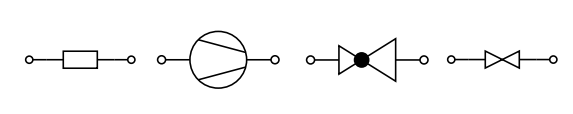
\includegraphics[scale = 0.5]{img_other/non_pipe_elements.png}
    \end{figure}
    \item No refinement per pipe (grid creator)
    \begin{center}    % Graphic for TeX using PGF
% Title: /home/karol/Documents/UNIVERSITA/POLITO/PRESENTATIONS/SHIMMER_2024_01/img_code/pipe_network_ref.dia
% Creator: Dia v0.97.3
% CreationDate: Tue Jan 30 23:44:31 2024
% For: karol
% \usepackage{tikz}
% The following commands are not supported in PSTricks at present
% We define them conditionally, so when they are implemented,
% this pgf file will use them.
\ifx\du\undefined
  \newlength{\du}
\fi
\setlength{\du}{8\unitlength}
\begin{tikzpicture}[even odd rule]
\pgftransformxscale{1.000000}
\pgftransformyscale{-1.000000}
\definecolor{dialinecolor}{rgb}{0.000000, 0.000000, 0.000000}
\pgfsetstrokecolor{dialinecolor}
\pgfsetstrokeopacity{1.000000}
\definecolor{diafillcolor}{rgb}{1.000000, 1.000000, 1.000000}
\pgfsetfillcolor{diafillcolor}
\pgfsetfillopacity{1.000000}
\pgfsetlinewidth{0.100000\du}
\pgfsetdash{}{0pt}
\pgfsetmiterjoin
\definecolor{diafillcolor}{rgb}{1.000000, 1.000000, 1.000000}
\pgfsetfillcolor{diafillcolor}
\pgfsetfillopacity{1.000000}
\pgfpathellipse{\pgfpoint{39.693572\du}{5.676288\du}}{\pgfpoint{0.693572\du}{0\du}}{\pgfpoint{0\du}{0.676288\du}}
\pgfusepath{fill}
\definecolor{dialinecolor}{rgb}{0.937255, 0.000000, 0.701961}
\pgfsetstrokecolor{dialinecolor}
\pgfsetstrokeopacity{1.000000}
\pgfpathellipse{\pgfpoint{39.693572\du}{5.676288\du}}{\pgfpoint{0.693572\du}{0\du}}{\pgfpoint{0\du}{0.676288\du}}
\pgfusepath{stroke}
% setfont left to latex
% setfont left to latex
\definecolor{dialinecolor}{rgb}{0.000000, 0.000000, 0.000000}
\pgfsetstrokecolor{dialinecolor}
\pgfsetstrokeopacity{1.000000}
\definecolor{diafillcolor}{rgb}{0.000000, 0.000000, 0.000000}
\pgfsetfillcolor{diafillcolor}
\pgfsetfillopacity{1.000000}
\node[anchor=base,inner sep=0pt, outer sep=0pt,color=dialinecolor] at (39.693572\du,5.961288\du){};
\pgfsetlinewidth{0.100000\du}
\pgfsetdash{}{0pt}
\pgfsetmiterjoin
\definecolor{diafillcolor}{rgb}{1.000000, 1.000000, 1.000000}
\pgfsetfillcolor{diafillcolor}
\pgfsetfillopacity{1.000000}
\pgfpathellipse{\pgfpoint{39.693572\du}{9.676288\du}}{\pgfpoint{0.693572\du}{0\du}}{\pgfpoint{0\du}{0.676288\du}}
\pgfusepath{fill}
\definecolor{dialinecolor}{rgb}{0.937255, 0.000000, 0.701961}
\pgfsetstrokecolor{dialinecolor}
\pgfsetstrokeopacity{1.000000}
\pgfpathellipse{\pgfpoint{39.693572\du}{9.676288\du}}{\pgfpoint{0.693572\du}{0\du}}{\pgfpoint{0\du}{0.676288\du}}
\pgfusepath{stroke}
% setfont left to latex
% setfont left to latex
\definecolor{dialinecolor}{rgb}{0.000000, 0.000000, 0.000000}
\pgfsetstrokecolor{dialinecolor}
\pgfsetstrokeopacity{1.000000}
\definecolor{diafillcolor}{rgb}{0.000000, 0.000000, 0.000000}
\pgfsetfillcolor{diafillcolor}
\pgfsetfillopacity{1.000000}
\node[anchor=base,inner sep=0pt, outer sep=0pt,color=dialinecolor] at (39.693572\du,9.961288\du){};
\pgfsetlinewidth{0.100000\du}
\pgfsetdash{}{0pt}
\pgfsetmiterjoin
\definecolor{diafillcolor}{rgb}{1.000000, 1.000000, 1.000000}
\pgfsetfillcolor{diafillcolor}
\pgfsetfillopacity{1.000000}
\pgfpathellipse{\pgfpoint{37.753572\du}{13.676288\du}}{\pgfpoint{0.753572\du}{0\du}}{\pgfpoint{0\du}{0.676288\du}}
\pgfusepath{fill}
\definecolor{dialinecolor}{rgb}{0.937255, 0.000000, 0.701961}
\pgfsetstrokecolor{dialinecolor}
\pgfsetstrokeopacity{1.000000}
\pgfpathellipse{\pgfpoint{37.753572\du}{13.676288\du}}{\pgfpoint{0.753572\du}{0\du}}{\pgfpoint{0\du}{0.676288\du}}
\pgfusepath{stroke}
% setfont left to latex
% setfont left to latex
\definecolor{dialinecolor}{rgb}{0.000000, 0.000000, 0.000000}
\pgfsetstrokecolor{dialinecolor}
\pgfsetstrokeopacity{1.000000}
\definecolor{diafillcolor}{rgb}{0.000000, 0.000000, 0.000000}
\pgfsetfillcolor{diafillcolor}
\pgfsetfillopacity{1.000000}
\node[anchor=base,inner sep=0pt, outer sep=0pt,color=dialinecolor] at (37.753572\du,13.961288\du){};
\pgfsetlinewidth{0.100000\du}
\pgfsetdash{}{0pt}
\pgfsetmiterjoin
\definecolor{diafillcolor}{rgb}{1.000000, 1.000000, 1.000000}
\pgfsetfillcolor{diafillcolor}
\pgfsetfillopacity{1.000000}
\pgfpathellipse{\pgfpoint{45.693572\du}{13.676288\du}}{\pgfpoint{0.693572\du}{0\du}}{\pgfpoint{0\du}{0.676288\du}}
\pgfusepath{fill}
\definecolor{dialinecolor}{rgb}{0.937255, 0.000000, 0.701961}
\pgfsetstrokecolor{dialinecolor}
\pgfsetstrokeopacity{1.000000}
\pgfpathellipse{\pgfpoint{45.693572\du}{13.676288\du}}{\pgfpoint{0.693572\du}{0\du}}{\pgfpoint{0\du}{0.676288\du}}
\pgfusepath{stroke}
% setfont left to latex
% setfont left to latex
\definecolor{dialinecolor}{rgb}{0.000000, 0.000000, 0.000000}
\pgfsetstrokecolor{dialinecolor}
\pgfsetstrokeopacity{1.000000}
\definecolor{diafillcolor}{rgb}{0.000000, 0.000000, 0.000000}
\pgfsetfillcolor{diafillcolor}
\pgfsetfillopacity{1.000000}
\node[anchor=base,inner sep=0pt, outer sep=0pt,color=dialinecolor] at (45.693572\du,13.961288\du){};
\pgfsetlinewidth{0.100000\du}
\pgfsetdash{}{0pt}
\pgfsetmiterjoin
\definecolor{diafillcolor}{rgb}{1.000000, 1.000000, 1.000000}
\pgfsetfillcolor{diafillcolor}
\pgfsetfillopacity{1.000000}
\pgfpathellipse{\pgfpoint{41.693572\du}{13.676288\du}}{\pgfpoint{0.693572\du}{0\du}}{\pgfpoint{0\du}{0.676288\du}}
\pgfusepath{fill}
\definecolor{dialinecolor}{rgb}{0.937255, 0.000000, 0.701961}
\pgfsetstrokecolor{dialinecolor}
\pgfsetstrokeopacity{1.000000}
\pgfpathellipse{\pgfpoint{41.693572\du}{13.676288\du}}{\pgfpoint{0.693572\du}{0\du}}{\pgfpoint{0\du}{0.676288\du}}
\pgfusepath{stroke}
% setfont left to latex
% setfont left to latex
\definecolor{dialinecolor}{rgb}{0.000000, 0.000000, 0.000000}
\pgfsetstrokecolor{dialinecolor}
\pgfsetstrokeopacity{1.000000}
\definecolor{diafillcolor}{rgb}{0.000000, 0.000000, 0.000000}
\pgfsetfillcolor{diafillcolor}
\pgfsetfillopacity{1.000000}
\node[anchor=base,inner sep=0pt, outer sep=0pt,color=dialinecolor] at (41.693572\du,13.961288\du){};
\pgfsetlinewidth{0.050000\du}
\pgfsetdash{}{0pt}
\pgfsetbuttcap
{
\definecolor{diafillcolor}{rgb}{0.000000, 0.501961, 0.501961}
\pgfsetfillcolor{diafillcolor}
\pgfsetfillopacity{1.000000}
% was here!!!
\definecolor{dialinecolor}{rgb}{0.000000, 0.501961, 0.501961}
\pgfsetstrokecolor{dialinecolor}
\pgfsetstrokeopacity{1.000000}
\draw (39.693572\du,6.351417\du)--(39.693570\du,9.000000\du);
}
\pgfsetlinewidth{0.050000\du}
\pgfsetdash{}{0pt}
\pgfsetbuttcap
{
\definecolor{diafillcolor}{rgb}{0.000000, 0.501961, 0.501961}
\pgfsetfillcolor{diafillcolor}
\pgfsetfillopacity{1.000000}
% was here!!!
\definecolor{dialinecolor}{rgb}{0.000000, 0.501961, 0.501961}
\pgfsetstrokecolor{dialinecolor}
\pgfsetstrokeopacity{1.000000}
\draw (39.693570\du,10.352600\du)--(37.753570\du,13.000000\du);
}
\pgfsetlinewidth{0.050000\du}
\pgfsetdash{}{0pt}
\pgfsetbuttcap
{
\definecolor{diafillcolor}{rgb}{0.000000, 0.501961, 0.501961}
\pgfsetfillcolor{diafillcolor}
\pgfsetfillopacity{1.000000}
% was here!!!
\definecolor{dialinecolor}{rgb}{0.000000, 0.501961, 0.501961}
\pgfsetstrokecolor{dialinecolor}
\pgfsetstrokeopacity{1.000000}
\draw (39.693570\du,10.352600\du)--(41.693600\du,13.000000\du);
}
\pgfsetlinewidth{0.050000\du}
\pgfsetdash{}{0pt}
\pgfsetbuttcap
{
\definecolor{diafillcolor}{rgb}{0.000000, 0.501961, 0.501961}
\pgfsetfillcolor{diafillcolor}
\pgfsetfillopacity{1.000000}
% was here!!!
\definecolor{dialinecolor}{rgb}{0.000000, 0.501961, 0.501961}
\pgfsetstrokecolor{dialinecolor}
\pgfsetstrokeopacity{1.000000}
\draw (41.000000\du,13.676300\du)--(38.507140\du,13.676300\du);
}
\pgfsetlinewidth{0.050000\du}
\pgfsetdash{}{0pt}
\pgfsetbuttcap
{
\definecolor{diafillcolor}{rgb}{0.000000, 0.501961, 0.501961}
\pgfsetfillcolor{diafillcolor}
\pgfsetfillopacity{1.000000}
% was here!!!
\definecolor{dialinecolor}{rgb}{0.000000, 0.501961, 0.501961}
\pgfsetstrokecolor{dialinecolor}
\pgfsetstrokeopacity{1.000000}
\draw (42.387100\du,13.676300\du)--(45.000000\du,13.676300\du);
}
% setfont left to latex
% setfont left to latex
\definecolor{dialinecolor}{rgb}{0.000000, 0.501961, 0.501961}
\pgfsetstrokecolor{dialinecolor}
\pgfsetstrokeopacity{1.000000}
\definecolor{diafillcolor}{rgb}{0.000000, 0.501961, 0.501961}
\pgfsetfillcolor{diafillcolor}
\pgfsetfillopacity{1.000000}
\node[anchor=base west,inner sep=0pt,outer sep=0pt,color=dialinecolor] at (39.000000\du,8.000000\du){};
% setfont left to latex
% setfont left to latex
\definecolor{dialinecolor}{rgb}{0.000000, 0.501961, 0.501961}
\pgfsetstrokecolor{dialinecolor}
\pgfsetstrokeopacity{1.000000}
\definecolor{diafillcolor}{rgb}{0.000000, 0.501961, 0.501961}
\pgfsetfillcolor{diafillcolor}
\pgfsetfillopacity{1.000000}
\node[anchor=base west,inner sep=0pt,outer sep=0pt,color=dialinecolor] at (38.000000\du,12.000000\du){};
% setfont left to latex
% setfont left to latex
\definecolor{dialinecolor}{rgb}{0.000000, 0.501961, 0.501961}
\pgfsetstrokecolor{dialinecolor}
\pgfsetstrokeopacity{1.000000}
\definecolor{diafillcolor}{rgb}{0.000000, 0.501961, 0.501961}
\pgfsetfillcolor{diafillcolor}
\pgfsetfillopacity{1.000000}
\node[anchor=base west,inner sep=0pt,outer sep=0pt,color=dialinecolor] at (42.000000\du,12.000000\du){};
% setfont left to latex
% setfont left to latex
\definecolor{dialinecolor}{rgb}{0.000000, 0.501961, 0.501961}
\pgfsetstrokecolor{dialinecolor}
\pgfsetstrokeopacity{1.000000}
\definecolor{diafillcolor}{rgb}{0.000000, 0.501961, 0.501961}
\pgfsetfillcolor{diafillcolor}
\pgfsetfillopacity{1.000000}
\node[anchor=base west,inner sep=0pt,outer sep=0pt,color=dialinecolor] at (39.450000\du,14.900000\du){};
% setfont left to latex
% setfont left to latex
\definecolor{dialinecolor}{rgb}{0.000000, 0.501961, 0.501961}
\pgfsetstrokecolor{dialinecolor}
\pgfsetstrokeopacity{1.000000}
\definecolor{diafillcolor}{rgb}{0.000000, 0.501961, 0.501961}
\pgfsetfillcolor{diafillcolor}
\pgfsetfillopacity{1.000000}
\node[anchor=base west,inner sep=0pt,outer sep=0pt,color=dialinecolor] at (43.590000\du,14.895000\du){};
\pgfsetlinewidth{0.100000\du}
\pgfsetdash{}{0pt}
\definecolor{diafillcolor}{rgb}{1.000000, 1.000000, 1.000000}
\pgfsetfillcolor{diafillcolor}
\pgfsetfillopacity{1.000000}
\pgfpathellipse{\pgfpoint{39.700000\du}{7.499999\du}}{\pgfpoint{0.093210\du}{0\du}}{\pgfpoint{0\du}{0.076999\du}}
\pgfusepath{fill}
\definecolor{dialinecolor}{rgb}{0.501961, 0.000000, 0.501961}
\pgfsetstrokecolor{dialinecolor}
\pgfsetstrokeopacity{1.000000}
\pgfpathellipse{\pgfpoint{39.700000\du}{7.499999\du}}{\pgfpoint{0.093210\du}{0\du}}{\pgfpoint{0\du}{0.076999\du}}
\pgfusepath{stroke}
\pgfsetlinewidth{0.100000\du}
\pgfsetdash{}{0pt}
\definecolor{diafillcolor}{rgb}{1.000000, 1.000000, 1.000000}
\pgfsetfillcolor{diafillcolor}
\pgfsetfillopacity{1.000000}
\pgfpathellipse{\pgfpoint{39.700000\du}{6.999999\du}}{\pgfpoint{0.093210\du}{0\du}}{\pgfpoint{0\du}{0.076999\du}}
\pgfusepath{fill}
\definecolor{dialinecolor}{rgb}{0.501961, 0.000000, 0.501961}
\pgfsetstrokecolor{dialinecolor}
\pgfsetstrokeopacity{1.000000}
\pgfpathellipse{\pgfpoint{39.700000\du}{6.999999\du}}{\pgfpoint{0.093210\du}{0\du}}{\pgfpoint{0\du}{0.076999\du}}
\pgfusepath{stroke}
\pgfsetlinewidth{0.100000\du}
\pgfsetdash{}{0pt}
\definecolor{diafillcolor}{rgb}{1.000000, 1.000000, 1.000000}
\pgfsetfillcolor{diafillcolor}
\pgfsetfillopacity{1.000000}
\pgfpathellipse{\pgfpoint{39.700000\du}{7.999999\du}}{\pgfpoint{0.093210\du}{0\du}}{\pgfpoint{0\du}{0.076999\du}}
\pgfusepath{fill}
\definecolor{dialinecolor}{rgb}{0.501961, 0.000000, 0.501961}
\pgfsetstrokecolor{dialinecolor}
\pgfsetstrokeopacity{1.000000}
\pgfpathellipse{\pgfpoint{39.700000\du}{7.999999\du}}{\pgfpoint{0.093210\du}{0\du}}{\pgfpoint{0\du}{0.076999\du}}
\pgfusepath{stroke}
\pgfsetlinewidth{0.100000\du}
\pgfsetdash{}{0pt}
\definecolor{diafillcolor}{rgb}{1.000000, 1.000000, 1.000000}
\pgfsetfillcolor{diafillcolor}
\pgfsetfillopacity{1.000000}
\pgfpathellipse{\pgfpoint{39.700000\du}{8.499999\du}}{\pgfpoint{0.093210\du}{0\du}}{\pgfpoint{0\du}{0.076999\du}}
\pgfusepath{fill}
\definecolor{dialinecolor}{rgb}{0.501961, 0.000000, 0.501961}
\pgfsetstrokecolor{dialinecolor}
\pgfsetstrokeopacity{1.000000}
\pgfpathellipse{\pgfpoint{39.700000\du}{8.499999\du}}{\pgfpoint{0.093210\du}{0\du}}{\pgfpoint{0\du}{0.076999\du}}
\pgfusepath{stroke}
\pgfsetlinewidth{0.100000\du}
\pgfsetdash{}{0pt}
\definecolor{diafillcolor}{rgb}{1.000000, 1.000000, 1.000000}
\pgfsetfillcolor{diafillcolor}
\pgfsetfillopacity{1.000000}
\pgfpathellipse{\pgfpoint{40.500000\du}{11.499999\du}}{\pgfpoint{0.093210\du}{0\du}}{\pgfpoint{0\du}{0.076999\du}}
\pgfusepath{fill}
\definecolor{dialinecolor}{rgb}{0.501961, 0.000000, 0.501961}
\pgfsetstrokecolor{dialinecolor}
\pgfsetstrokeopacity{1.000000}
\pgfpathellipse{\pgfpoint{40.500000\du}{11.499999\du}}{\pgfpoint{0.093210\du}{0\du}}{\pgfpoint{0\du}{0.076999\du}}
\pgfusepath{stroke}
\pgfsetlinewidth{0.100000\du}
\pgfsetdash{}{0pt}
\definecolor{diafillcolor}{rgb}{1.000000, 1.000000, 1.000000}
\pgfsetfillcolor{diafillcolor}
\pgfsetfillopacity{1.000000}
\pgfpathellipse{\pgfpoint{40.193210\du}{10.976999\du}}{\pgfpoint{0.093210\du}{0\du}}{\pgfpoint{0\du}{0.076999\du}}
\pgfusepath{fill}
\definecolor{dialinecolor}{rgb}{0.501961, 0.000000, 0.501961}
\pgfsetstrokecolor{dialinecolor}
\pgfsetstrokeopacity{1.000000}
\pgfpathellipse{\pgfpoint{40.193210\du}{10.976999\du}}{\pgfpoint{0.093210\du}{0\du}}{\pgfpoint{0\du}{0.076999\du}}
\pgfusepath{stroke}
\pgfsetlinewidth{0.100000\du}
\pgfsetdash{}{0pt}
\definecolor{diafillcolor}{rgb}{1.000000, 1.000000, 1.000000}
\pgfsetfillcolor{diafillcolor}
\pgfsetfillopacity{1.000000}
\pgfpathellipse{\pgfpoint{40.900000\du}{11.999999\du}}{\pgfpoint{0.093210\du}{0\du}}{\pgfpoint{0\du}{0.076999\du}}
\pgfusepath{fill}
\definecolor{dialinecolor}{rgb}{0.501961, 0.000000, 0.501961}
\pgfsetstrokecolor{dialinecolor}
\pgfsetstrokeopacity{1.000000}
\pgfpathellipse{\pgfpoint{40.900000\du}{11.999999\du}}{\pgfpoint{0.093210\du}{0\du}}{\pgfpoint{0\du}{0.076999\du}}
\pgfusepath{stroke}
\pgfsetlinewidth{0.100000\du}
\pgfsetdash{}{0pt}
\definecolor{diafillcolor}{rgb}{1.000000, 1.000000, 1.000000}
\pgfsetfillcolor{diafillcolor}
\pgfsetfillopacity{1.000000}
\pgfpathellipse{\pgfpoint{41.300010\du}{12.499999\du}}{\pgfpoint{0.093210\du}{0\du}}{\pgfpoint{0\du}{0.076999\du}}
\pgfusepath{fill}
\definecolor{dialinecolor}{rgb}{0.501961, 0.000000, 0.501961}
\pgfsetstrokecolor{dialinecolor}
\pgfsetstrokeopacity{1.000000}
\pgfpathellipse{\pgfpoint{41.300010\du}{12.499999\du}}{\pgfpoint{0.093210\du}{0\du}}{\pgfpoint{0\du}{0.076999\du}}
\pgfusepath{stroke}
\pgfsetlinewidth{0.100000\du}
\pgfsetdash{}{0pt}
\definecolor{diafillcolor}{rgb}{1.000000, 1.000000, 1.000000}
\pgfsetfillcolor{diafillcolor}
\pgfsetfillopacity{1.000000}
\pgfpathellipse{\pgfpoint{38.800000\du}{11.499999\du}}{\pgfpoint{0.093210\du}{0\du}}{\pgfpoint{0\du}{0.076999\du}}
\pgfusepath{fill}
\definecolor{dialinecolor}{rgb}{0.501961, 0.000000, 0.501961}
\pgfsetstrokecolor{dialinecolor}
\pgfsetstrokeopacity{1.000000}
\pgfpathellipse{\pgfpoint{38.800000\du}{11.499999\du}}{\pgfpoint{0.093210\du}{0\du}}{\pgfpoint{0\du}{0.076999\du}}
\pgfusepath{stroke}
\pgfsetlinewidth{0.100000\du}
\pgfsetdash{}{0pt}
\definecolor{diafillcolor}{rgb}{1.000000, 1.000000, 1.000000}
\pgfsetfillcolor{diafillcolor}
\pgfsetfillopacity{1.000000}
\pgfpathellipse{\pgfpoint{39.193210\du}{10.976999\du}}{\pgfpoint{0.093210\du}{0\du}}{\pgfpoint{0\du}{0.076999\du}}
\pgfusepath{fill}
\definecolor{dialinecolor}{rgb}{0.501961, 0.000000, 0.501961}
\pgfsetstrokecolor{dialinecolor}
\pgfsetstrokeopacity{1.000000}
\pgfpathellipse{\pgfpoint{39.193210\du}{10.976999\du}}{\pgfpoint{0.093210\du}{0\du}}{\pgfpoint{0\du}{0.076999\du}}
\pgfusepath{stroke}
\pgfsetlinewidth{0.100000\du}
\pgfsetdash{}{0pt}
\definecolor{diafillcolor}{rgb}{1.000000, 1.000000, 1.000000}
\pgfsetfillcolor{diafillcolor}
\pgfsetfillopacity{1.000000}
\pgfpathellipse{\pgfpoint{38.500000\du}{11.999999\du}}{\pgfpoint{0.093210\du}{0\du}}{\pgfpoint{0\du}{0.076999\du}}
\pgfusepath{fill}
\definecolor{dialinecolor}{rgb}{0.501961, 0.000000, 0.501961}
\pgfsetstrokecolor{dialinecolor}
\pgfsetstrokeopacity{1.000000}
\pgfpathellipse{\pgfpoint{38.500000\du}{11.999999\du}}{\pgfpoint{0.093210\du}{0\du}}{\pgfpoint{0\du}{0.076999\du}}
\pgfusepath{stroke}
\pgfsetlinewidth{0.100000\du}
\pgfsetdash{}{0pt}
\definecolor{diafillcolor}{rgb}{1.000000, 1.000000, 1.000000}
\pgfsetfillcolor{diafillcolor}
\pgfsetfillopacity{1.000000}
\pgfpathellipse{\pgfpoint{38.100000\du}{12.499999\du}}{\pgfpoint{0.093210\du}{0\du}}{\pgfpoint{0\du}{0.076999\du}}
\pgfusepath{fill}
\definecolor{dialinecolor}{rgb}{0.501961, 0.000000, 0.501961}
\pgfsetstrokecolor{dialinecolor}
\pgfsetstrokeopacity{1.000000}
\pgfpathellipse{\pgfpoint{38.100000\du}{12.499999\du}}{\pgfpoint{0.093210\du}{0\du}}{\pgfpoint{0\du}{0.076999\du}}
\pgfusepath{stroke}
\pgfsetlinewidth{0.100000\du}
\pgfsetdash{}{0pt}
\definecolor{diafillcolor}{rgb}{1.000000, 1.000000, 1.000000}
\pgfsetfillcolor{diafillcolor}
\pgfsetfillopacity{1.000000}
\pgfpathellipse{\pgfpoint{39.500000\du}{13.699999\du}}{\pgfpoint{0.093210\du}{0\du}}{\pgfpoint{0\du}{0.076999\du}}
\pgfusepath{fill}
\definecolor{dialinecolor}{rgb}{0.501961, 0.000000, 0.501961}
\pgfsetstrokecolor{dialinecolor}
\pgfsetstrokeopacity{1.000000}
\pgfpathellipse{\pgfpoint{39.500000\du}{13.699999\du}}{\pgfpoint{0.093210\du}{0\du}}{\pgfpoint{0\du}{0.076999\du}}
\pgfusepath{stroke}
\pgfsetlinewidth{0.100000\du}
\pgfsetdash{}{0pt}
\definecolor{diafillcolor}{rgb}{1.000000, 1.000000, 1.000000}
\pgfsetfillcolor{diafillcolor}
\pgfsetfillopacity{1.000000}
\pgfpathellipse{\pgfpoint{39.000000\du}{13.699999\du}}{\pgfpoint{0.093210\du}{0\du}}{\pgfpoint{0\du}{0.076999\du}}
\pgfusepath{fill}
\definecolor{dialinecolor}{rgb}{0.501961, 0.000000, 0.501961}
\pgfsetstrokecolor{dialinecolor}
\pgfsetstrokeopacity{1.000000}
\pgfpathellipse{\pgfpoint{39.000000\du}{13.699999\du}}{\pgfpoint{0.093210\du}{0\du}}{\pgfpoint{0\du}{0.076999\du}}
\pgfusepath{stroke}
\pgfsetlinewidth{0.100000\du}
\pgfsetdash{}{0pt}
\definecolor{diafillcolor}{rgb}{1.000000, 1.000000, 1.000000}
\pgfsetfillcolor{diafillcolor}
\pgfsetfillopacity{1.000000}
\pgfpathellipse{\pgfpoint{40.000000\du}{13.699999\du}}{\pgfpoint{0.093210\du}{0\du}}{\pgfpoint{0\du}{0.076999\du}}
\pgfusepath{fill}
\definecolor{dialinecolor}{rgb}{0.501961, 0.000000, 0.501961}
\pgfsetstrokecolor{dialinecolor}
\pgfsetstrokeopacity{1.000000}
\pgfpathellipse{\pgfpoint{40.000000\du}{13.699999\du}}{\pgfpoint{0.093210\du}{0\du}}{\pgfpoint{0\du}{0.076999\du}}
\pgfusepath{stroke}
\pgfsetlinewidth{0.100000\du}
\pgfsetdash{}{0pt}
\definecolor{diafillcolor}{rgb}{1.000000, 1.000000, 1.000000}
\pgfsetfillcolor{diafillcolor}
\pgfsetfillopacity{1.000000}
\pgfpathellipse{\pgfpoint{40.500000\du}{13.699999\du}}{\pgfpoint{0.093210\du}{0\du}}{\pgfpoint{0\du}{0.076999\du}}
\pgfusepath{fill}
\definecolor{dialinecolor}{rgb}{0.501961, 0.000000, 0.501961}
\pgfsetstrokecolor{dialinecolor}
\pgfsetstrokeopacity{1.000000}
\pgfpathellipse{\pgfpoint{40.500000\du}{13.699999\du}}{\pgfpoint{0.093210\du}{0\du}}{\pgfpoint{0\du}{0.076999\du}}
\pgfusepath{stroke}
\pgfsetlinewidth{0.100000\du}
\pgfsetdash{}{0pt}
\definecolor{diafillcolor}{rgb}{1.000000, 1.000000, 1.000000}
\pgfsetfillcolor{diafillcolor}
\pgfsetfillopacity{1.000000}
\pgfpathellipse{\pgfpoint{43.493210\du}{13.676999\du}}{\pgfpoint{0.093210\du}{0\du}}{\pgfpoint{0\du}{0.076999\du}}
\pgfusepath{fill}
\definecolor{dialinecolor}{rgb}{0.501961, 0.000000, 0.501961}
\pgfsetstrokecolor{dialinecolor}
\pgfsetstrokeopacity{1.000000}
\pgfpathellipse{\pgfpoint{43.493210\du}{13.676999\du}}{\pgfpoint{0.093210\du}{0\du}}{\pgfpoint{0\du}{0.076999\du}}
\pgfusepath{stroke}
\pgfsetlinewidth{0.100000\du}
\pgfsetdash{}{0pt}
\definecolor{diafillcolor}{rgb}{1.000000, 1.000000, 1.000000}
\pgfsetfillcolor{diafillcolor}
\pgfsetfillopacity{1.000000}
\pgfpathellipse{\pgfpoint{42.993210\du}{13.676999\du}}{\pgfpoint{0.093210\du}{0\du}}{\pgfpoint{0\du}{0.076999\du}}
\pgfusepath{fill}
\definecolor{dialinecolor}{rgb}{0.501961, 0.000000, 0.501961}
\pgfsetstrokecolor{dialinecolor}
\pgfsetstrokeopacity{1.000000}
\pgfpathellipse{\pgfpoint{42.993210\du}{13.676999\du}}{\pgfpoint{0.093210\du}{0\du}}{\pgfpoint{0\du}{0.076999\du}}
\pgfusepath{stroke}
\pgfsetlinewidth{0.100000\du}
\pgfsetdash{}{0pt}
\definecolor{diafillcolor}{rgb}{1.000000, 1.000000, 1.000000}
\pgfsetfillcolor{diafillcolor}
\pgfsetfillopacity{1.000000}
\pgfpathellipse{\pgfpoint{43.993210\du}{13.676999\du}}{\pgfpoint{0.093210\du}{0\du}}{\pgfpoint{0\du}{0.076999\du}}
\pgfusepath{fill}
\definecolor{dialinecolor}{rgb}{0.501961, 0.000000, 0.501961}
\pgfsetstrokecolor{dialinecolor}
\pgfsetstrokeopacity{1.000000}
\pgfpathellipse{\pgfpoint{43.993210\du}{13.676999\du}}{\pgfpoint{0.093210\du}{0\du}}{\pgfpoint{0\du}{0.076999\du}}
\pgfusepath{stroke}
\pgfsetlinewidth{0.100000\du}
\pgfsetdash{}{0pt}
\definecolor{diafillcolor}{rgb}{1.000000, 1.000000, 1.000000}
\pgfsetfillcolor{diafillcolor}
\pgfsetfillopacity{1.000000}
\pgfpathellipse{\pgfpoint{44.493210\du}{13.676999\du}}{\pgfpoint{0.093210\du}{0\du}}{\pgfpoint{0\du}{0.076999\du}}
\pgfusepath{fill}
\definecolor{dialinecolor}{rgb}{0.501961, 0.000000, 0.501961}
\pgfsetstrokecolor{dialinecolor}
\pgfsetstrokeopacity{1.000000}
\pgfpathellipse{\pgfpoint{44.493210\du}{13.676999\du}}{\pgfpoint{0.093210\du}{0\du}}{\pgfpoint{0\du}{0.076999\du}}
\pgfusepath{stroke}
\pgfsetlinewidth{0.100000\du}
\pgfsetdash{}{0pt}
\pgfsetmiterjoin
\definecolor{diafillcolor}{rgb}{1.000000, 1.000000, 1.000000}
\pgfsetfillcolor{diafillcolor}
\pgfsetfillopacity{1.000000}
\pgfpathellipse{\pgfpoint{24.693572\du}{5.676288\du}}{\pgfpoint{0.693572\du}{0\du}}{\pgfpoint{0\du}{0.676288\du}}
\pgfusepath{fill}
\definecolor{dialinecolor}{rgb}{0.937255, 0.000000, 0.701961}
\pgfsetstrokecolor{dialinecolor}
\pgfsetstrokeopacity{1.000000}
\pgfpathellipse{\pgfpoint{24.693572\du}{5.676288\du}}{\pgfpoint{0.693572\du}{0\du}}{\pgfpoint{0\du}{0.676288\du}}
\pgfusepath{stroke}
% setfont left to latex
% setfont left to latex
\definecolor{dialinecolor}{rgb}{0.000000, 0.000000, 0.000000}
\pgfsetstrokecolor{dialinecolor}
\pgfsetstrokeopacity{1.000000}
\definecolor{diafillcolor}{rgb}{0.000000, 0.000000, 0.000000}
\pgfsetfillcolor{diafillcolor}
\pgfsetfillopacity{1.000000}
\node[anchor=base,inner sep=0pt, outer sep=0pt,color=dialinecolor] at (24.693572\du,5.961288\du){};
\pgfsetlinewidth{0.100000\du}
\pgfsetdash{}{0pt}
\pgfsetmiterjoin
\definecolor{diafillcolor}{rgb}{1.000000, 1.000000, 1.000000}
\pgfsetfillcolor{diafillcolor}
\pgfsetfillopacity{1.000000}
\pgfpathellipse{\pgfpoint{24.693572\du}{9.676288\du}}{\pgfpoint{0.693572\du}{0\du}}{\pgfpoint{0\du}{0.676288\du}}
\pgfusepath{fill}
\definecolor{dialinecolor}{rgb}{0.937255, 0.000000, 0.701961}
\pgfsetstrokecolor{dialinecolor}
\pgfsetstrokeopacity{1.000000}
\pgfpathellipse{\pgfpoint{24.693572\du}{9.676288\du}}{\pgfpoint{0.693572\du}{0\du}}{\pgfpoint{0\du}{0.676288\du}}
\pgfusepath{stroke}
% setfont left to latex
% setfont left to latex
\definecolor{dialinecolor}{rgb}{0.000000, 0.000000, 0.000000}
\pgfsetstrokecolor{dialinecolor}
\pgfsetstrokeopacity{1.000000}
\definecolor{diafillcolor}{rgb}{0.000000, 0.000000, 0.000000}
\pgfsetfillcolor{diafillcolor}
\pgfsetfillopacity{1.000000}
\node[anchor=base,inner sep=0pt, outer sep=0pt,color=dialinecolor] at (24.693572\du,9.961288\du){};
\pgfsetlinewidth{0.100000\du}
\pgfsetdash{}{0pt}
\pgfsetmiterjoin
\definecolor{diafillcolor}{rgb}{1.000000, 1.000000, 1.000000}
\pgfsetfillcolor{diafillcolor}
\pgfsetfillopacity{1.000000}
\pgfpathellipse{\pgfpoint{22.753572\du}{13.676288\du}}{\pgfpoint{0.753572\du}{0\du}}{\pgfpoint{0\du}{0.676288\du}}
\pgfusepath{fill}
\definecolor{dialinecolor}{rgb}{0.937255, 0.000000, 0.701961}
\pgfsetstrokecolor{dialinecolor}
\pgfsetstrokeopacity{1.000000}
\pgfpathellipse{\pgfpoint{22.753572\du}{13.676288\du}}{\pgfpoint{0.753572\du}{0\du}}{\pgfpoint{0\du}{0.676288\du}}
\pgfusepath{stroke}
% setfont left to latex
% setfont left to latex
\definecolor{dialinecolor}{rgb}{0.000000, 0.000000, 0.000000}
\pgfsetstrokecolor{dialinecolor}
\pgfsetstrokeopacity{1.000000}
\definecolor{diafillcolor}{rgb}{0.000000, 0.000000, 0.000000}
\pgfsetfillcolor{diafillcolor}
\pgfsetfillopacity{1.000000}
\node[anchor=base,inner sep=0pt, outer sep=0pt,color=dialinecolor] at (22.753572\du,13.961288\du){};
\pgfsetlinewidth{0.100000\du}
\pgfsetdash{}{0pt}
\pgfsetmiterjoin
\definecolor{diafillcolor}{rgb}{1.000000, 1.000000, 1.000000}
\pgfsetfillcolor{diafillcolor}
\pgfsetfillopacity{1.000000}
\pgfpathellipse{\pgfpoint{30.693572\du}{13.676288\du}}{\pgfpoint{0.693572\du}{0\du}}{\pgfpoint{0\du}{0.676288\du}}
\pgfusepath{fill}
\definecolor{dialinecolor}{rgb}{0.937255, 0.000000, 0.701961}
\pgfsetstrokecolor{dialinecolor}
\pgfsetstrokeopacity{1.000000}
\pgfpathellipse{\pgfpoint{30.693572\du}{13.676288\du}}{\pgfpoint{0.693572\du}{0\du}}{\pgfpoint{0\du}{0.676288\du}}
\pgfusepath{stroke}
% setfont left to latex
% setfont left to latex
\definecolor{dialinecolor}{rgb}{0.000000, 0.000000, 0.000000}
\pgfsetstrokecolor{dialinecolor}
\pgfsetstrokeopacity{1.000000}
\definecolor{diafillcolor}{rgb}{0.000000, 0.000000, 0.000000}
\pgfsetfillcolor{diafillcolor}
\pgfsetfillopacity{1.000000}
\node[anchor=base,inner sep=0pt, outer sep=0pt,color=dialinecolor] at (30.693572\du,13.961288\du){};
\pgfsetlinewidth{0.100000\du}
\pgfsetdash{}{0pt}
\pgfsetmiterjoin
\definecolor{diafillcolor}{rgb}{1.000000, 1.000000, 1.000000}
\pgfsetfillcolor{diafillcolor}
\pgfsetfillopacity{1.000000}
\pgfpathellipse{\pgfpoint{26.693572\du}{13.676288\du}}{\pgfpoint{0.693572\du}{0\du}}{\pgfpoint{0\du}{0.676288\du}}
\pgfusepath{fill}
\definecolor{dialinecolor}{rgb}{0.937255, 0.000000, 0.701961}
\pgfsetstrokecolor{dialinecolor}
\pgfsetstrokeopacity{1.000000}
\pgfpathellipse{\pgfpoint{26.693572\du}{13.676288\du}}{\pgfpoint{0.693572\du}{0\du}}{\pgfpoint{0\du}{0.676288\du}}
\pgfusepath{stroke}
% setfont left to latex
% setfont left to latex
\definecolor{dialinecolor}{rgb}{0.000000, 0.000000, 0.000000}
\pgfsetstrokecolor{dialinecolor}
\pgfsetstrokeopacity{1.000000}
\definecolor{diafillcolor}{rgb}{0.000000, 0.000000, 0.000000}
\pgfsetfillcolor{diafillcolor}
\pgfsetfillopacity{1.000000}
\node[anchor=base,inner sep=0pt, outer sep=0pt,color=dialinecolor] at (26.693572\du,13.961288\du){};
\pgfsetlinewidth{0.050000\du}
\pgfsetdash{}{0pt}
\pgfsetbuttcap
{
\definecolor{diafillcolor}{rgb}{0.000000, 0.501961, 0.501961}
\pgfsetfillcolor{diafillcolor}
\pgfsetfillopacity{1.000000}
% was here!!!
\definecolor{dialinecolor}{rgb}{0.000000, 0.501961, 0.501961}
\pgfsetstrokecolor{dialinecolor}
\pgfsetstrokeopacity{1.000000}
\draw (24.693572\du,6.351417\du)--(24.693570\du,9.000000\du);
}
\pgfsetlinewidth{0.050000\du}
\pgfsetdash{}{0pt}
\pgfsetbuttcap
{
\definecolor{diafillcolor}{rgb}{0.000000, 0.501961, 0.501961}
\pgfsetfillcolor{diafillcolor}
\pgfsetfillopacity{1.000000}
% was here!!!
\definecolor{dialinecolor}{rgb}{0.000000, 0.501961, 0.501961}
\pgfsetstrokecolor{dialinecolor}
\pgfsetstrokeopacity{1.000000}
\draw (24.693570\du,10.352600\du)--(22.753570\du,13.000000\du);
}
\pgfsetlinewidth{0.050000\du}
\pgfsetdash{}{0pt}
\pgfsetbuttcap
{
\definecolor{diafillcolor}{rgb}{0.000000, 0.501961, 0.501961}
\pgfsetfillcolor{diafillcolor}
\pgfsetfillopacity{1.000000}
% was here!!!
\definecolor{dialinecolor}{rgb}{0.000000, 0.501961, 0.501961}
\pgfsetstrokecolor{dialinecolor}
\pgfsetstrokeopacity{1.000000}
\draw (24.693570\du,10.352600\du)--(26.693600\du,13.000000\du);
}
\pgfsetlinewidth{0.050000\du}
\pgfsetdash{}{0pt}
\pgfsetbuttcap
{
\definecolor{diafillcolor}{rgb}{0.000000, 0.501961, 0.501961}
\pgfsetfillcolor{diafillcolor}
\pgfsetfillopacity{1.000000}
% was here!!!
\definecolor{dialinecolor}{rgb}{0.000000, 0.501961, 0.501961}
\pgfsetstrokecolor{dialinecolor}
\pgfsetstrokeopacity{1.000000}
\draw (26.000000\du,13.676300\du)--(23.507140\du,13.676300\du);
}
\pgfsetlinewidth{0.050000\du}
\pgfsetdash{}{0pt}
\pgfsetbuttcap
{
\definecolor{diafillcolor}{rgb}{0.000000, 0.501961, 0.501961}
\pgfsetfillcolor{diafillcolor}
\pgfsetfillopacity{1.000000}
% was here!!!
\definecolor{dialinecolor}{rgb}{0.000000, 0.501961, 0.501961}
\pgfsetstrokecolor{dialinecolor}
\pgfsetstrokeopacity{1.000000}
\draw (27.387100\du,13.676300\du)--(30.000000\du,13.676300\du);
}
% setfont left to latex
% setfont left to latex
\definecolor{dialinecolor}{rgb}{0.000000, 0.501961, 0.501961}
\pgfsetstrokecolor{dialinecolor}
\pgfsetstrokeopacity{1.000000}
\definecolor{diafillcolor}{rgb}{0.000000, 0.501961, 0.501961}
\pgfsetfillcolor{diafillcolor}
\pgfsetfillopacity{1.000000}
\node[anchor=base west,inner sep=0pt,outer sep=0pt,color=dialinecolor] at (24.000000\du,8.000000\du){};
% setfont left to latex
% setfont left to latex
\definecolor{dialinecolor}{rgb}{0.000000, 0.501961, 0.501961}
\pgfsetstrokecolor{dialinecolor}
\pgfsetstrokeopacity{1.000000}
\definecolor{diafillcolor}{rgb}{0.000000, 0.501961, 0.501961}
\pgfsetfillcolor{diafillcolor}
\pgfsetfillopacity{1.000000}
\node[anchor=base west,inner sep=0pt,outer sep=0pt,color=dialinecolor] at (23.000000\du,12.000000\du){};
% setfont left to latex
% setfont left to latex
\definecolor{dialinecolor}{rgb}{0.000000, 0.501961, 0.501961}
\pgfsetstrokecolor{dialinecolor}
\pgfsetstrokeopacity{1.000000}
\definecolor{diafillcolor}{rgb}{0.000000, 0.501961, 0.501961}
\pgfsetfillcolor{diafillcolor}
\pgfsetfillopacity{1.000000}
\node[anchor=base west,inner sep=0pt,outer sep=0pt,color=dialinecolor] at (27.000000\du,12.000000\du){};
% setfont left to latex
% setfont left to latex
\definecolor{dialinecolor}{rgb}{0.000000, 0.501961, 0.501961}
\pgfsetstrokecolor{dialinecolor}
\pgfsetstrokeopacity{1.000000}
\definecolor{diafillcolor}{rgb}{0.000000, 0.501961, 0.501961}
\pgfsetfillcolor{diafillcolor}
\pgfsetfillopacity{1.000000}
\node[anchor=base west,inner sep=0pt,outer sep=0pt,color=dialinecolor] at (24.450000\du,14.900000\du){};
% setfont left to latex
% setfont left to latex
\definecolor{dialinecolor}{rgb}{0.000000, 0.501961, 0.501961}
\pgfsetstrokecolor{dialinecolor}
\pgfsetstrokeopacity{1.000000}
\definecolor{diafillcolor}{rgb}{0.000000, 0.501961, 0.501961}
\pgfsetfillcolor{diafillcolor}
\pgfsetfillopacity{1.000000}
\node[anchor=base west,inner sep=0pt,outer sep=0pt,color=dialinecolor] at (28.590000\du,14.895000\du){};
\pgfsetlinewidth{0.100000\du}
\pgfsetdash{}{0pt}
\pgfsetbuttcap
{
\definecolor{diafillcolor}{rgb}{0.000000, 0.000000, 0.000000}
\pgfsetfillcolor{diafillcolor}
\pgfsetfillopacity{1.000000}
% was here!!!
\pgfsetarrowsend{stealth}
\definecolor{dialinecolor}{rgb}{0.000000, 0.000000, 0.000000}
\pgfsetstrokecolor{dialinecolor}
\pgfsetstrokeopacity{1.000000}
\draw (32.000000\du,10.000000\du)--(35.000000\du,10.000000\du);
}
\end{tikzpicture}
        
    \end{center}

\end{itemize}   
\end{frame}
%----------------------------------------------------------------

\begin{frame}{List of tasks}
    \begin{enumerate}
        \item On-disk representation layer
            \begin{itemize}
                \item \DENERG{DENERG}: Iterate on the \cred{data model} and finalize its design 
                \item \DENERG{DENERG}: Provide \cred{formatted \& cleaned-up data in Excel/CSV} files
                \item \DISMA{DISMA}: Communication between On-disk representation and in-memory representation stages             \end{itemize}       
        \item Numerical methods layer
            \begin{itemize}                
                \item \DENERG{DENERG}: \cred{Quality tracking/time cycle} needs review
                 \item \DENERG{DENERG}: Simplified equation of state
                \item \DENERG{DENERG}: Validate the implementation
                \begin{itemize}
                    \item \normalsize \cred{Simple test case} with simple eq. of state, simple gas mixture, few nodes/pipes. 
                    \item  \cred{Complex test case} with GERG, complex gas mixture, large network.
                \end{itemize}
                \item \DISMA{DISMA}: Steady state implementation
                \item \DISMA{DISMA}: GERG translation from Matlab to C++ 
            \end{itemize}
    \end{enumerate}
\end{frame}
%----------------------------------------------------------------

%----------------------------------------------------------------
\begin{frame}{}
	\begin{center}
	\Huge \cmag{Thank you}	
	\end{center}
\end{frame}
%----------------------------------------------------------------


\end{document}
